\section{Back-end}

\subsection{Interfaccia REST}

Ad ogni richiesta il server può rispondere con un messaggio di errore nel formato \glossario{JSON} e inviato con un codice \glossario{HTTP} della tipologia 4xx o 5xx. 
Il formato \glossario{JSON} del messaggio di errore sarà:
\begin{lstlisting}
{ 
  "code": [codice numerico dell'errore],
  "message": [descrizione testuale dell'errore],
  "data": [eventuali dati aggiuntivi sull'errore]
}
\end{lstlisting}
Di seguito sono elencate le risorse REST associate al tipo di metodo che è possibile richiedere su esse e i permessi richiesti per poter effettuare la richiesta. \\
I tipi di permessi possibili sono: 
\begin{itemize}
\item \textbf{Utente}: questa risorsa può essere richiesta da qualsiasi tipo di utente;
\item \textbf{Utente Autenticato}: questa risorsa può essere richiesta solo dagli utenti autenticati a \glossario{MaaP};
\item \textbf{Admin}: tale risorsa può essere richiesta solo da utenti con livello Admin.
\end{itemize}

\begin{center}
	\def\arraystretch{1.5}
	\bgroup
	\begin{longtable}{| p{9cm} | p{1.5cm} | p{4cm} |}
	\hline 
	\textbf{\emph{/login}} & \textbf{POST} & \textbf{Utente} \\ \hline
	\multicolumn{3}{|c|} {Crea una nuova sessione associata all'utente, corrisponde al login.} \\ \specialrule{1pt}{1pt}{1pt}
	
	\multicolumn{3}{c} {} \\ \hline
	
	%\specialrule{1pt}{1pt}{1pt} 
	
	\textbf{\emph{/logout}} & \textbf{DELETE} & \textbf{Utente Autenticato} \\ \hline
	\multicolumn{3}{|c|} {Elimina la sessione utente, corrisponde al logout. }  \\ \specialrule{1pt}{1pt}{1pt}
	
	\multicolumn{3}{c} {} \\ \hline
	
	\textbf{\emph{/profile}} & \textbf{GET} & \textbf{Utente Autenticato} \\ \hline
	\multicolumn{3}{|c|} {Restituisce i dati relativi all'utente. }  \\ \hline
	\textbf{\emph{/profile}} & \textbf{PUT} & \textbf{Utente Autenticato} \\ \hline
	\multicolumn{3}{|c|} { Modifica i dati utente. }  \\ \specialrule{1pt}{1pt}{1pt}
	
	\multicolumn{3}{c} {} \\ \hline
	
	\textbf{\emph{/password/forgot}} & \textbf{POST} & \textbf{Utente} \\ \hline
	\multicolumn{3}{|c|} {Crea una richiesta di recupero password. }  \\ \specialrule{1pt}{1pt}{1pt}
	
	\multicolumn{3}{c} {} \\ \hline
	
	\textbf{\emph{/users}} & \textbf{GET} & \textbf{Admin} \\ \hline
	\multicolumn{3}{|c|} {Restituisce la lista di tutti gli utenti. }  \\ \hline
	\textbf{\emph{/users}} & \textbf{POST} & \textbf{Admin} \\ \hline
	\multicolumn{3}{|c|} {Crea un nuovo utente. }  \\ \specialrule{1pt}{1pt}{1pt}
	
	\multicolumn{3}{c} {} \\ \hline
	
	\textbf{\emph{/users/$\{$user id$\}$}} & \textbf{GET} & \textbf{Admin} \\ \hline
	\multicolumn{3}{|c|} {Restituisce i dati corrispondenti all'utente con id $\{$user id$\}$. }  \\ \hline
	\textbf{\emph{/users/$\{$user id$\}$}} & \textbf{PUT} & \textbf{Admin} \\ \hline
	\multicolumn{3}{|c|} {Modifica i dati dell'utente con id $\{$user id$\}$. }  \\ \hline
	\textbf{\emph{/users/$\{$user id$\}$}} & \textbf{DELETE} & \textbf{Admin} \\ \hline
	\multicolumn{3}{|c|} {Elimina l'utente con id $\{$user id$\}$. }  \\ \specialrule{1pt}{1pt}{1pt}
	
	\multicolumn{3}{c} {} \\ \hline
	
	\textbf{\emph{/collection}} & \textbf{GET} & \textbf{Utente Autenticato} \\ \hline
	\multicolumn{3}{|c|} {Restituisce la lista delle collection. }  \\ \specialrule{1pt}{1pt}{1pt}
	
	\multicolumn{3}{c} {} \\ \hline
	
	\textbf{\emph{/collection/$\{$collection name$\}$} } & \textbf{GET} & \textbf{Utente Autenticato} \\ \hline
	\multicolumn{3}{|c|} {Restituisce la lista di document della collection $\{$collection name$\}$.}  \\ \specialrule{1pt}{1pt}{1pt}
	
	\multicolumn{3}{c} {} \\ \hline
	
	\textbf{\emph{/collection/$\{$collection name$\}$/$\{$document id$\}$}  } & \textbf{GET} & \textbf{Utente Autenticato} \\ \hline
	\multicolumn{3}{|c|} {Restituisce la lista di attributi del Document $\{$document id$\}$ appartenente alla collection $\{$collection name$\}$}  \\ \hline
	\textbf{\emph{/collection/$\{$collection name$\}$/$\{$document id$\}$} } & \textbf{PUT} & \textbf{Admin} \\ \hline
	\multicolumn{3}{|c|} {Modifica il document $\{$document id$\}$. }  \\ \hline
	\textbf{\emph{\emph{/collection/$\{$collection name$\}$/$\{$document id$\}$} }} & \textbf{DELETE} & \textbf{Admin} \\
	\hline
	\multicolumn{3}{|c|} {Elimina il document con id $\{$document id$\}$. }  \\ \specialrule{1pt}{1pt}{1pt}
	
	\multicolumn{3}{c} {} \\ \hline
	
	\textbf{\emph{/action/$\{$action name$\}$/$\{$collection name$\}$}} & \textbf{PUT} & \textbf{Utente Autenticato} \\ \hline
	\multicolumn{3}{|c|} {Esegue l'azione $\{$action name$\}$ sulla Collection $\{$collection name$\}$.}  \\ 
	\specialrule{1pt}{1pt}{1pt}
	
	\multicolumn{3}{c} {} \\ \hline
	
	\textbf{\emph{/action/$\{$action name$\}$/$\{$collection name$\}$/$\{$document id$\}$}} & \textbf{PUT} & \textbf{Utente Autenticato} \\ \hline
	\multicolumn{3}{|c|} {Esegue l'azione $\{$action name$\}$ sul Document $\{$document name$\}$ della Collection 
	$\{$collection name$\}$.}  \\ 
	\specialrule{1pt}{1pt}{1pt}

	
\end{longtable}
	  \egroup
\end{center}

\subsection{Descrizione packages e classi}

%
  \subsubsection{Back-end}
  \paragraph{Informazioni sul package} 
    \begin{figure}[H] 
      \begin{center} 
        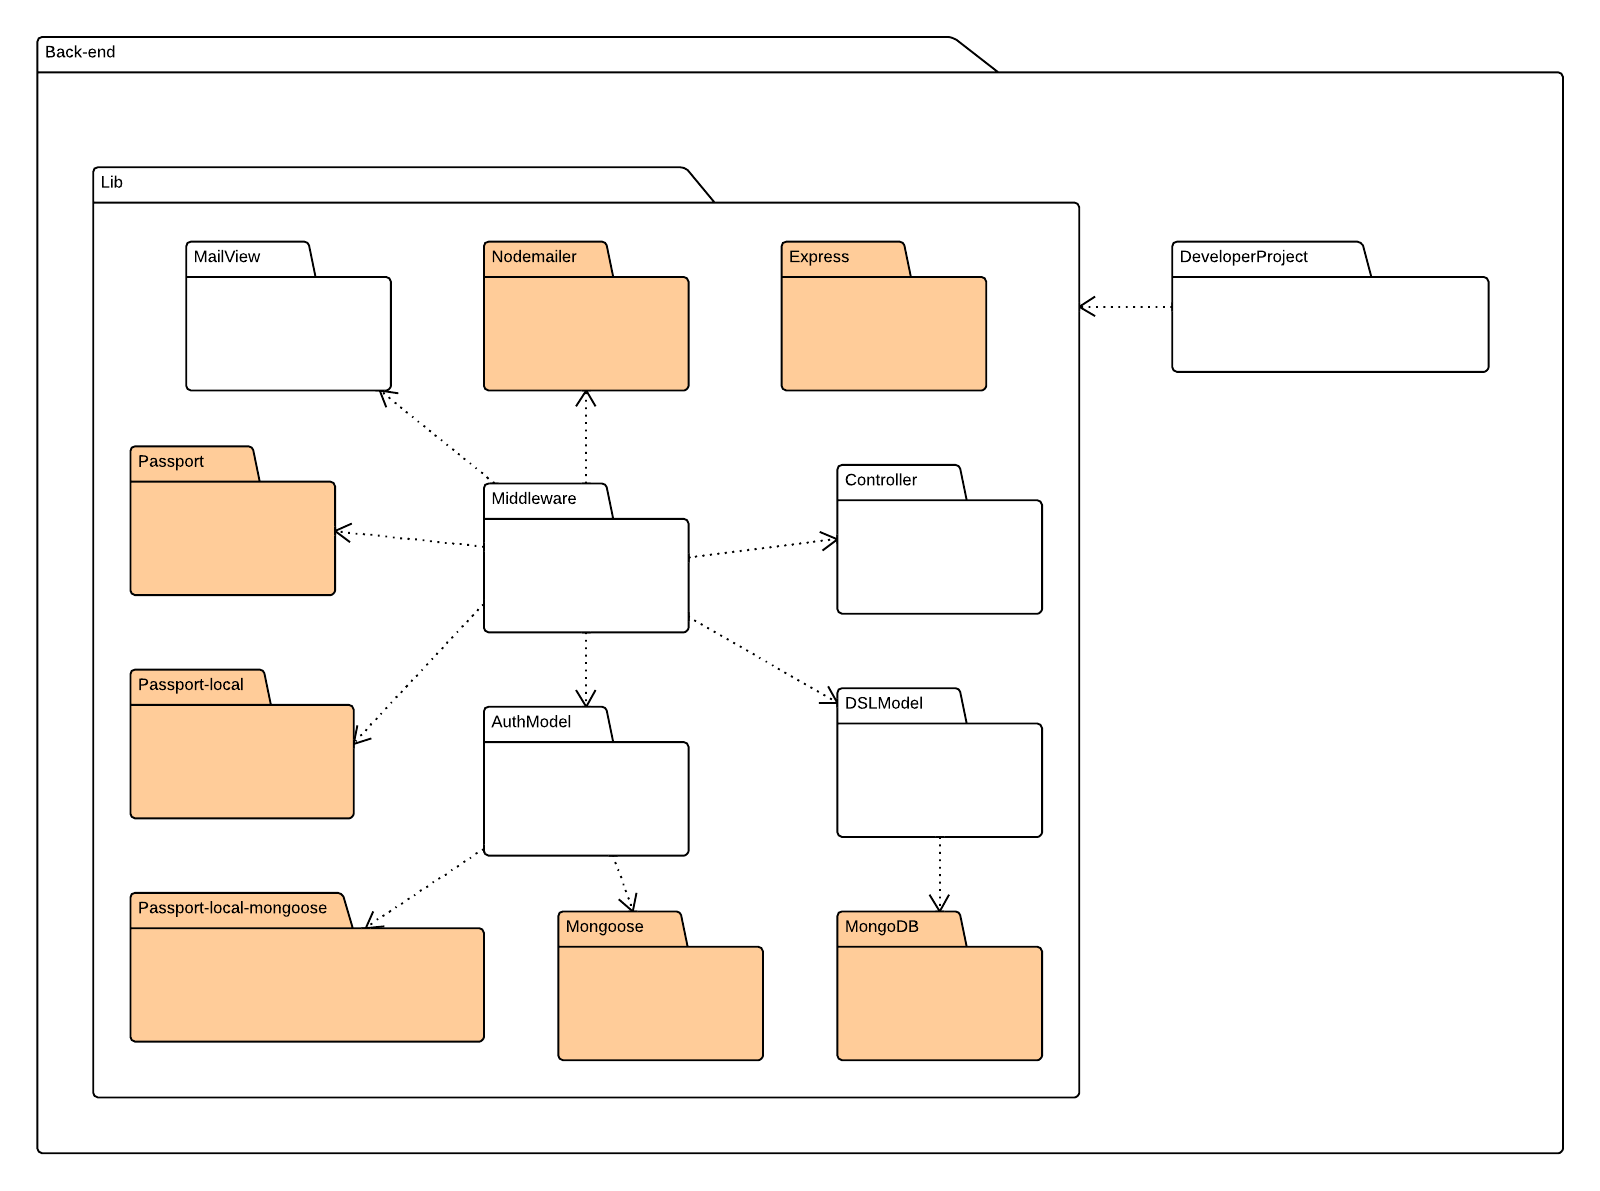
\includegraphics[width=\textwidth]{uml/Back-end-Diagramma dei Packages.png}  
        \caption{Diagramma dei packages Back-end}
      \end{center}  
    \end{figure} 
  \subparagraph{Descrizione} 
    \begin{itemize}
    \item[] \glossario{Package} che racchiude tutta la componente di \glossario{Back-end}. Comprende la libreria dell'applicazione \textit{MaaP} e il package del progetto sviluppato dal developer che andrà ad utilizzare tale libreria. \\ I packages colorati nel diagramma, rappresentano librerie esterne.
    \end{itemize} 
    \subparagraph{Package contenuti} 
    \begin{itemize}
        \item Back-end::DeveloperProject
        \item Back-end::Lib
    \end{itemize}
    
   \subparagraph{Diagramma delle classi}
    \begin{figure}[H] 
      \begin{center} 
        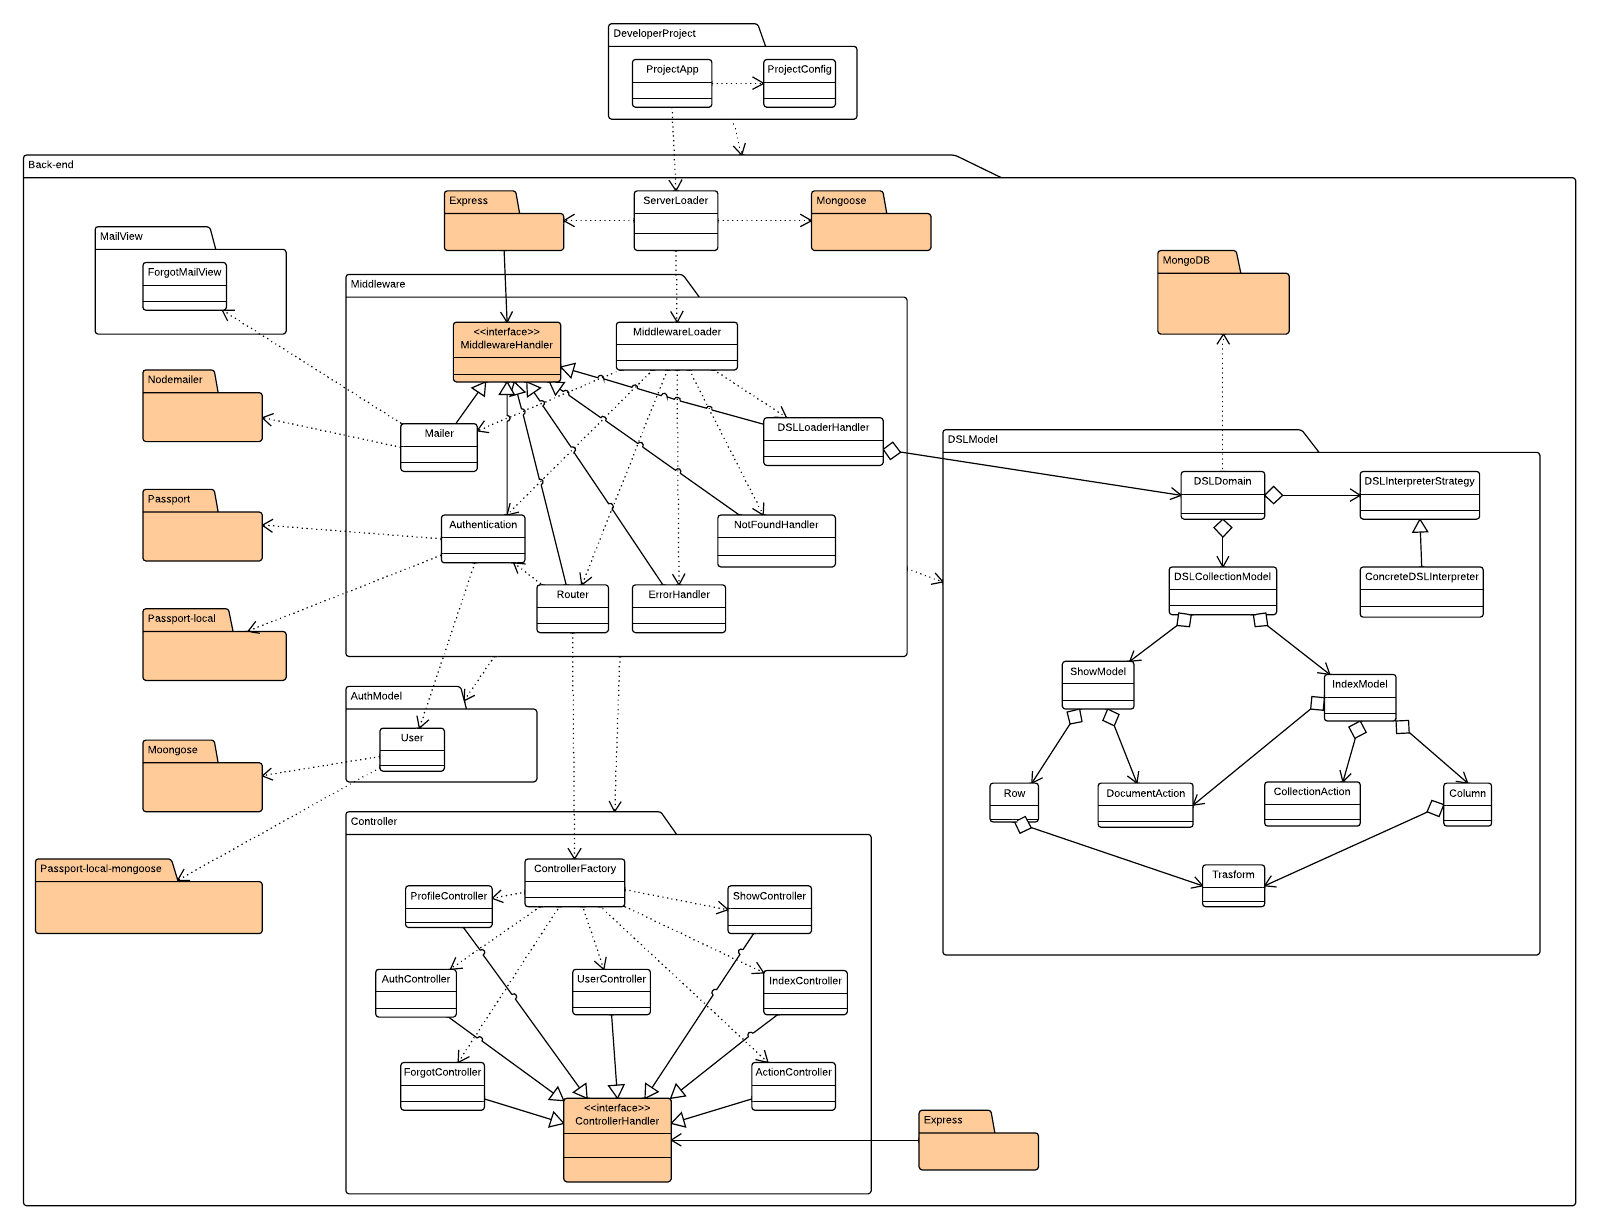
\includegraphics[width=\textwidth]{uml/Back-end-Diagramma delle classi}
        \caption{Diagramma delle classi Back-end}
      \end{center}  
    \end{figure} 
  
  \subsubsection{Back-end::Lib}
  \paragraph{Informazioni sul package} 
    \begin{figure}[H] 
      \begin{center} 
        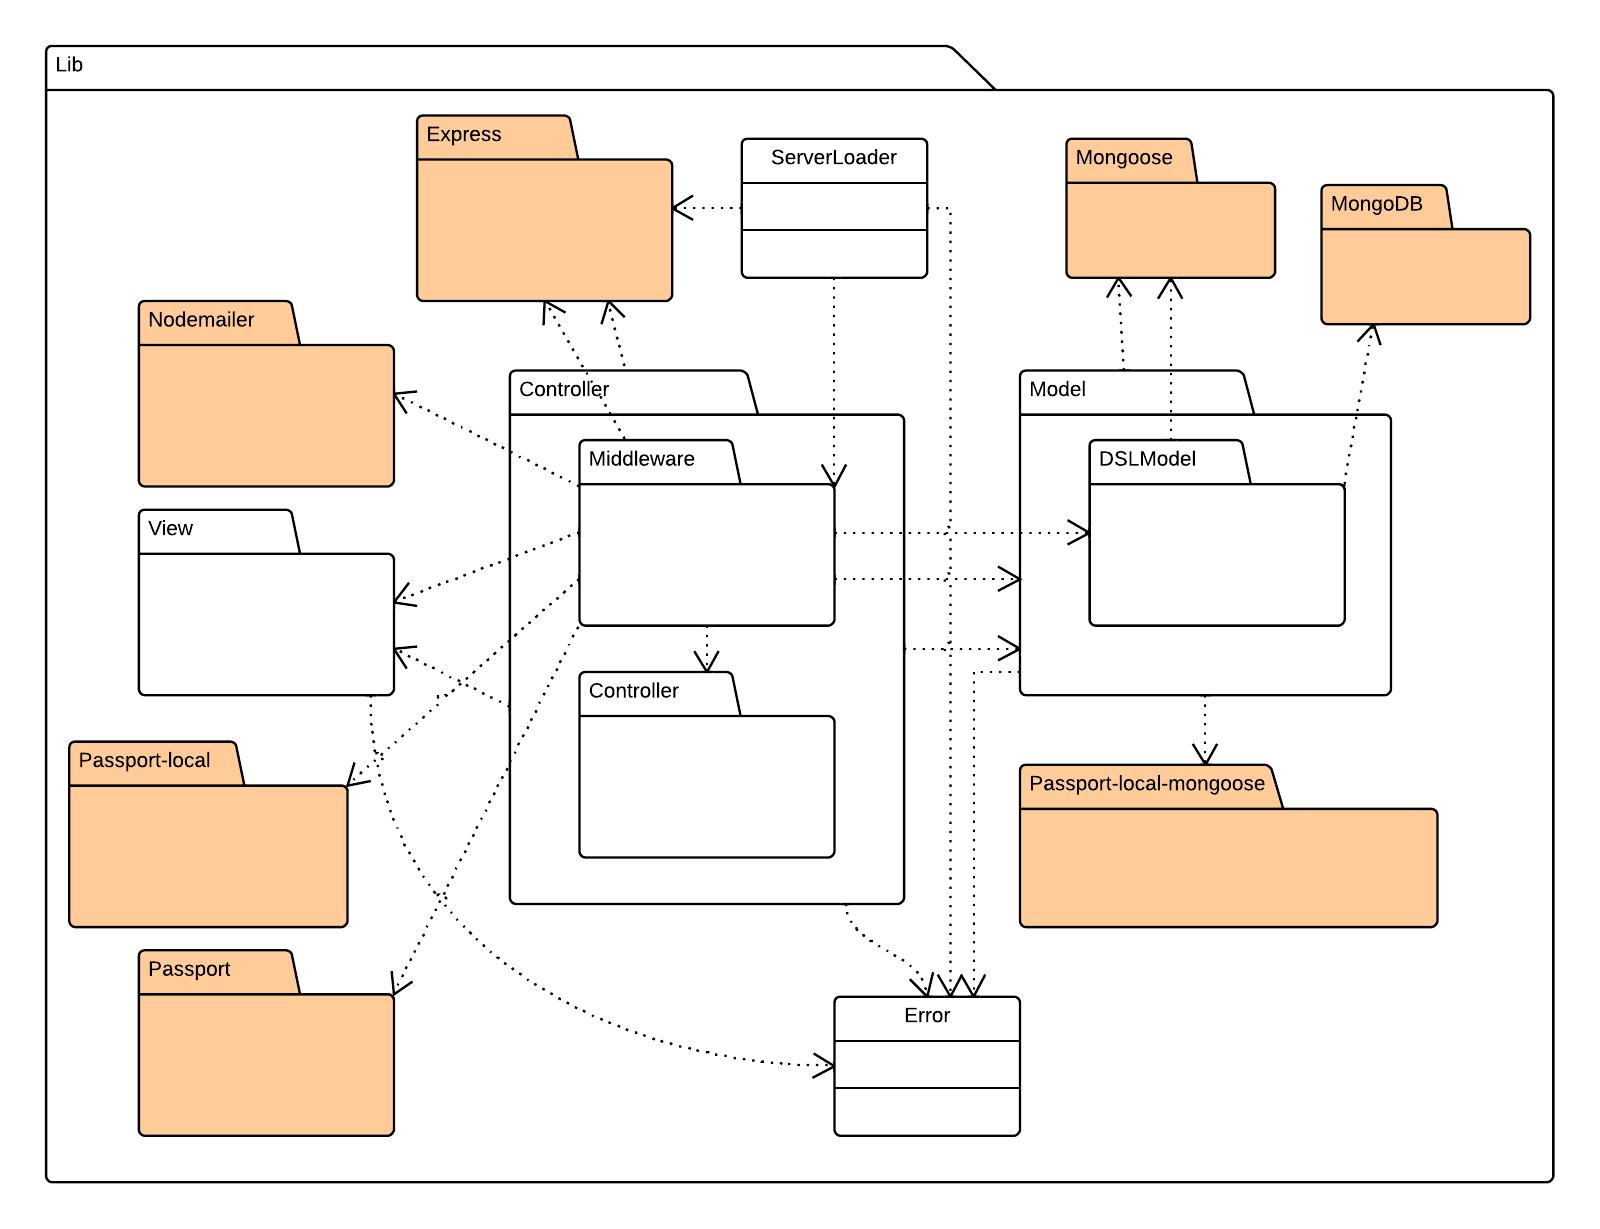
\includegraphics[width=\textwidth]{packages/Back-end::Lib.png}  
        \caption{Componente Back-end::Lib}
      \end{center}  
    \end{figure} 
  \subparagraph{Descrizione} 
    \begin{itemize}
    \item[] \glossario{Package} che costituisce la libreria principale dell'applicazione MaaP, che verrà fornita ai developer per installare e utilizzare l'applicazione. Comprende gli script per l'installazione, non rappresentati nei diagrammi in quanto non sono modellati come oggetti.
    \end{itemize} 
    \subparagraph{Package contenuti} 
    \begin{itemize}
        \item Back-end::Lib::AuthModel
        \item Back-end::Lib::DSLModel
        \item Back-end::Lib::MailView
        \item Back-end::Lib::Middleware
        \item Back-end::Lib::Controller
    \end{itemize}
    
  \subsubsection{Back-end::Lib::AuthModel}
  \paragraph{Informazioni sul package} 
    \begin{figure}[H] 
      \begin{center} 
        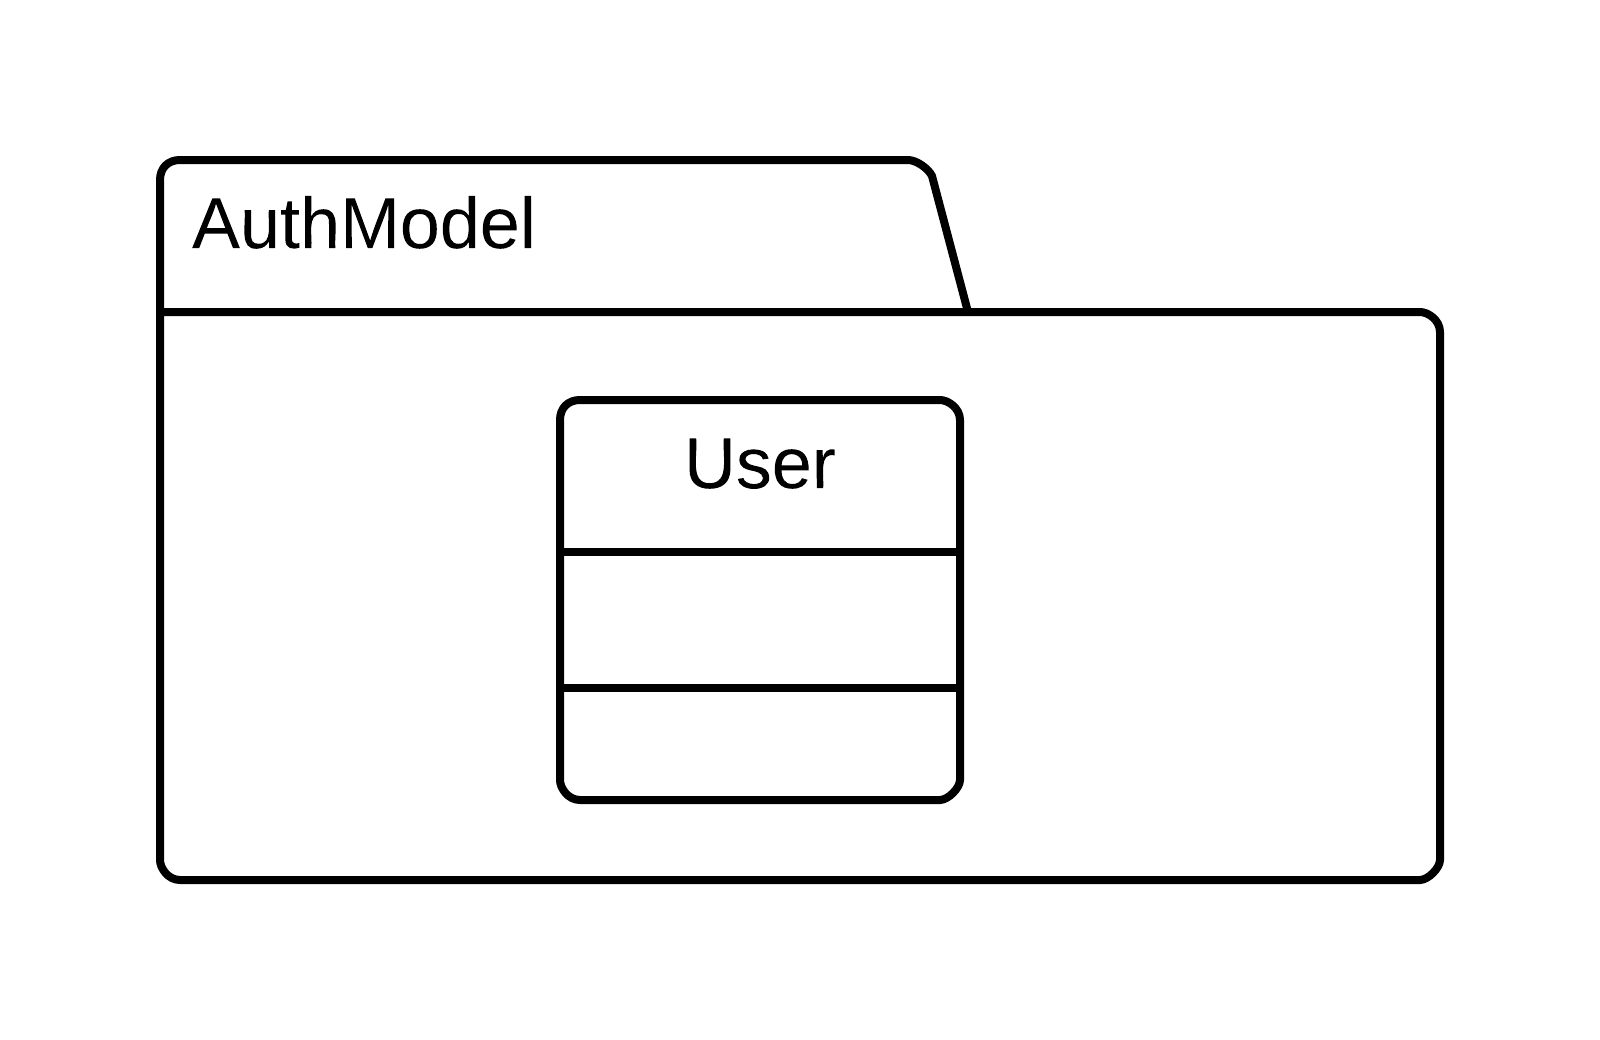
\includegraphics[width=\textwidth]{packages/Back-end::Lib::AuthModel.png}  
        \caption{Componente Back-end::Lib::AuthModel}
      \end{center}  
    \end{figure} 
  \subparagraph{Descrizione} 
    \begin{itemize}
    \item[] \glossario{Package} che gestisce i dati e le operazioni relativi all'autenticazione utente, andando ad aggiungersi alle componenti che compongono la parte model nell'architettura MVC nel back-end. 
    \end{itemize} 
    \paragraph{Classi}
      \subparagraph{Back-end::Lib::AuthModel::User}
        
        \textbf{\\ \\ Descrizione} 
          \begin{itemize}
            \item[] Classe che si occupa dei metodi per la gestione dei dati utente. 
          \end{itemize}      
        \textbf{Utilizzo}  
          \begin{itemize}
            \item[] Viene utilizzata per l'interfacciamento con la libreria \glossario{Mongoose} per la registrazione dello schema dei dati, e con la libreria passport-local-mongoose per il popolamento automatico dello schema con campi dati e metodi predefiniti.
Il costruttore del modello dello schema dei dati viene registrato nella \glossario{Factory} di \glossario{Mongoose} ed ogni istanza condividerà la stessa connessione al server.
          \end{itemize}
  \subsubsection{Back-end::DeveloperProject}
  \paragraph{Informazioni sul package} 
    \begin{figure}[H] 
      \begin{center} 
        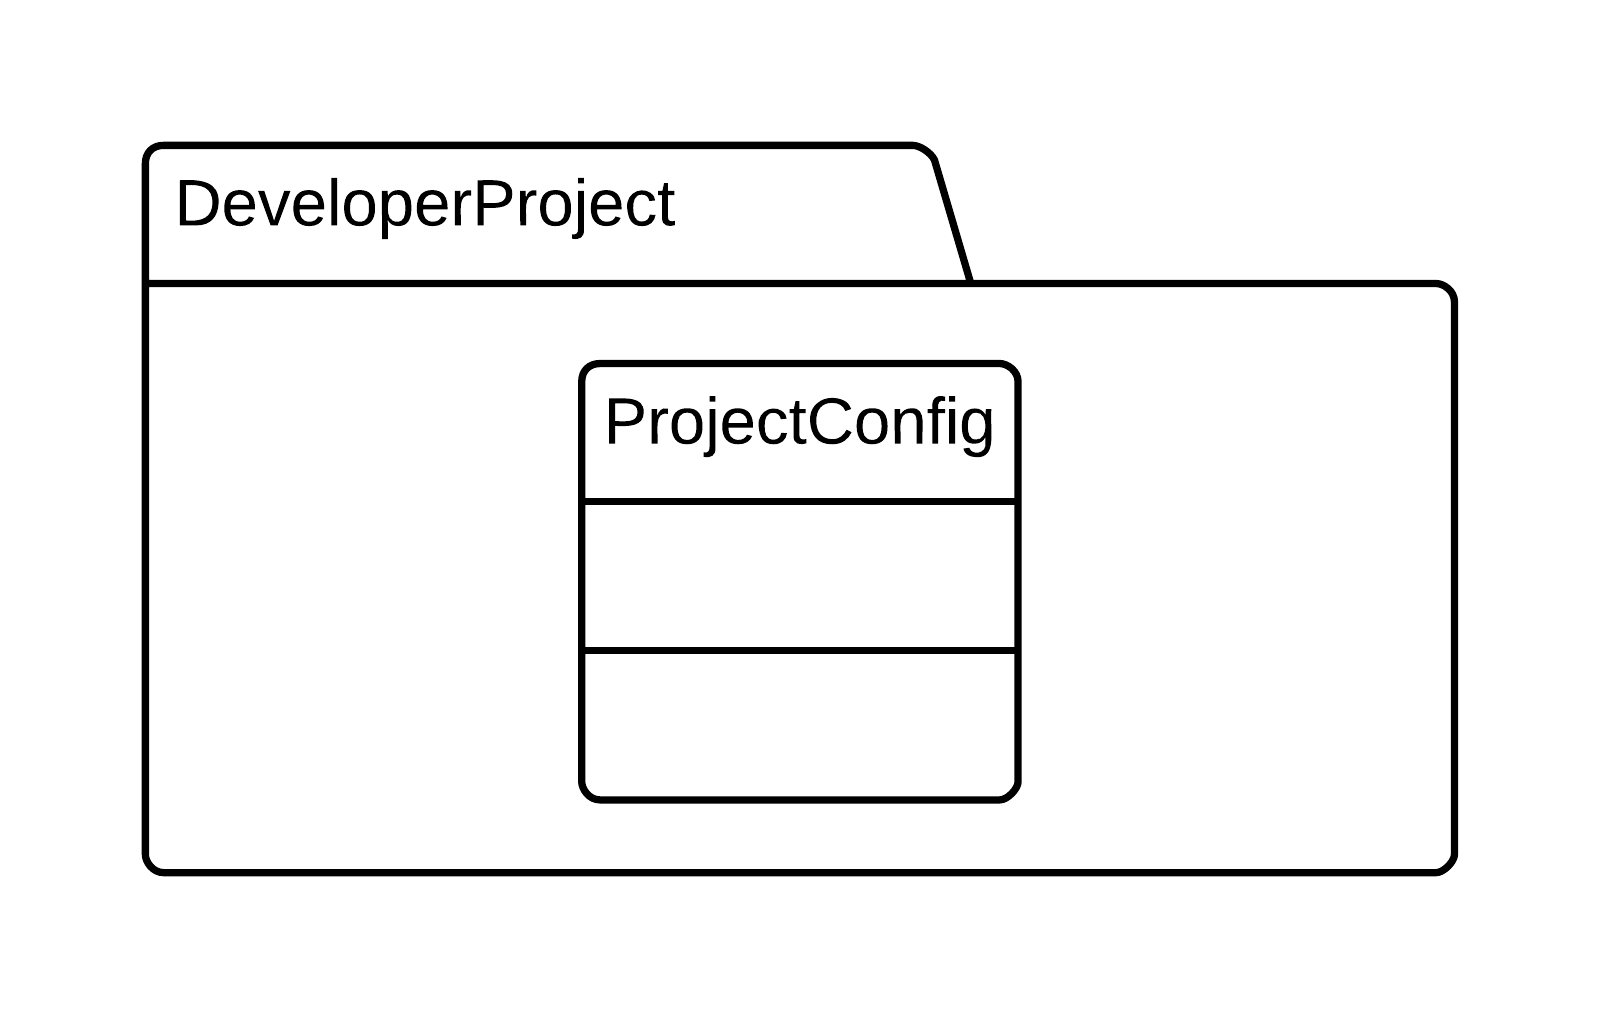
\includegraphics[width=\textwidth]{packages/Back-end::DeveloperProject.png}  
        \caption{Componente Back-end::DeveloperProject}
      \end{center}  
    \end{figure} 
  \subparagraph{Descrizione} 
    \begin{itemize}
    \item[] Questo \glossario{Package} ha il compito di fornire la configurazione e avviare il web server di \glossario{MaaP}. Consiste negli oggetti che dovranno essere predisposti dal developer che vorrà installare il framework \glossario{MaaP}. L'installazione dell framework \glossario{MaaP} fornisce uno \glossario{scaffhold} dei file e delle classi necessarie per il funzionamento dell'applicazione. Sarà compito del developer modificare tali file inserendo i dati corretti.
    \end{itemize} 
    \paragraph{Classi}
      \subparagraph{Back-end::DeveloperProject::ProjectConfig}
        
        \textbf{\\ \\ Descrizione} 
          \begin{itemize}
            \item[] Classe che si occupa di configurare il progetto creato dallo sviluppatore.
          \end{itemize}      
        \textbf{Utilizzo}  
          \begin{itemize}
            \item[] Viene utilizzata per descrivere tutti i parametri dell'applicazione. Quando viene creata una \texttt{Back-end::Lib::ServerApp} le viene passato un oggetto di questo tipo ed essa avvierà l'applicazione a partire da questa configurazione.
          \end{itemize}
  \subsubsection{Back-end::Lib::DSLModel}
  \paragraph{Informazioni sul package} 
    \begin{figure}[H] 
      \begin{center} 
        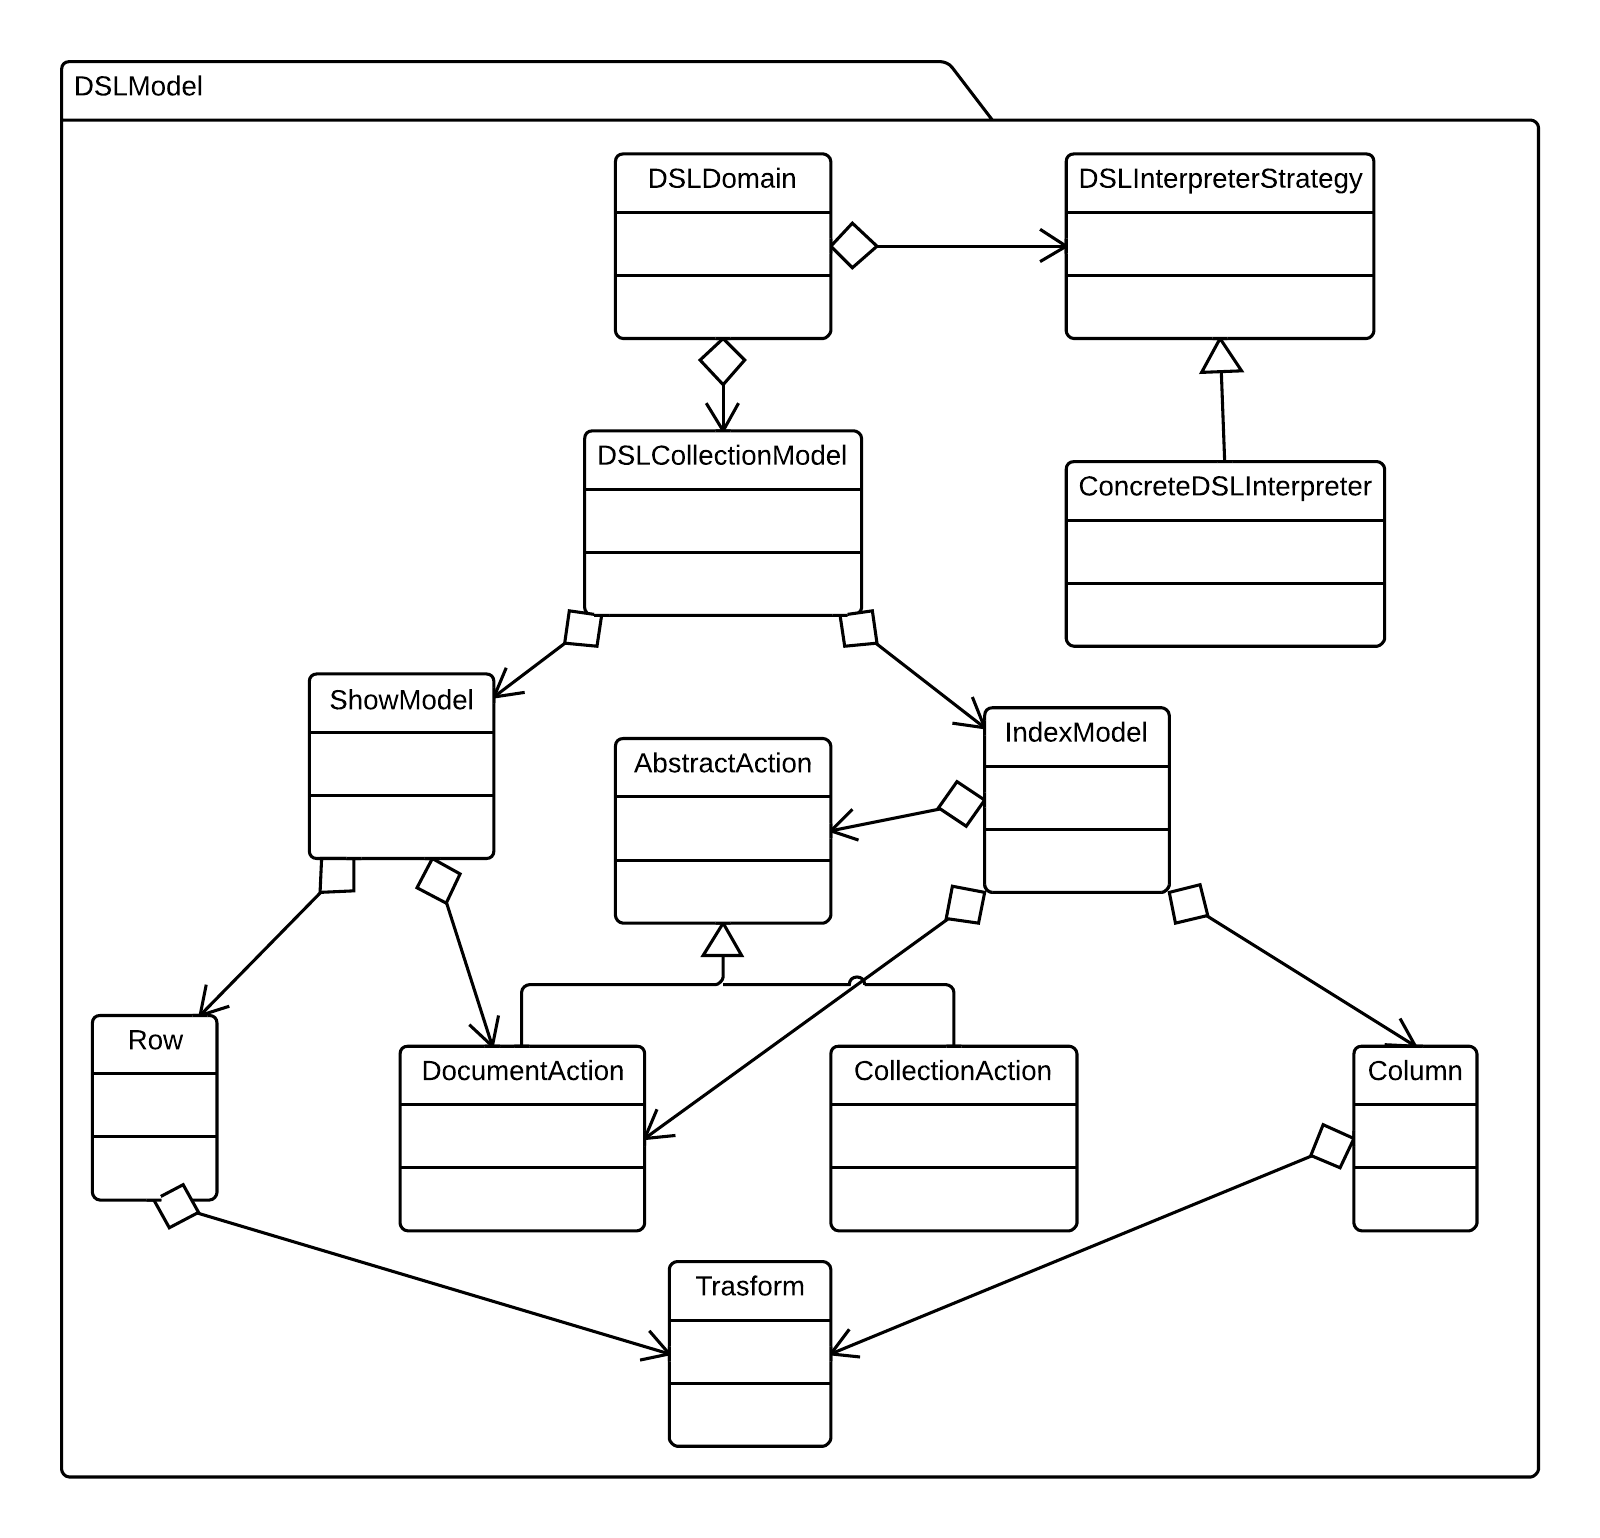
\includegraphics[width=\textwidth]{packages/Back-end::Lib::DSLModel.png}  
        \caption{Componente Back-end::Lib::DSLModel}
      \end{center}  
    \end{figure} 
  \subparagraph{Descrizione} 
    \begin{itemize}
    \item[] \glossario{Package} costituito da classi per la definizione delle regole di business sui dati definite tramite il \glossario{DSL}. 
Il \glossario{package} contiene principalmente classi che si occupano del caricamento del \glossario{DSL} e della sua rappresentazione in un modello ad oggetti. \\
Costituisce la componente model dell'architettura MVC del back-end.
    \end{itemize} 
    \paragraph{Classi}
      \subparagraph{Back-end::Lib::DSLModel::Row}
        
        \textbf{\\ \\ Descrizione} 
          \begin{itemize}
            \item[] Classe che racchiude tutte le informazioni relative ad un elemento (una riga) della show-page. Tali informazioni vengono dichiarate dal developer nel DSL.
          \end{itemize}      
        \textbf{Utilizzo}  
          \begin{itemize}
            \item[] Questa classe viene creata dalla componente che si occupa di caricare il DSL (interpretandolo o facendone il parsing). 
          \end{itemize}
      \subparagraph{Back-end::Lib::DSLModel::AbstractAction}
        
        \textbf{\\ \\ Descrizione} 
          \begin{itemize}
            \item[] Questa classe è una classe astratta che rappresenta le azione definibili dal developer nel DSL, e che potranno essere azionata tramite le \glossario{API} del \glossario{Back-end} per essere eseguite lato-server.
          \end{itemize}      
        \textbf{Utilizzo}  
          \begin{itemize}
            \item[] Questa classe viene utilizzata per raggruppare elementi comuni alle classi DocumentAction e CollectionAction.
          \end{itemize}
          \textbf{Classi Figlie}
          \begin{itemize}
              \item{Back-end::Lib::DSLModel::AbstractAction::CollectionAction}
              \item{Back-end::Lib::DSLModel::AbstractAction::DocumentAction}
          \end{itemize}
      \subparagraph{Back-end::Lib::DSLModel::DSLDomain}
        
        \textbf{\\ \\ Descrizione} 
          \begin{itemize}
            \item[] Classe che si occupa di caricare i file \glossario{DSL}. Implementa il \glossario{Design Pattern} \glossario{registry}.
          \end{itemize}      
        \textbf{Utilizzo}  
          \begin{itemize}
            \item[] Viene utilizzata per caricare dinamicamente tutti i \glossario{DSL} a partire dal \glossario{database} che le viene passato.
          \end{itemize}
          \textbf{Relazioni con altre classi}
          \begin{itemize}
              \item{Back-end::Lib::DSLModel::DSLInterpreterStrategy}
              \item{Back-end::Lib::DSLModel::DSLCollectionModel}
          \end{itemize}
      \subparagraph{Back-end::Lib::DSLModel::DSLInterpreterStrategy}
        
        \textbf{\\ \\ Descrizione} 
          \begin{itemize}
            \item[] Classe astratta che definisce l'interfaccia dell'algoritmo di interpretazione del linguaggio \glossario{DSL} utilizzato. È il componente strategy del \glossario{Design Pattern} \glossario{strategy}.
          \end{itemize}      
        \textbf{Utilizzo}  
          \begin{itemize}
            \item[] Viene utilizzata per incapsulare e rendere intercambiabile l'algoritmo di interpretazione del linguaggio \glossario{DSL}. In questo modo, se in futuro vi fosse necessità di cambiare l'algoritmo di interpretazione l'algoritmo può variare indipendentemente dal client che ne farà uso.
          \end{itemize}
          \textbf{Classi Figlie}
          \begin{itemize}
              \item{Back-end::Lib::DSLModel::DSLInterpreterStrategy::ConcreteDSLInterpreter}
          \end{itemize}
      \subparagraph{Back-end::Lib::DSLModel::DSLCollectionModel}
        
        \textbf{\\ \\ Descrizione} 
          \begin{itemize}
            \item[] Classe che si occupa di definire il model della \glossario{Collection} a partire dal \glossario{DSL}. Si ispira all'\glossario{Abstract Syntax Tree}.
          \end{itemize}      
        \textbf{Utilizzo}  
          \begin{itemize}
            \item[] È l'oggetto risultante dell'interpretazione del \glossario{DSL}. Definisce una rappresentazione interna di una \glossario{Collection}.
          \end{itemize}
          \textbf{Relazioni con altre classi}
          \begin{itemize}
              \item{Back-end::Lib::DSLModel::IndexModel}
              \item{Back-end::Lib::DSLModel::ShowModel}
          \end{itemize}
      \subparagraph{Back-end::Lib::DSLModel::DSLInterpreterStrategy::ConcreteDSLInterpreter}
        
        \textbf{\\ \\ Descrizione} 
          \begin{itemize}
            \item[] Classe che concretizza l'interprete del \glossario{DSL}. È uno dei componenti ConcreteStrategy del \glossario{Design Pattern} \glossario{Strategy}.
          \end{itemize}      
        \textbf{Utilizzo}  
          \begin{itemize}
            \item[] Viene utilizzata per implementare l'algoritmo utilizzato nell'interfaccia \texttt{Back-end::Lib::DSLModel::DSLInterpreterStrategy} per l'interpretazione del linguaggio \glossario{DSL}. Conterrà al suo interno un metodo che genererà il \glossario{parser} a partire da una grammatica regolare.
          \end{itemize}
          \textbf{Classi Ereditate}
          \begin{itemize}
                \item{Back-end::Lib::DSLModel::DSLInterpreterStrategy}
          \end{itemize}
      \subparagraph{Back-end::Lib::DSLModel::IndexModel}
        
        \textbf{\\ \\ Descrizione} 
          \begin{itemize}
            \item[] Classe che racchiude tutte le informazioni relative ad una index-page. Tali informazioni vengono dichiarate dal developer nel DSL. Comprende a sua volta altre classi di tipo Column, DocumentAction e CollectionAction.
          \end{itemize}      
        \textbf{Utilizzo}  
          \begin{itemize}
            \item[] Questa classe viene creata dalla componente che si occupa di caricare il DSL (interpretandolo o facendone il parsing).
          \end{itemize}
          \textbf{Relazioni con altre classi}
          \begin{itemize}
              \item{Back-end::Lib::DSLModel::AbstractAction::CollectionAction}
              \item{Back-end::Lib::DSLModel::AbstractAction::DocumentAction}
          \end{itemize}
      \subparagraph{Back-end::Lib::DSLModel::ShowModel}
        
        \textbf{\\ \\ Descrizione} 
          \begin{itemize}
            \item[] Classe che racchiude tutte le informazioni relative ad una show-page. 
Tali informazioni vengono dichiarate dal developer nel DSL. 
Comprende a sua volta altre classi di tipo Row e DocumentAction.
          \end{itemize}      
        \textbf{Utilizzo}  
          \begin{itemize}
            \item[] Questa classe viene creata dalla componente che si occupa di caricare il DSL (interpretandolo o facendone il parsing).
          \end{itemize}
          \textbf{Relazioni con altre classi}
          \begin{itemize}
              \item{Back-end::Lib::DSLModel::Row}
          \end{itemize}
      \subparagraph{Back-end::Lib::DSLModel::Trasform}
        
        \textbf{\\ \\ Descrizione} 
          \begin{itemize}
            \item[] Classe che racchiude tutte le informazioni relative alla modalità con cui i dati prelevati dal database verranno modificati prima di essere inviati al front-end.
Tali trasformazioni vengono dichiarate dal developer nel DSL.
          \end{itemize}      
        \textbf{Utilizzo}  
          \begin{itemize}
            \item[] Questa classe viene creata dalla componente che si occupa di caricare il DSL (interpretandolo o facendone il parsing).
          \end{itemize}
      \subparagraph{Back-end::Lib::DSLModel::Column}
        
        \textbf{\\ \\ Descrizione} 
          \begin{itemize}
            \item[] Classe che racchiude tutte le informazioni relative ad una riga della show-page. Tali informazioni vengono dichiarate dal developer nel DSL.


          \end{itemize}      
        \textbf{Utilizzo}  
          \begin{itemize}
            \item[] Questa classe viene creata dalla componente che si occupa di caricare il DSL (interpretandolo o facendone il parsing).
          \end{itemize}
          \textbf{Relazioni con altre classi}
          \begin{itemize}
              \item{Back-end::Lib::DSLModel::Trasform}
          \end{itemize}
      \subparagraph{Back-end::Lib::DSLModel::AbstractAction::CollectionAction}
        
        \textbf{\\ \\ Descrizione} 
          \begin{itemize}
            \item[] Questa classe descrive un azione definita dal developer nel DSL, che potrà essere azionata tramite le \glossario{API} del \glossario{Back-end} ed eseguita lato-server. Tale azione potrà eseguire operazioni sulla collection corrispondente al DSLCollectionModel che contiene indirettamente questa classe. La classe assume il ruolo di Command descritto dal \glossario{design pattern} Command. Gli oggetti che avranno il ruolo di ConcreteCommand verranno creati dinamicamente, definendo a run-time dei metodi aggiuntivi per questa classe.
          \end{itemize}      
        \textbf{Utilizzo}  
          \begin{itemize}
            \item[] Questa classe viene creata dalla componente che si occupa di caricare il DSL (interpretandolo o facendone il parsing).
          \end{itemize}
          \textbf{Classi Ereditate}
          \begin{itemize}
                \item{Back-end::Lib::DSLModel::AbstractAction}
          \end{itemize}
      \subparagraph{Back-end::Lib::DSLModel::AbstractAction::DocumentAction}
        
        \textbf{\\ \\ Descrizione} 
          \begin{itemize}
            \item[] Questa classe descrive un azione definita dal developer nel DSL, che potrà essere azionata tramite le \glossario{API} del \glossario{Back-end} ed eseguita lato-server. Tale azione potrà eseguire operazioni su un document della collection corrispondente al DSLCollectionModel che contiene indirettamente questa classe. La classe assume il ruolo di Command descritto dal \glossario{design pattern} Command. Gli oggetti che avranno il ruolo di ConcreteCommand verranno creati dinamicamente, definendo a run-time dei metodi aggiuntivi per questa classe.
          \end{itemize}      
        \textbf{Utilizzo}  
          \begin{itemize}
            \item[] Questa classe viene creata dalla componente che si occupa di caricare il DSL (interpretandolo o facendone il parsing). 
          \end{itemize}
          \textbf{Classi Ereditate}
          \begin{itemize}
                \item{Back-end::Lib::DSLModel::AbstractAction}
          \end{itemize}
  
  \subsubsection{Back-end::Lib::MailView}
  \paragraph{Informazioni sul package} 
    \begin{figure}[H] 
      \begin{center} 
        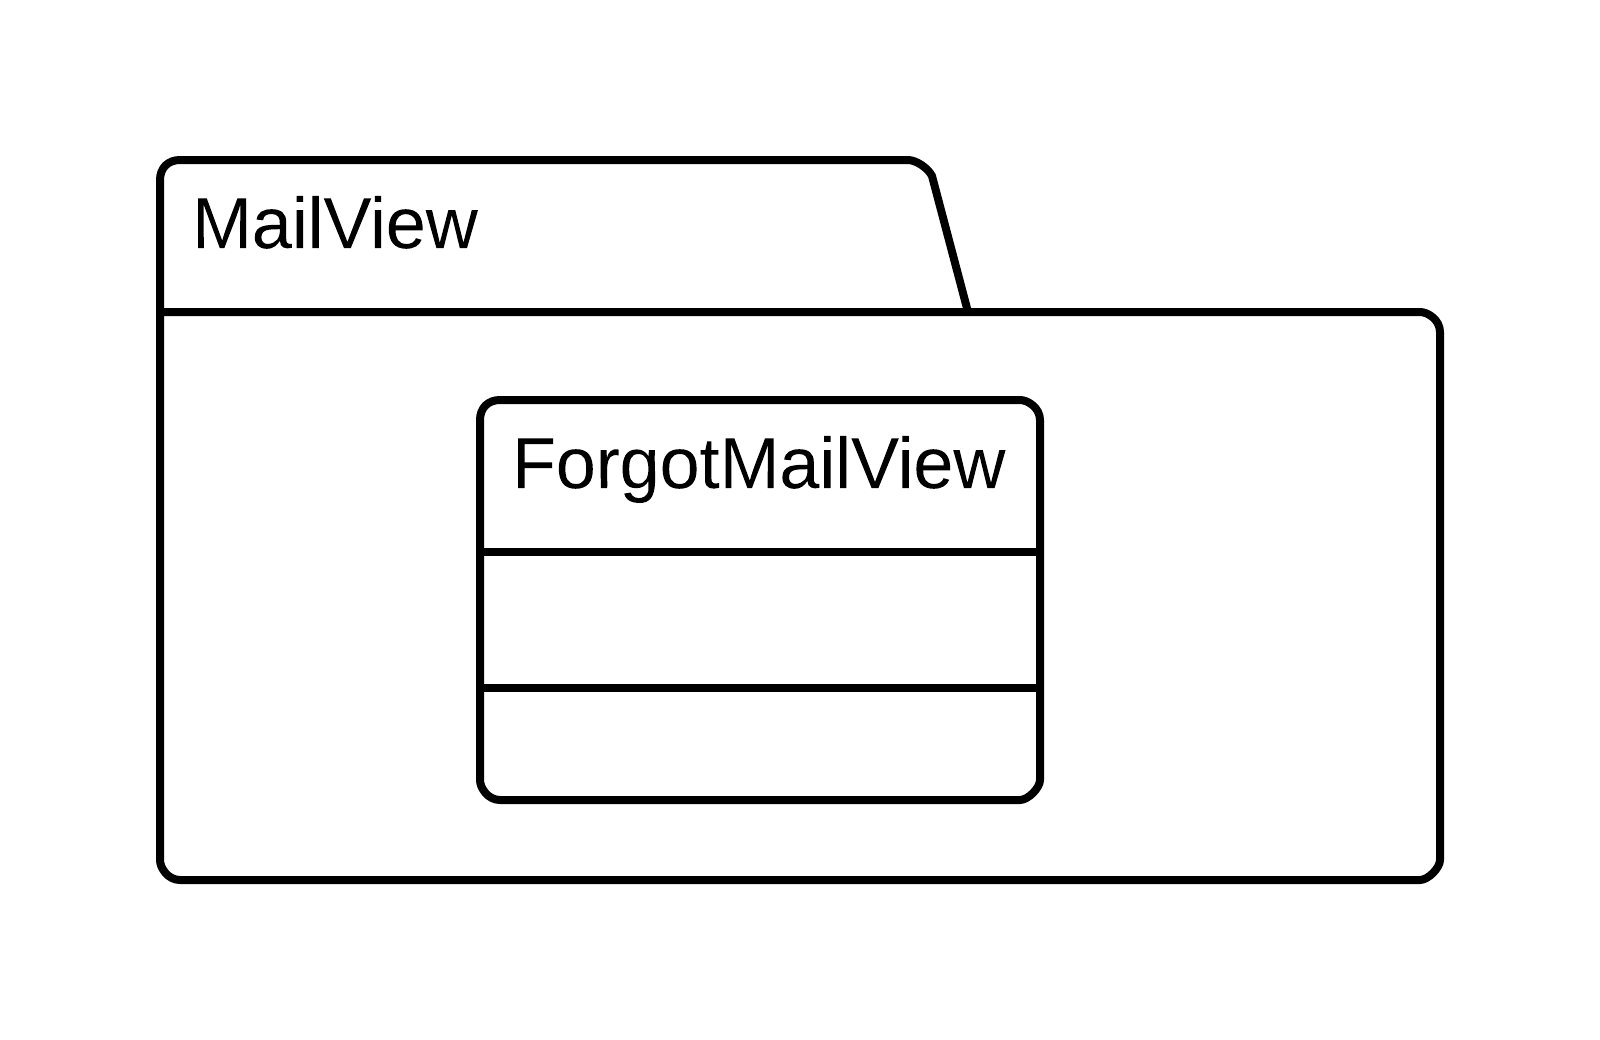
\includegraphics[width=\textwidth]{packages/Back-end::Lib::MailView.png}  
        \caption{Componente Back-end::Lib::MailView}
      \end{center}  
    \end{figure} 
  \subparagraph{Descrizione} 
    \begin{itemize}
    \item[] \glossario{Package} contenente le classi che costituiscono i template utilizzati per le email di recupero-password. Verranno utilizzate dal \glossario{middleware} Mailer.
    \end{itemize} 
    \paragraph{Classi}
      \subparagraph{Back-end::Lib::MailView::ForgotMailView}
        
        \textbf{\\ \\ Descrizione} 
          \begin{itemize}
            \item[] Classe che fornisce una rappresentazione della mail.
          \end{itemize}      
        \textbf{Utilizzo}  
          \begin{itemize}
            \item[] Viene utilizzata come template di email da inviare nel caso in cui l'utente richieda il recupero password.
          \end{itemize}
  \subsubsection{Back-end::Lib::Middleware}
  \paragraph{Informazioni sul package} 
    \begin{figure}[H] 
      \begin{center} 
        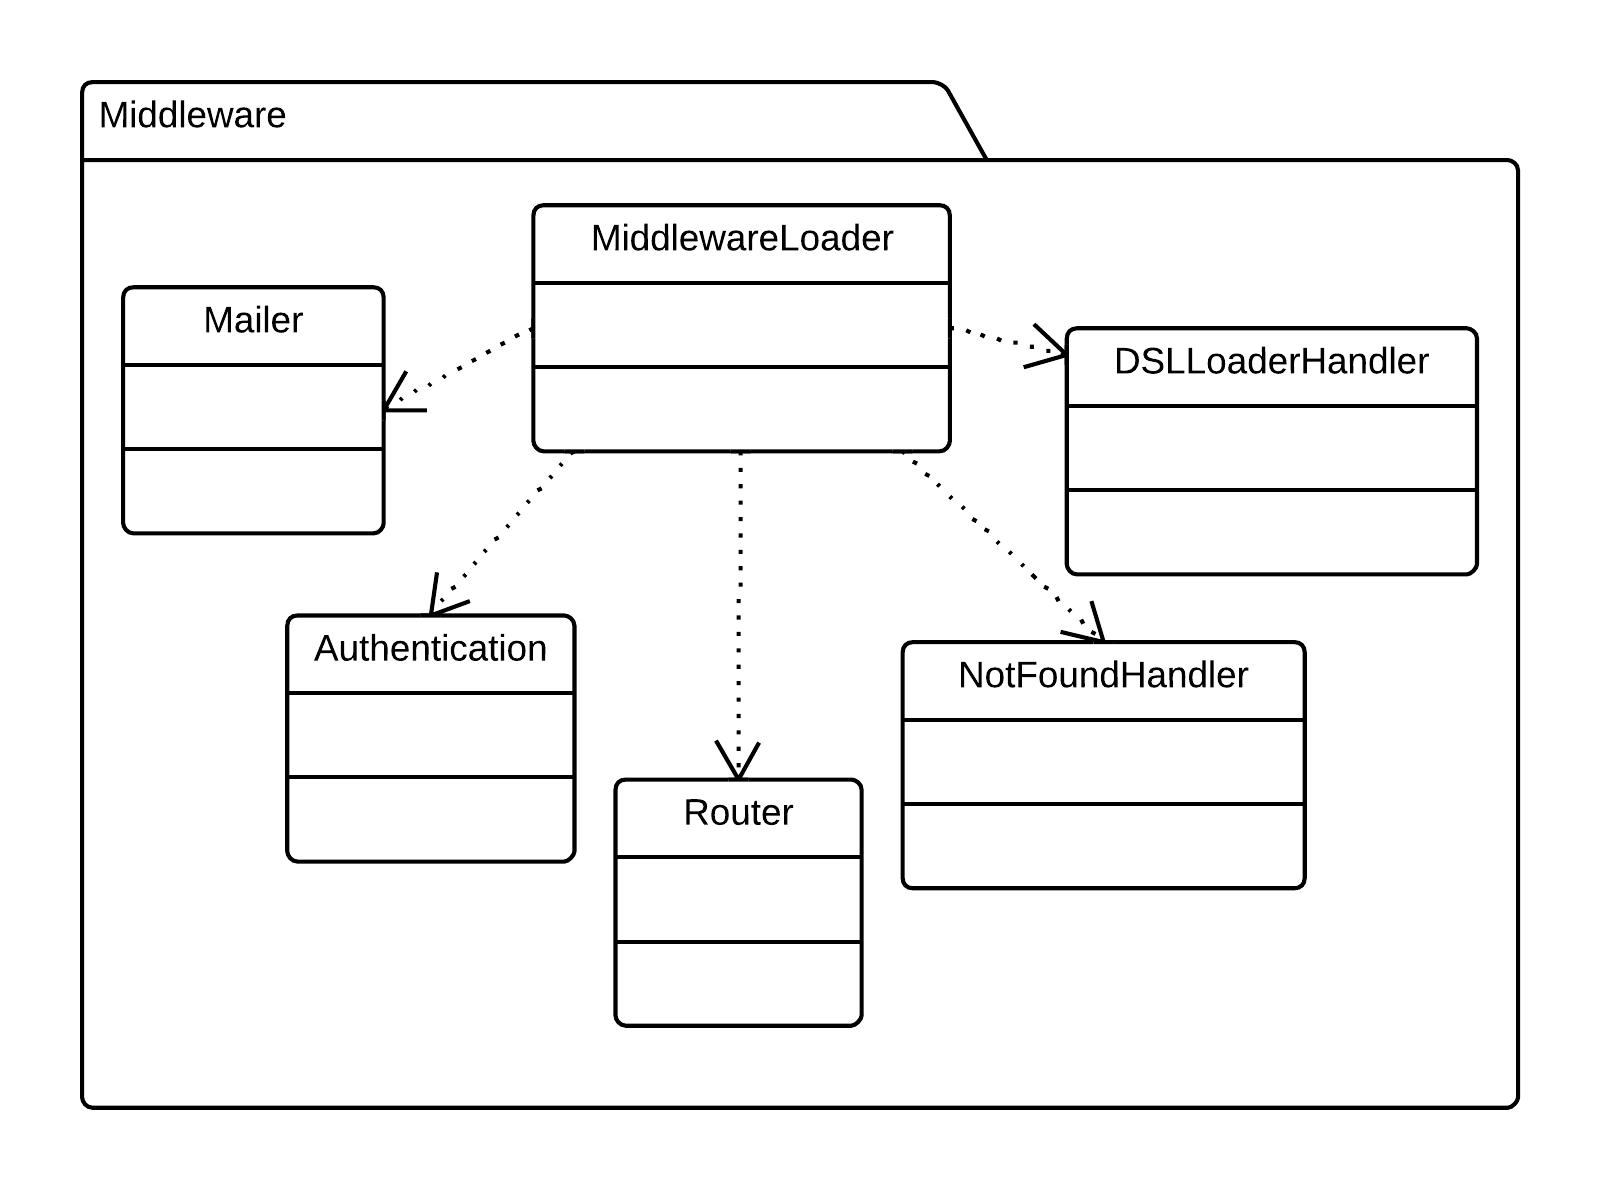
\includegraphics[width=\textwidth]{packages/Back-end::Lib::Middleware.png}  
        \caption{Componente Back-end::Lib::Middleware}
      \end{center}  
    \end{figure} 
  \subparagraph{Descrizione} 
    \begin{itemize}
    \item[] \glossario{Package} contenente classi che costituiscono gli handler della catena di chiamate a cui viene passata la responsabilità di gestire una richiesta,  decorando quest'ultima con parametri e metodi utilizzabili dai controller. Costituisce una parte dell' \glossario{application logic} nell'architettura \glossario{MVC} del \glossario{Back-end}.
    \end{itemize} 
    \paragraph{Classi}
      \subparagraph{Back-end::Lib::Middleware::Router}
        
        \textbf{\\ \\ Descrizione} 
          \begin{itemize}
            \item[] Classe che si occupa della richiesta di risorse. È uno dei componenti subsystem class del \glossario{Design Pattern} \glossario{Facade} e handler del \glossario{Design Pattern} \glossario{Chain of responsability}.
          \end{itemize}      
        \textbf{Utilizzo}  
          \begin{itemize}
            \item[] Si occupa di smistare la richiesta in base all'\glossario{URI} ricevuto e ad invocare l'opportuno metodo di creazione sulla classe \texttt{Back-end::Lib::Controller::ControllerFactory}.
          \end{itemize}
      \subparagraph{Back-end::Lib::Middleware::Authentication}
        
        \textbf{\\ \\ Descrizione} 
          \begin{itemize}
            \item[] Classe che si occupa dell'autenticazione di un'utente. È uno dei componenti subsystem class del \glossario{Design Pattern} \glossario{Facade} e handler del \glossario{Design Pattern} \glossario{Chain of responsability}.
          \end{itemize}      
        \textbf{Utilizzo}  
          \begin{itemize}
            \item[] Viene utilizzata per verificare i dati inseriti dall'utente nella pagina di login e controllare l'effettiva corrispondenza delle credenziali nel \glossario{database}.
          \end{itemize}
          \textbf{Relazioni con altre classi}
          \begin{itemize}
              \item{Back-end::Lib::AuthModel::User}
          \end{itemize}
      \subparagraph{Back-end::Lib::Middleware::DSLLoaderHandler}
        
        \textbf{\\ \\ Descrizione} 
          \begin{itemize}
            \item[] Classe che si occupa di caricare i \glossario{DSL} presenti nel sistema. È uno dei componenti subsystem class del \glossario{Design Pattern} \glossario{Facade} e handler del \glossario{Design Pattern} \glossario{Chain of responsability}.
          \end{itemize}      
        \textbf{Utilizzo}  
          \begin{itemize}
            \item[] Viene utilizzata per caricare i \glossario{DSL} delle \glossario{Collection} all'interno del \glossario{database}.
          \end{itemize}
          \textbf{Relazioni con altre classi}
          \begin{itemize}
              \item{Back-end::Lib::DSLModel::DSLDomain}
          \end{itemize}
      \subparagraph{Back-end::Lib::Middleware::Mailer}
        
        \textbf{\\ \\ Descrizione} 
          \begin{itemize}
            \item[] Classe che si occupa dell'invio di email. È uno dei componenti subsystem class del \glossario{Design Pattern} \glossario{Facade} e handler del \glossario{Design Pattern} \glossario{Chain of responsability}.
          \end{itemize}      
        \textbf{Utilizzo}  
          \begin{itemize}
            \item[] Viene utilizzata per inviare un'email ad un utente che ha effettuato la richiesta di recupero password.
          \end{itemize}
          \textbf{Relazioni con altre classi}
          \begin{itemize}
              \item{Back-end::Lib::MailView::ForgotMailView}
          \end{itemize}
      \subparagraph{Back-end::Lib::Middleware::MiddlewareLoader}
        
        \textbf{\\ \\ Descrizione} 
          \begin{itemize}
            \item[] Classe che definisce un'interfaccia comune per tutte le richieste dell'applicazione. È la componente facade del \glossario{Design Pattern} \glossario{Facade} e handler del \glossario{Design Pattern} \glossario{Chain of responsability}.
          \end{itemize}      
        \textbf{Utilizzo}  
          \begin{itemize}
            \item[] Viene utilizzato per istanziare in modo "nascosto" all'applicazione tutti i \glossario{middleware} presenti nel componente \texttt{Back-end::Lib::Middleware}.
          \end{itemize}
          \textbf{Relazioni con altre classi}
          \begin{itemize}
              \item{Back-end::Lib::Middleware::Router}
              \item{Back-end::Lib::Middleware::Authentication}
              \item{Back-end::Lib::Middleware::DSLLoaderHandler}
              \item{Back-end::Lib::Middleware::Mailer}
              \item{Back-end::Lib::Middleware::NotFoundHandler}
          \end{itemize}
      \subparagraph{Back-end::Lib::Middleware::NotFoundHandler}
        
        \textbf{\\ \\ Descrizione} 
          \begin{itemize}
            \item[] Classe che si occupa la gestione dell'errore di pagina non trovata. È uno dei componenti subsystem class del \glossario{Design Pattern} \glossario{Facade} e handler del \glossario{Design Pattern} \glossario{Chain of responsability}.
          \end{itemize}      
        \textbf{Utilizzo}  
          \begin{itemize}
            \item[] Viene utilizzata per generare una pagina 404 di errore nel caso in cui l'\glossario{URI} passato non corrisponda ad una risorsa presente nell'applicazione.
          \end{itemize}
      \subparagraph{Back-end::Lib::Middleware::Errorhandler}
        
        \textbf{\\ \\ Descrizione} 
          \begin{itemize}
            \item[] Questa classe gestisce gli errori generati nei precedenti middleware o controller. Invia al client una risposta con stato HTTP 500 (server error) con una descrizione dell'errore nel formato JSON.
È uno dei componenti subsystem class del \glossario{Design Pattern} \glossario{Facade} e handler del \glossario{Design Pattern} \glossario{Chain of responsability}.
          \end{itemize}      
        \textbf{Utilizzo}  
          \begin{itemize}
            \item[] Questo middleware viene utilizzato per ultimo nella catena di gestione delle richieste di Express, in modo da gestire tutti gli errori generati precedentemente.
          \end{itemize}
  \subsubsection{Back-end::Lib::Controller}
  \paragraph{Informazioni sul package} 
    \begin{figure}[H] 
      \begin{center} 
        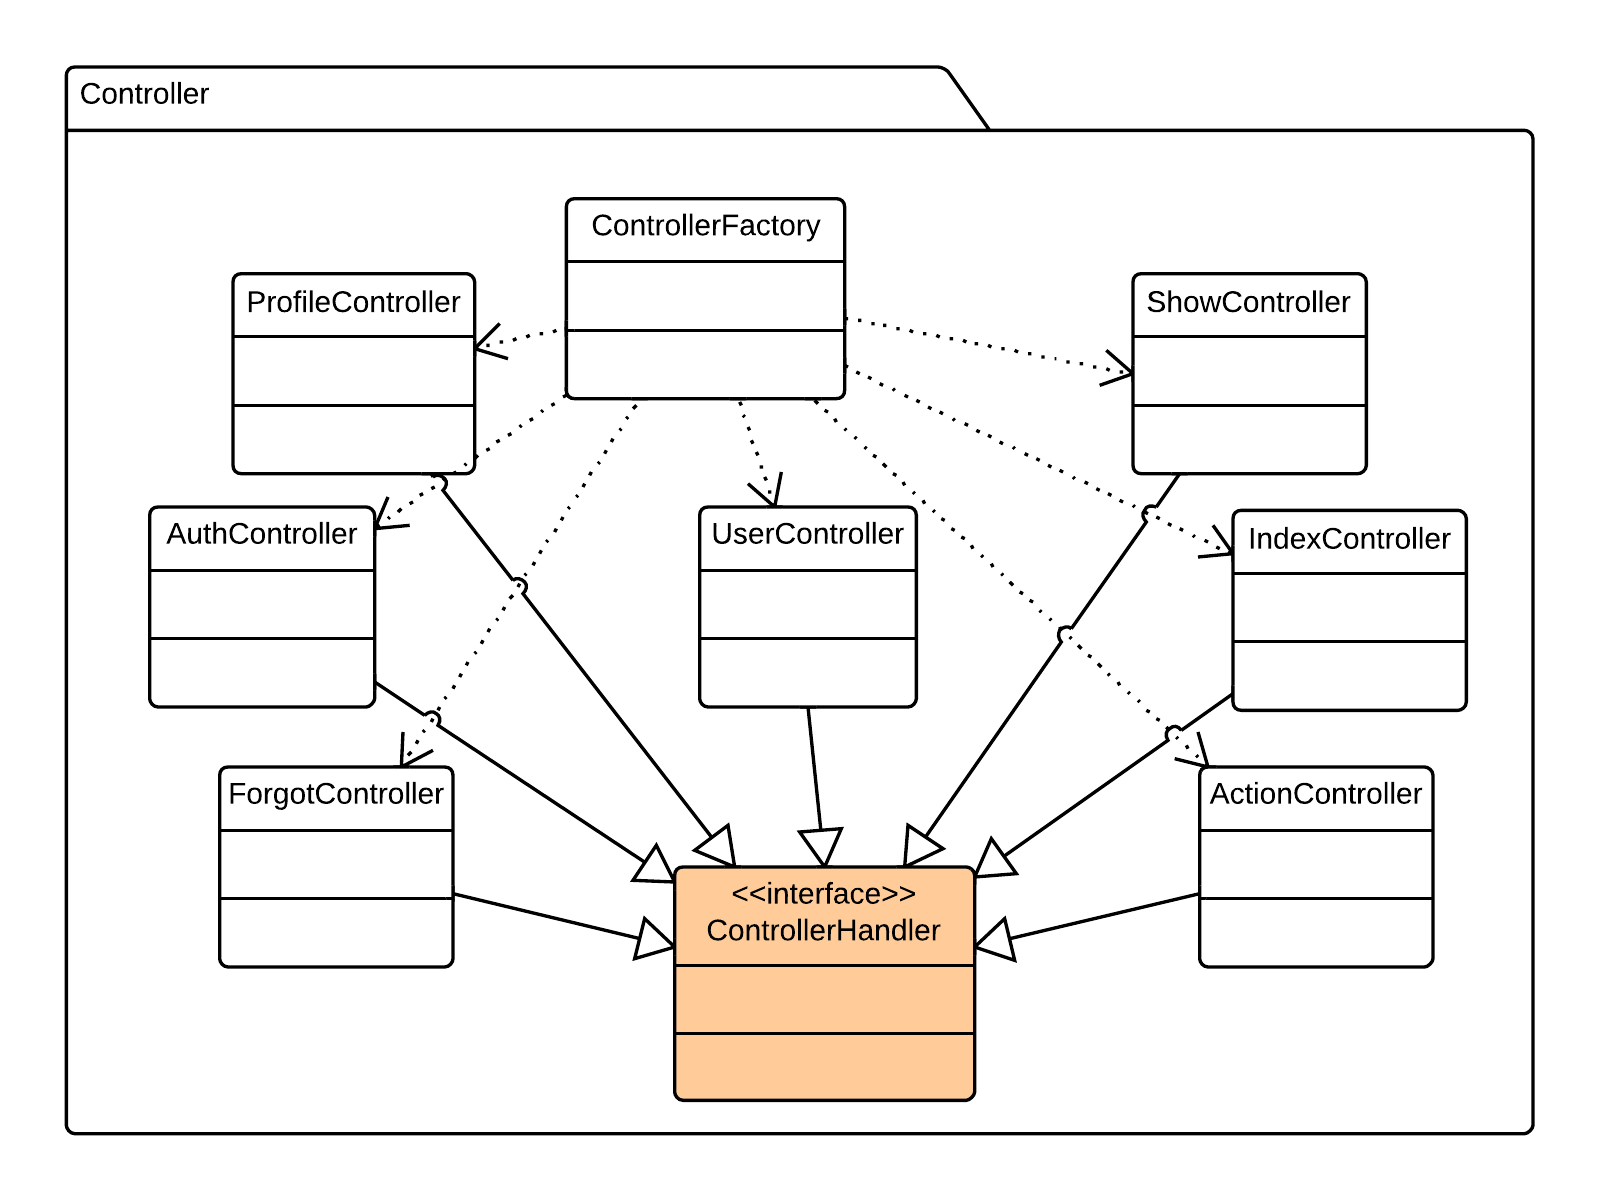
\includegraphics[width=\textwidth]{packages/Back-end::Lib::Controller.png}  
        \caption{Componente Back-end::Lib::Controller}
      \end{center}  
    \end{figure} 
  \subparagraph{Descrizione} 
    \begin{itemize}
    \item[] \glossario{Package} per il componente che realizza parte controller nell'architettura mvc nel back-end. Contiene classi per le funzionalità di controllo e visualizzazione delle risorse, dove ogni classe gestisce in modo esclusivo una sola di queste, in base all' \glossario{URI}.
    \end{itemize} 
    \paragraph{Classi}
      \subparagraph{Back-end::Lib::Controller::UserController}
        
        \textbf{\\ \\ Descrizione} 
          \begin{itemize}
            \item[] Classe che si occupa della varie operazioni che l'admin può compiere sugli utenti dell'applicazione. È uno dei componenti product del \glossario{Design Pattern} \glossario{Factory method}.
          \end{itemize}      
        \textbf{Utilizzo}  
          \begin{itemize}
            \item[] Viene utilizzata per visualizzare la \glossario{index-page} degli utenti, visualizzare le relative \glossario{show-page}, eliminare un utente e modificare il profilo. Mette a disposizione dei metodi per effettuare tutte queste operazioni.
          \end{itemize}
      \subparagraph{Back-end::Lib::Controller::ActionController}
        
        \textbf{\\ \\ Descrizione} 
          \begin{itemize}
            \item[] Classe che rappresenta i metodi per la gestione della risorsa corrispondente ad un'azione. 
È uno dei componenti product del \glossario{Design Pattern} \glossario{Factory method}.
          \end{itemize}      
        \textbf{Utilizzo}  
          \begin{itemize}
            \item[] Viene utilizzata per gestire le azioni personalizzate predisposte nelle pagine index-page e show-page, delegando alla classe \texttt{Back-end::Lib::DSLModel::DSLDomain} la loro esecuzione avendo quest'ultima l'implementazione delle stesse. 
          \end{itemize}
      \subparagraph{Back-end::Lib::Controller::ControllerFactory}
        
        \textbf{\\ \\ Descrizione} 
          \begin{itemize}
            \item[] Classe che si occupa di istanziare e restituire una classe \textit{Controller}. Rappresenta il componente creator del \glossario{Design Pattern} \glossario{Factory method}.
          \end{itemize}      
        \textbf{Utilizzo}  
          \begin{itemize}
            \item[] Viene costruita una sola volta dalla classe \texttt{Back-end::Lib::Middleware::Router} e si occupa di creare e restituire l'oggetto \textit{Controller} richiesto.
          \end{itemize}
      \subparagraph{Back-end::Lib::Controller::AuthController}
        
        \textbf{\\ \\ Descrizione} 
          \begin{itemize}
            \item[] Classe che rappresenta i metodi per la gestione delle risorse di login e logout. È uno dei componenti product del \glossario{Design Pattern} \glossario{Factory method}.

          \end{itemize}      
        \textbf{Utilizzo}  
          \begin{itemize}
            \item[] Viene utilizzata per gestire i dati di e le operazioni relativi all'autenticazione utente e al suo logout dall'applicazione, occupandosi della creazione della sessione utente e della sua distruzione tramite \glossario{cookies}.
          \end{itemize}
      \subparagraph{Back-end::Lib::Controller::ProfileController}
        
        \textbf{\\ \\ Descrizione} 
          \begin{itemize}
            \item[] Classe che rappresenta la gestione di un profilo utente. È uno dei componenti product del \glossario{Design Pattern} \glossario{Factory method}.
          \end{itemize}      
        \textbf{Utilizzo}  
          \begin{itemize}
            \item[] Viene utilizzata per visualizzare il profilo dell'utente, tramite GET, e per editarlo tramite PUT.
          \end{itemize}
      \subparagraph{Back-end::Lib::Controller::ShowController}
        
        \textbf{\\ \\ Descrizione} 
          \begin{itemize}
            \item[] Classe che si occupa della gestione della risorsa show-page.
È uno dei componenti product del \glossario{Design Pattern} \glossario{Factory method}.
          \end{itemize}      
        \textbf{Utilizzo}  
          \begin{itemize}
            \item[] Viene utilizzata per gestire una richiesta della risorsa show-page, delegando alla classe \texttt{Back-end::Lib::DSLModel::DSLDomain} la sua visualizzazione.
          \end{itemize}
      \subparagraph{Back-end::Lib::Controller::IndexController}
        
        \textbf{\\ \\ Descrizione} 
          \begin{itemize}
            \item[] Classe di gestione per la risorsa index 
È uno dei componenti product del \glossario{Design Pattern} \glossario{Factory method}.

          \end{itemize}      
        \textbf{Utilizzo}  
          \begin{itemize}
            \item[] Viene utilizzata per gestire la risorsa corrispondente all'index-page di un \glossario{Document}, offrendo metodi per restituirne gli attributi, effettuarne la modifica o la cancellazione e delega la visualizzazione dell'index-page alla classe \texttt{Back-end::Lib::DSLModel::DSLDomain}.

          \end{itemize}
      \subparagraph{Back-end::Lib::Controller::ForgotController}
        
        \textbf{\\ \\ Descrizione} 
          \begin{itemize}
            \item[] Classe che rappresenta il sistema di recupero e ripristino password. È uno dei componenti product del \glossario{Design Pattern} \glossario{Factory method}.
          \end{itemize}      
        \textbf{Utilizzo}  
          \begin{itemize}
            \item[] La classe fornisce dei metodi per effettuare una richiesta di reset password e, in un secondo momento, procedere al suo ripristino. La richiesta di reset avviene mandando un'email all'indirizzo dell'utente tramite la classe \texttt{Back-end::Lib::Middleware::Mailer}. All'interno di questo messaggio sarà presente un link che procederà ad effettuare il login dell'utente e a reindirizzarlo nella pagina di modifica profilo, dalla quale potrà modificare la password.
          \end{itemize}

\subsection{Diagrammi generali di gestione richieste}
Nel diagramma della gestione richieste viene mostrata l'iterazione tra server e middleware, alcuni dei quali sono offerti da Express, altri sono definiti dall'utente o da altre librerie. I \glossario{Middleware} si distinguono in Middleware di gestione delle richieste e Middleware di gestione degli errori, a seconda del numero di parametri con cui vengono invocati.

Segue un elenco ordinato dei middleware utilizzati. L'ordine in cui elaborano la richiesta è determinante, poiché ciascuno costituisce un handler del pattern Chain of responsability e ha la facoltà di interrompere la catena di chiamate.

\begin{itemize}
\item{express.compress()}: \glossario{Middleware} per comprimere  con il formato \glossario{gzip} le comunicazioni.
\item{express.logger()}: \glossario{Middleware} utilizzato per registrare un log delle richieste, utile per fare il
\glossario{debugging} dell'applicazione.
\item{express.json()}: \glossario{Middleware} che estrae dalle richiesta i parametri che sono nel formato JSON.
\item{express.urlencoded()}: \glossario{Middleware} che estrae dalle richiesta i parametri di tipo www-form-encoded, arrivati ad esempio con una richiesta POST.
\item{express.methodOverride()}: \glossario{Middleware} utilizzato per permettere anche ai vecchi browser di avere un modo per fare richieste PUT e DELETE.
\item{express.cookieParser()}: \glossario{Middleware} che analizza i \glossario{cookie}.
\item{express.cookieSession()}: \glossario{Middleware} per la gestione di sessioni utente basate su cookies.
\item{Authentication}: \glossario{Middleware} da noi scritto per gestire l'autenticazione. Utilizza nello specifico:
	\begin{itemize}
	\item{passport.initialize()}: \glossario{Middleware} utilizzato per l'inizializzazione di Passport.
	\item{passport.session()}:  \glossario{Middleware} che permette di memorizzare i record della sessione utente per mantenerne lo stato di login. 
	\end{itemize}
\item{express.router()}: \glossario{Middleware} con cui Express gestisce le richieste, smistandole a diversi controller in base alla URI e al metodo HTTP con cui sono state richieste (GET, PUT, POST, DELETE).
\item{express.static()}: \glossario{Middleware} per servire contenuti statici.
\item{NotFoundHandler}: un \glossario{Middleware} da noi scritto per gestire le richieste che non vengono gestite da nessun controller (errore client 404).
\item{ErrorHandler}: \glossario{Middleware} da noi scritto per gestire gli errori sollevati da uno dei precedenti middleware (errore server 500).
\end{itemize}

Nel seguente diagramma viene rappresentata una generica richiesta al server: utilizzando il pattern della Chain of responsability, il server invoca in sequenza i middleware, passando come parametri l'oggetto della richiesta, della risposta e una callback per passare il controllo al successivo middleware. In caso di errore, un middleware può chiamare la callback passandogli la descrizione dell'errore come parametro \code{next(error)}. In questo modo il server passerà il controllo al primo middleware in grado di gestire un errore. Come terza alternativa, un middleware può terminare la propria esecuzione con un \code{return}. In tal caso la richiesta non verrà più gestita da nessun altro middleware.

\begin{figure}[H]
	\begin{center} 
		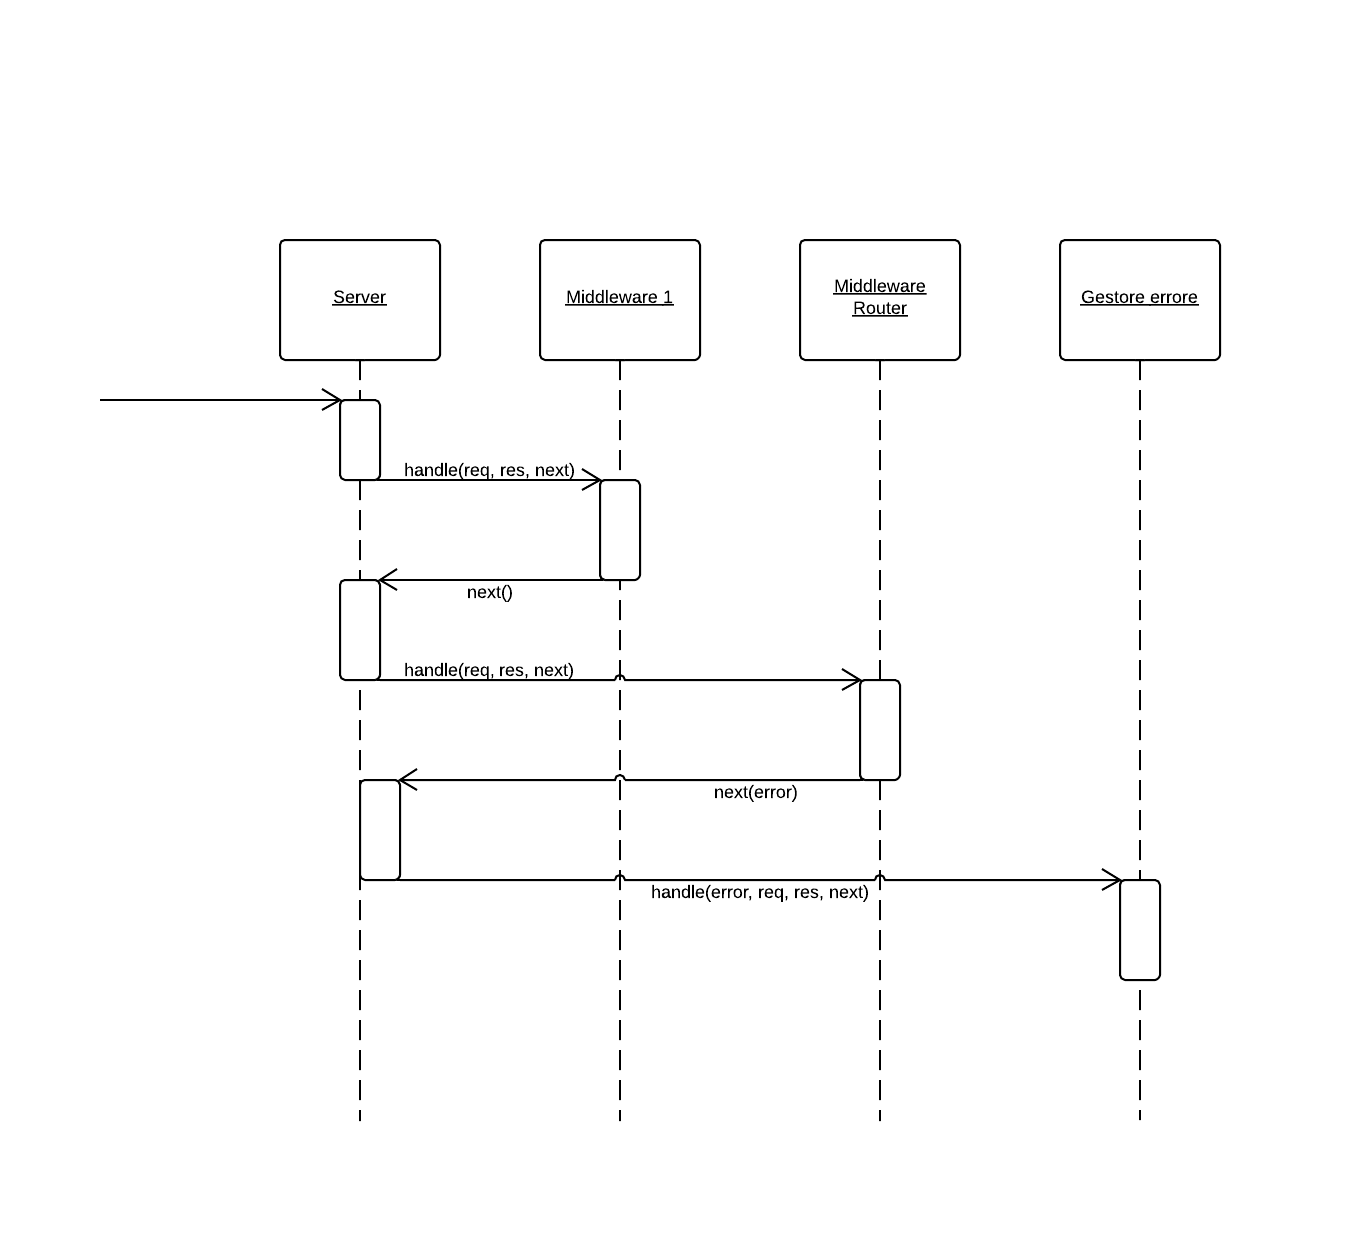
\includegraphics[scale=0.27]{scenari/Diagramma Gestione Richiesta.png}  
		\caption{Diagramma Gestione Richiesta}
	\end{center}  
\end{figure} 

Nel seguente diagramma viene mostrato il comportamento di routing, dove si intende che ogni controllore ha associato un'espressione regolare che specifica su quali richieste agisce. 
\begin{figure}[H]
	\begin{center} 
		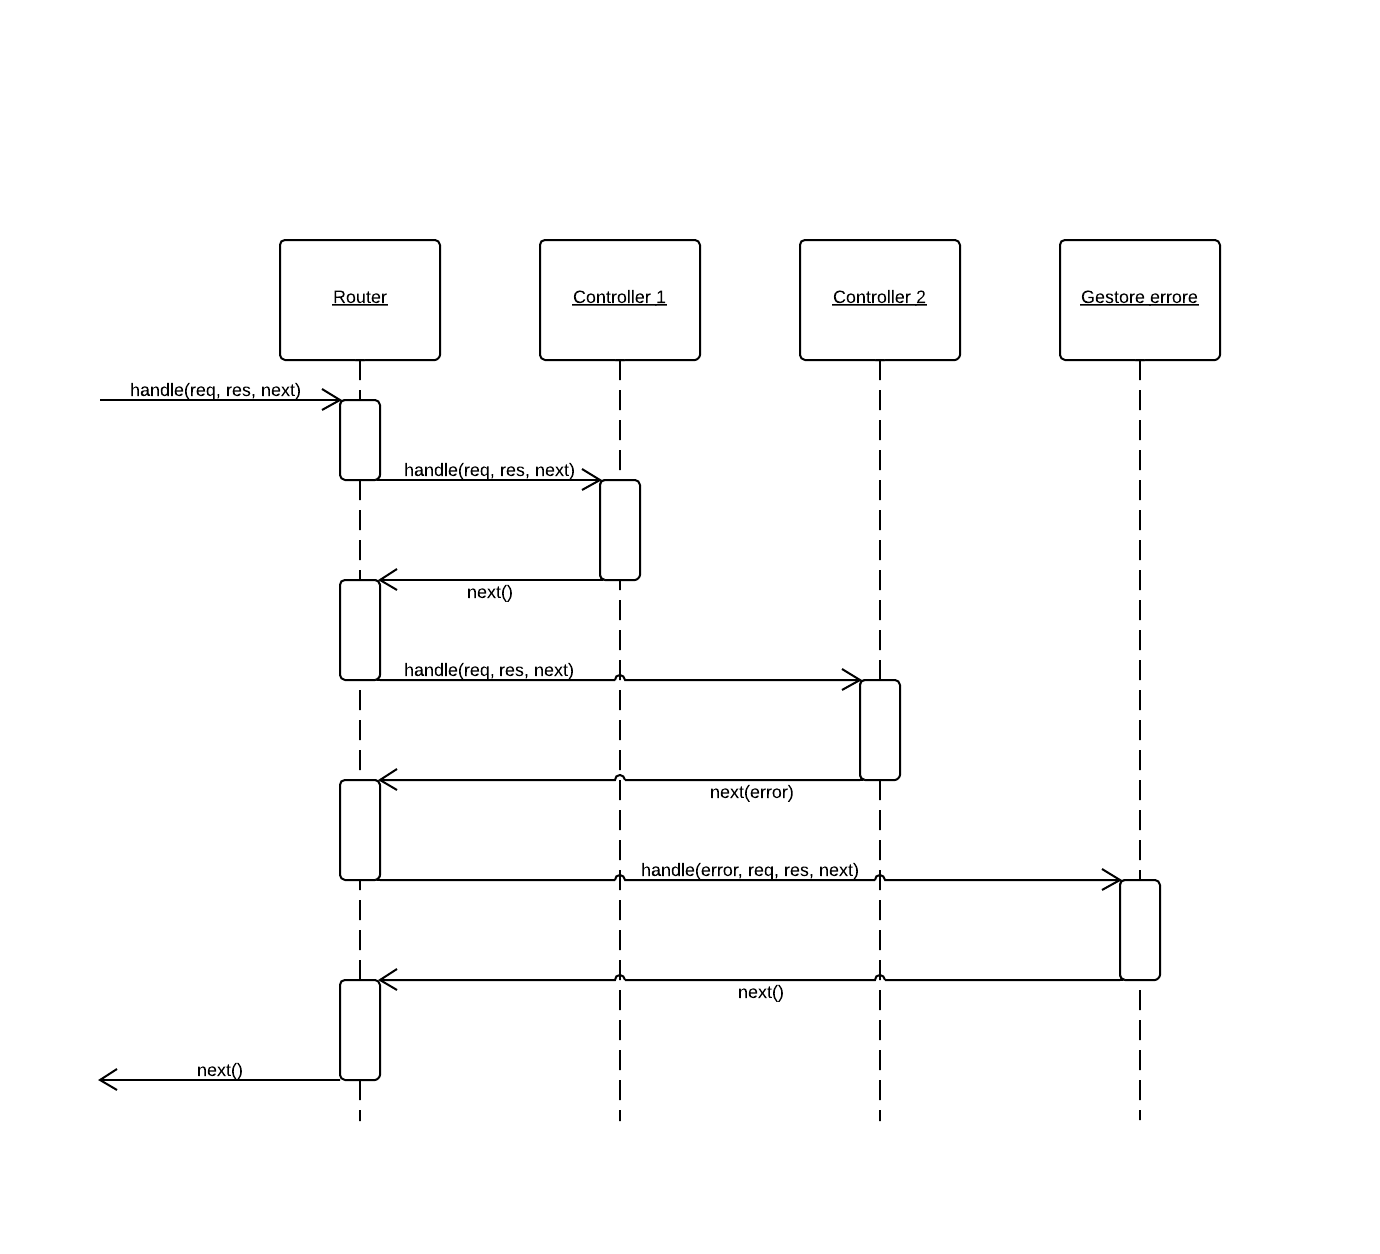
\includegraphics[scale=0.27]{scenari/Diagramma Routing Richiesta.png} 
		\caption{Diagramma Routing Richiesta}
	\end{center} 
\end{figure}

\subsection{Scenari}

\subsubsection{Fallimento vincolo ``utente autenticato''}
Per ogni richiesta bisogna verificare che il permesso dell'utente che l'ha chiesta, corrisponda al permesso che la risorsa necessita per poter essere effettuata. \\
Tale scenario rappresenta il fallimento di una richiesta richiedente come vincolo per poter essere effettuata che l'utente abbia un permesso di tipo ''utente autenticato'', dove la verifica dei permessi è gestita dal controller \emph{requireLogged} che manda un next(error) per il fallimento di tale vincolo al router il quale avrà compito di gestirlo.
\begin{figure}[H]
	\begin{center} 
		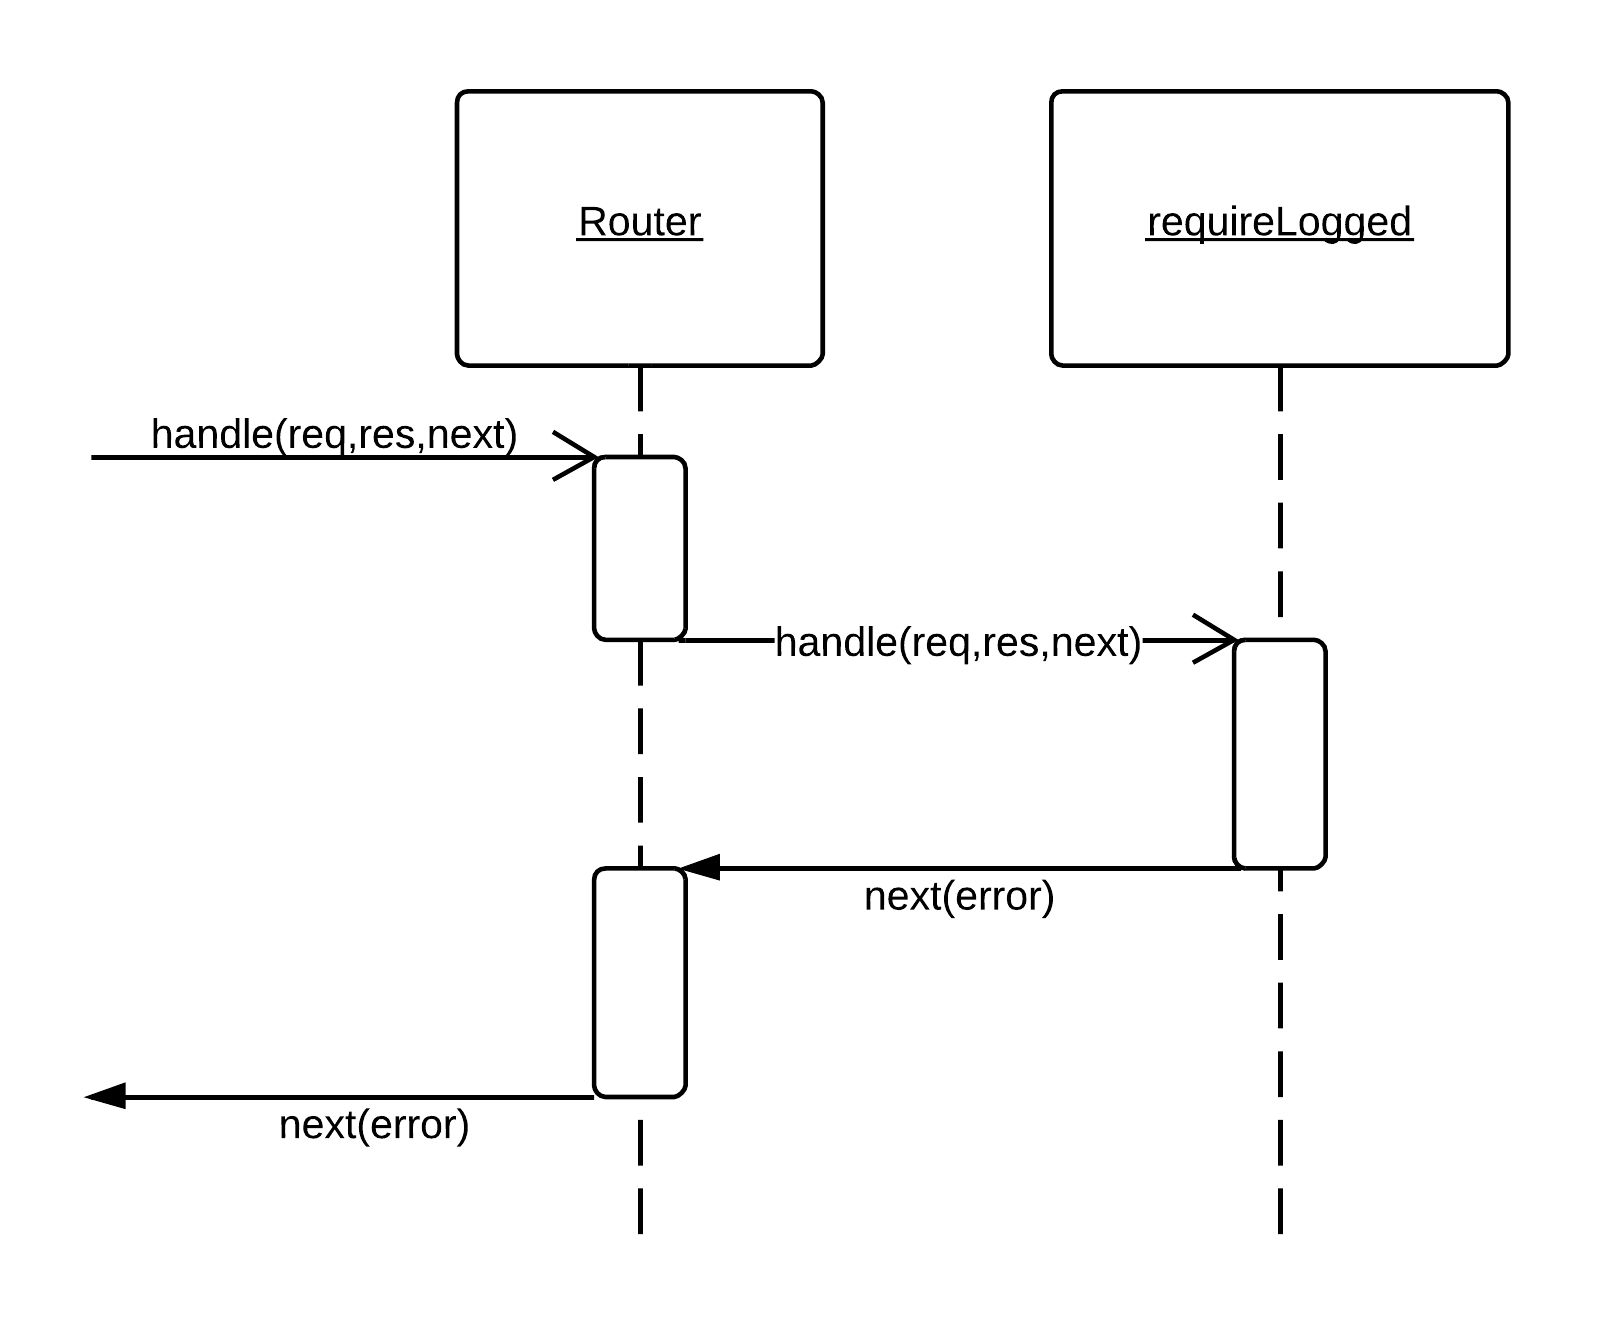
\includegraphics[scale=0.20]{scenari/requireLogged ERROR.png} 
		\caption{requireLogged ERROR}
	\end{center} 
\end{figure}

\subsubsection{Fallimento vincolo ``utente non autenticato''}
Il seguente diagramma di sequenza rappresenta lo scenario in cui fallisce la verifica del vincolo di permesso ''utente autenticato''.
La richiesta viene gestita da \emph{requireNotLogged} che verifica con esito negativo i permessi e rimanda un next(error) al router.
\begin{figure}[H]
	\begin{center} 
		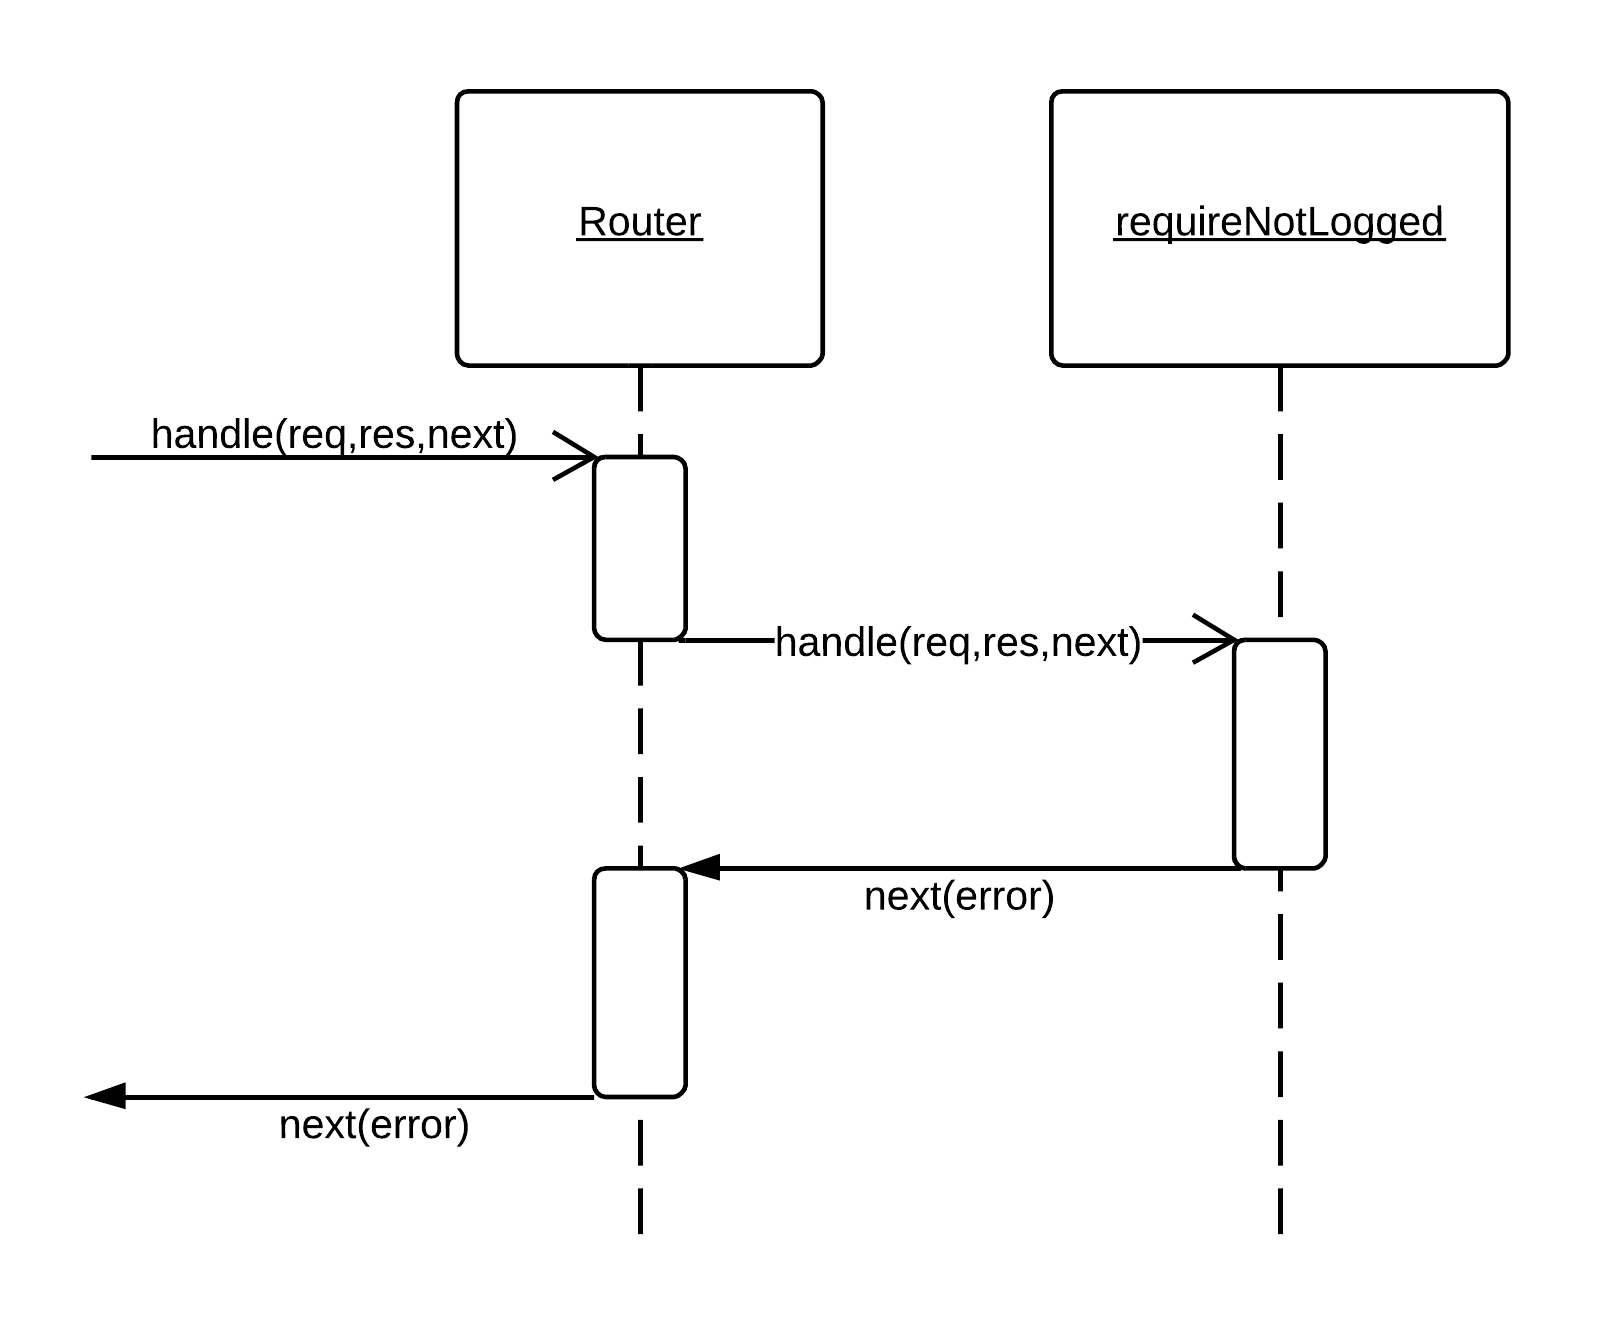
\includegraphics[scale=0.20]{scenari/requireNotLogged ERROR.png} 
		\caption{requireNotLogged ERROR}
	\end{center} 
\end{figure}

\subsubsection{Fallimento vincolo ``utente admin''}
Nel diagramma seguente viene rappresentato lo scenario in cui si richiedono permessi ''Admin'' per poter gestire la richiesta corrispondente e la verifica effettuata dal controller \emph{requireAdmin} fallisce. 
\begin{figure}[H]
	\begin{center} 
		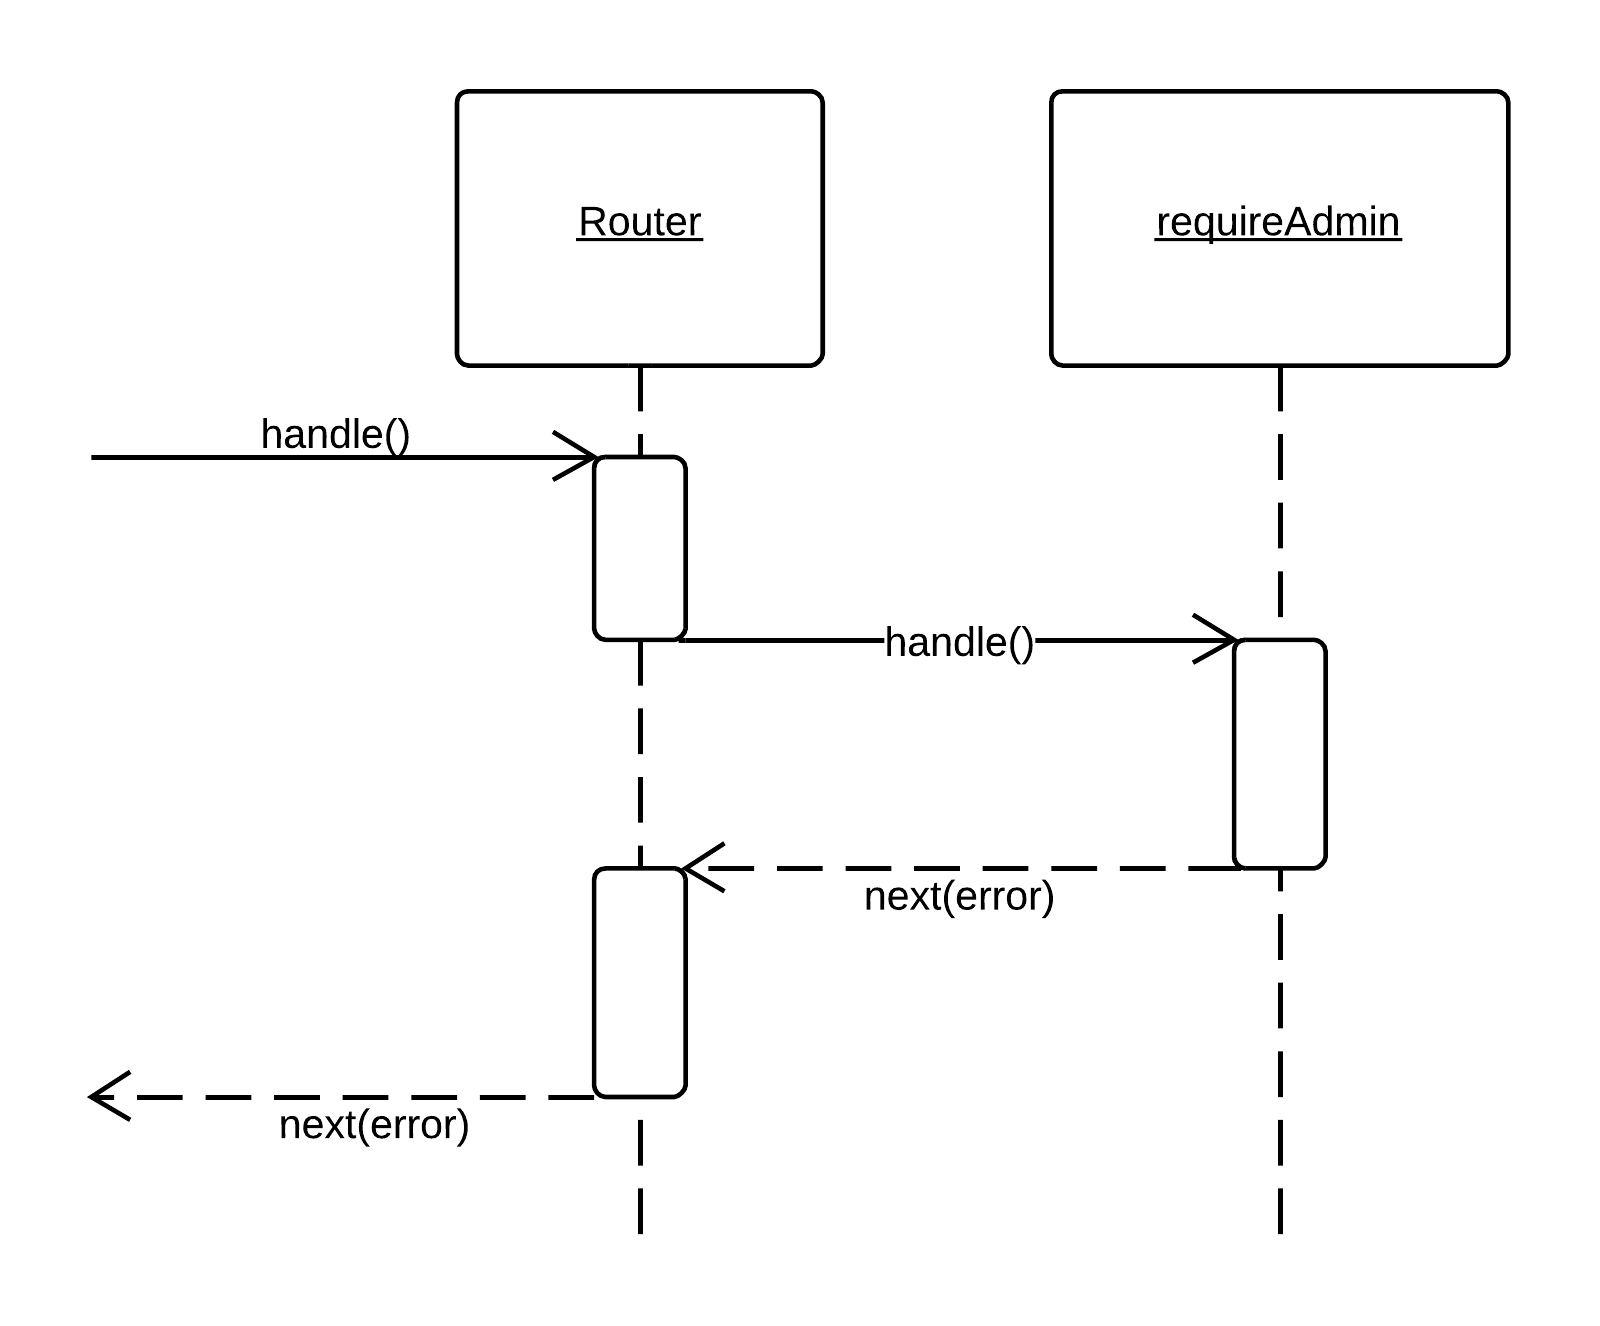
\includegraphics[scale=0.20]{scenari/requireAdmin ERROR.png} 
		\caption{requireAdmin ERROR}
	\end{center} 
\end{figure}


\subsubsection{Login POST} 
Il seguente scenario mostra la gestione di una richiesta POST per la risorsa di login, \emph{requireNotLogged} non risponde con errore, chiamando il successivo \glossario{middleware} \emph{login} che gestisce la verifica dei parametri e nell'opzione che questa fallisca, manda in risposta un next(error) che il router andrà a gestire.
\begin{figure}[H]
	\begin{center} 
		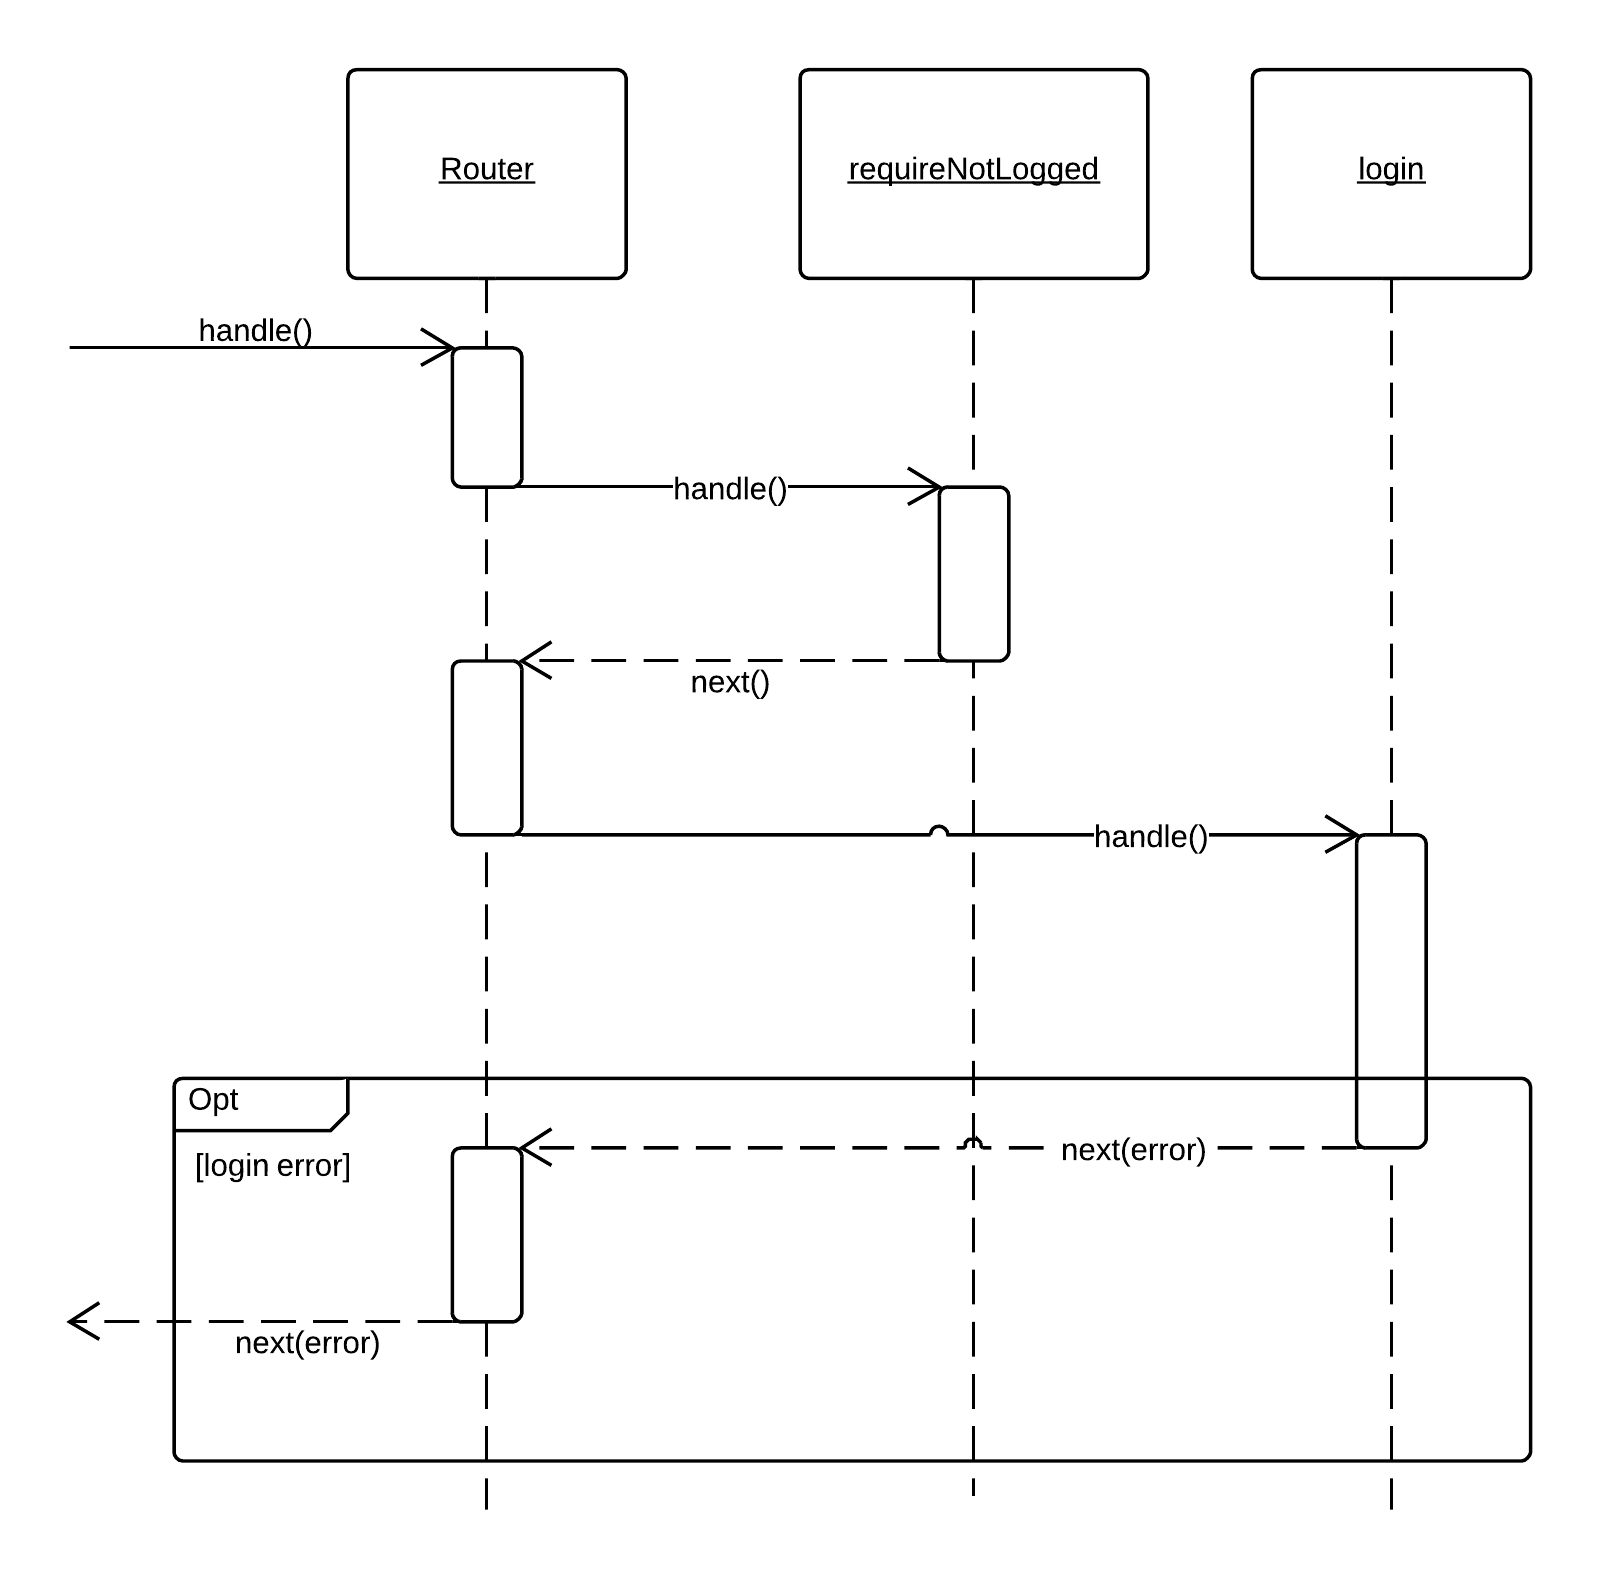
\includegraphics[scale=0.20]{scenari/login POST.png} 
		\caption{Login POST}
	\end{center} 
\end{figure} 

\subsubsection{Logout DELETE}
Il diagramma di sequenza mostra lo scenario di una richiesta DELETE per la risorsa login.
La verifica dei permessi in \emph{requireLogged} non fallisce, innescando la chiamata al successivo \glossario{middleware} \emph{logout} che gestisce l'eliminazione della risorsa.
\begin{figure}[H]
	\begin{center} 
		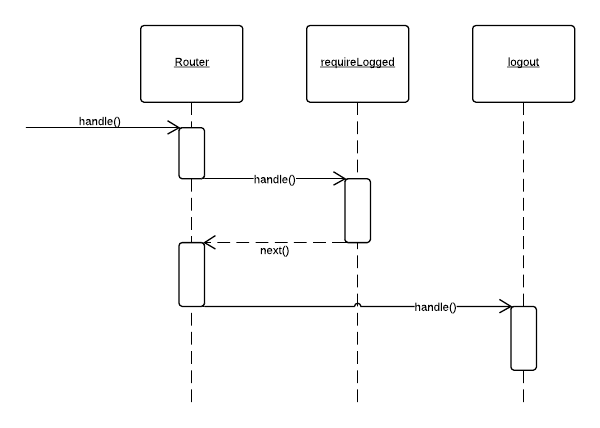
\includegraphics[scale=0.20]{scenari/logout DELETE.png} 
		\caption{Logout DELETE}
	\end{center} 
\end{figure}

\subsubsection{Profile GET} 
Il seguente diagramma rappresenta lo scenario di una richiesta GET per ottenere la risorsa Profile, la verifica dei permessi non fallisce e la richiesta viene gestita da \emph{getProfile}.
\begin{figure}[H]
	\begin{center} 
		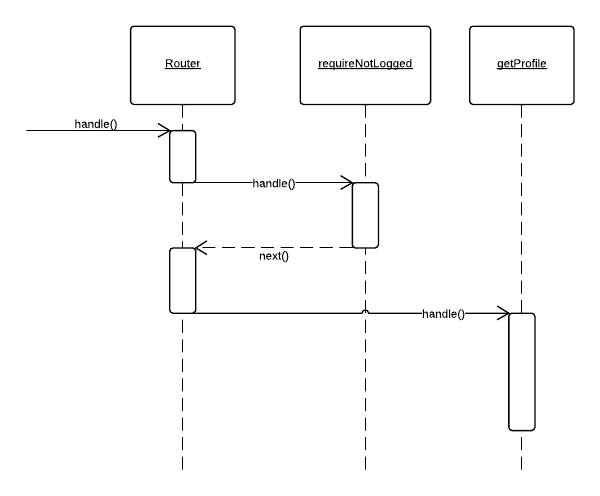
\includegraphics[scale=0.20]{scenari/Profile GET.png} 
		\caption{Profile GET}
	\end{center} 
\end{figure}

\subsubsection{Profile PUT} 
Viene rappresentato lo scenario di una richiesta PUT per la risorsa Profile, il \emph{requireLogged} non ritorna un errore, chiamando il successivo \glossario{middleware} \emph{editProfile} che gestisce la richiesta di modifica dei dati del profilo.
\begin{figure}[H]
	\begin{center} 
		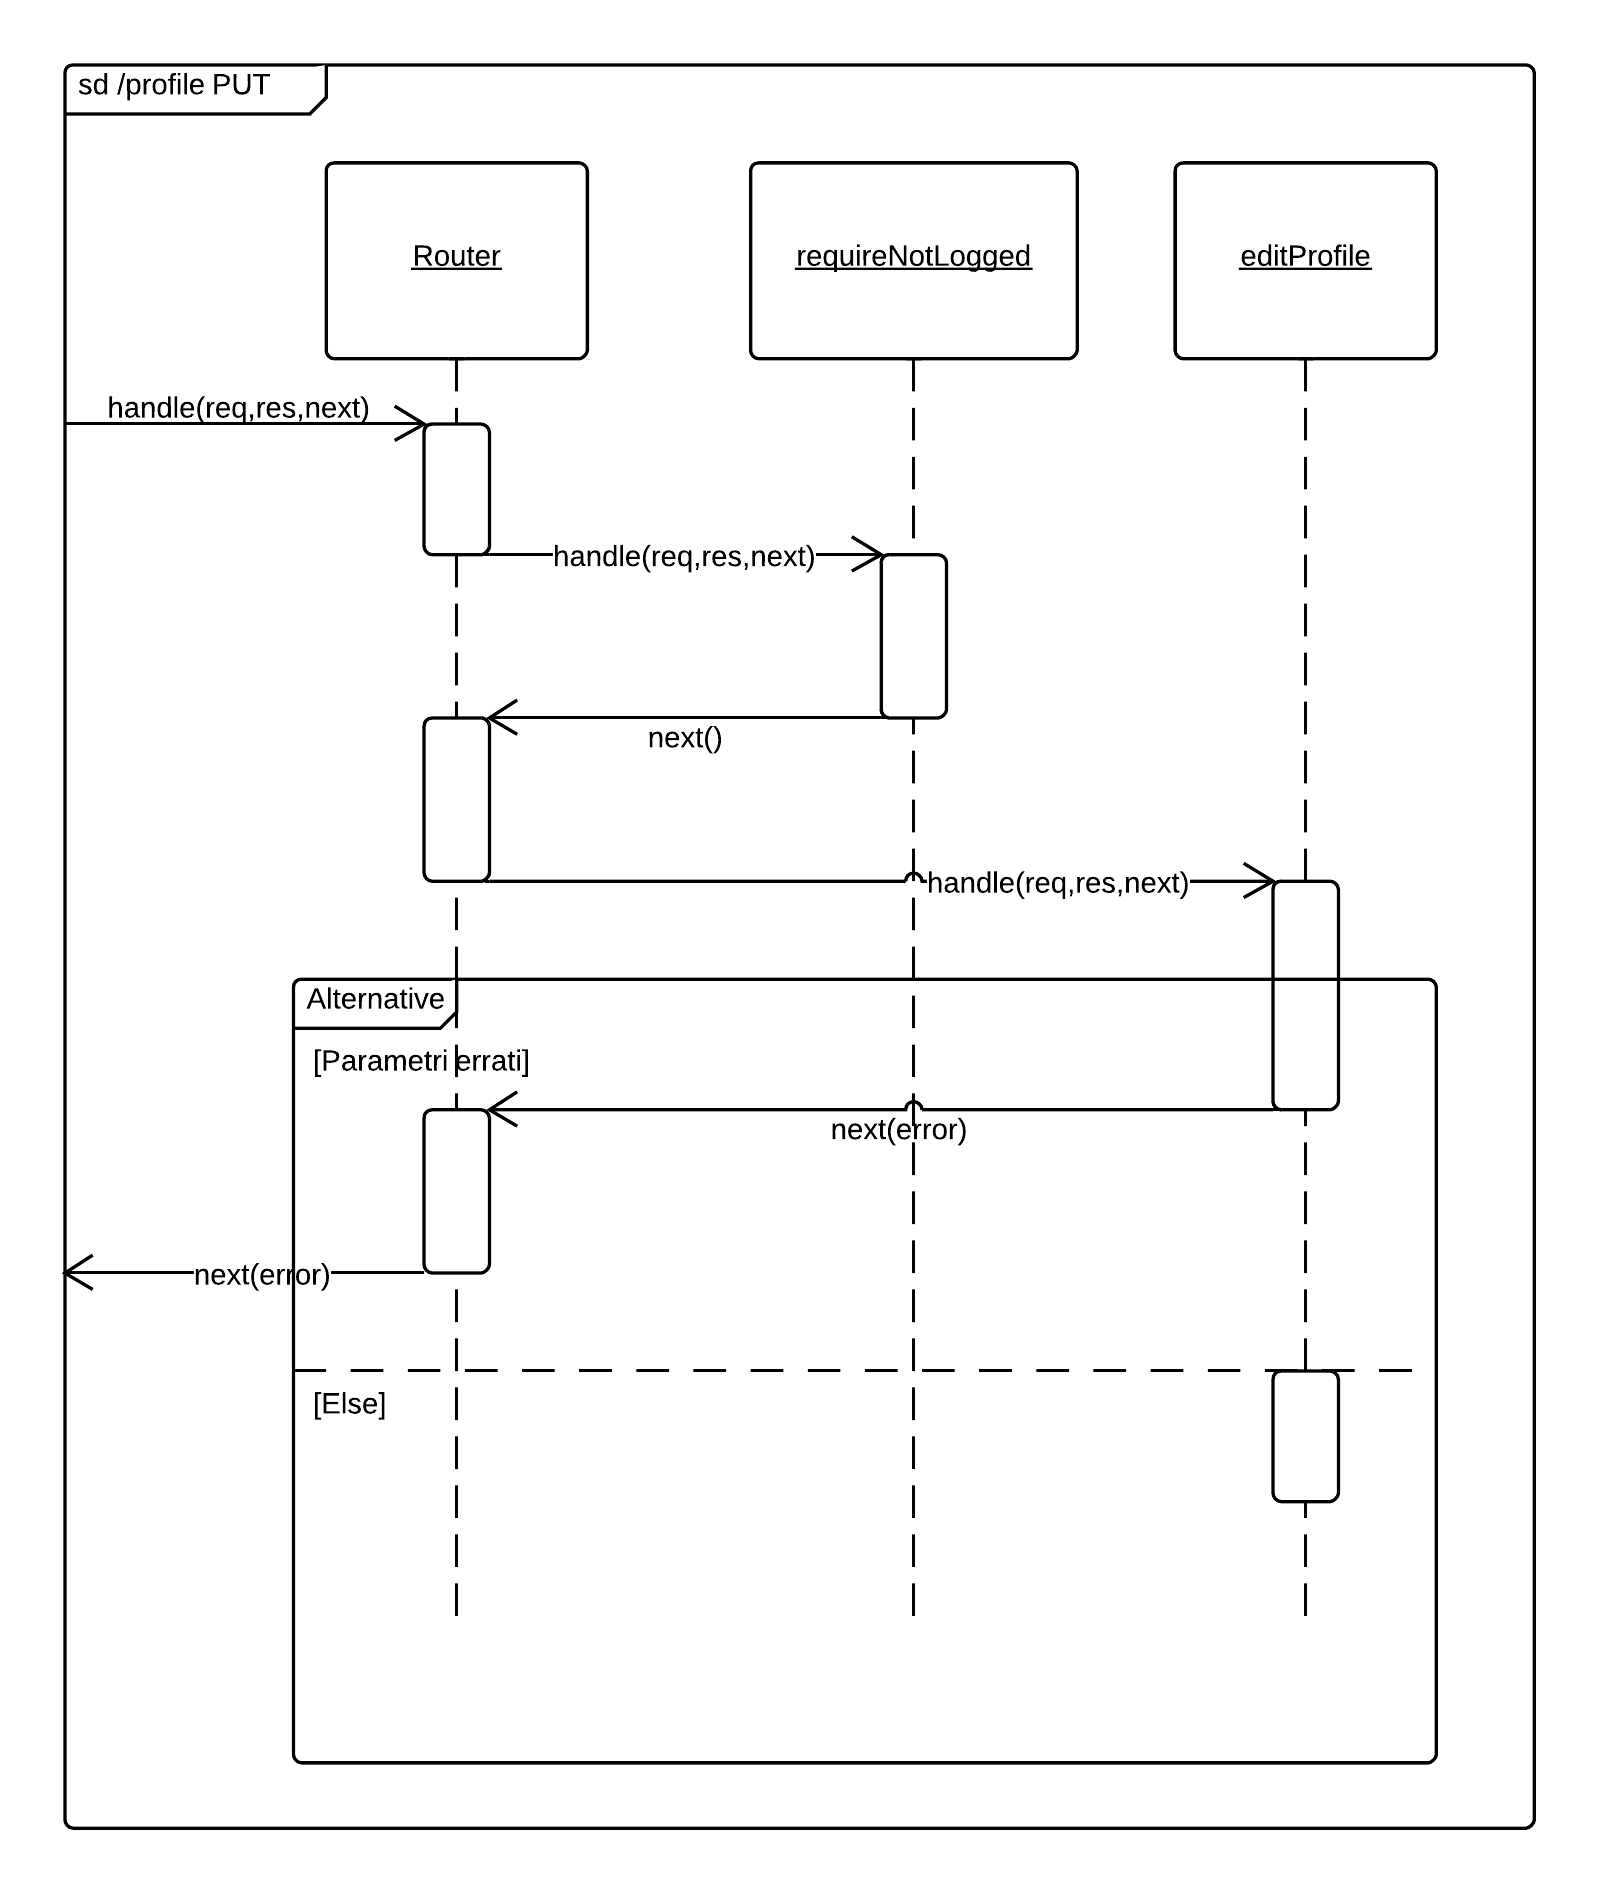
\includegraphics[scale=0.20]{scenari/Profile PUT.png} 
		\caption{Profile PUT}
	\end{center} 
\end{figure}

\subsubsection{Password Forgot POST} 
Viene rappresentato lo scenario di una richiesta POST per la risorsa password forgot, il \emph{requireNotLogged} non risponde errore e il controllo passa a \emph{requirePasswordReset} che gestisce la richiesta.
\begin{figure}[H]
	\begin{center} 
		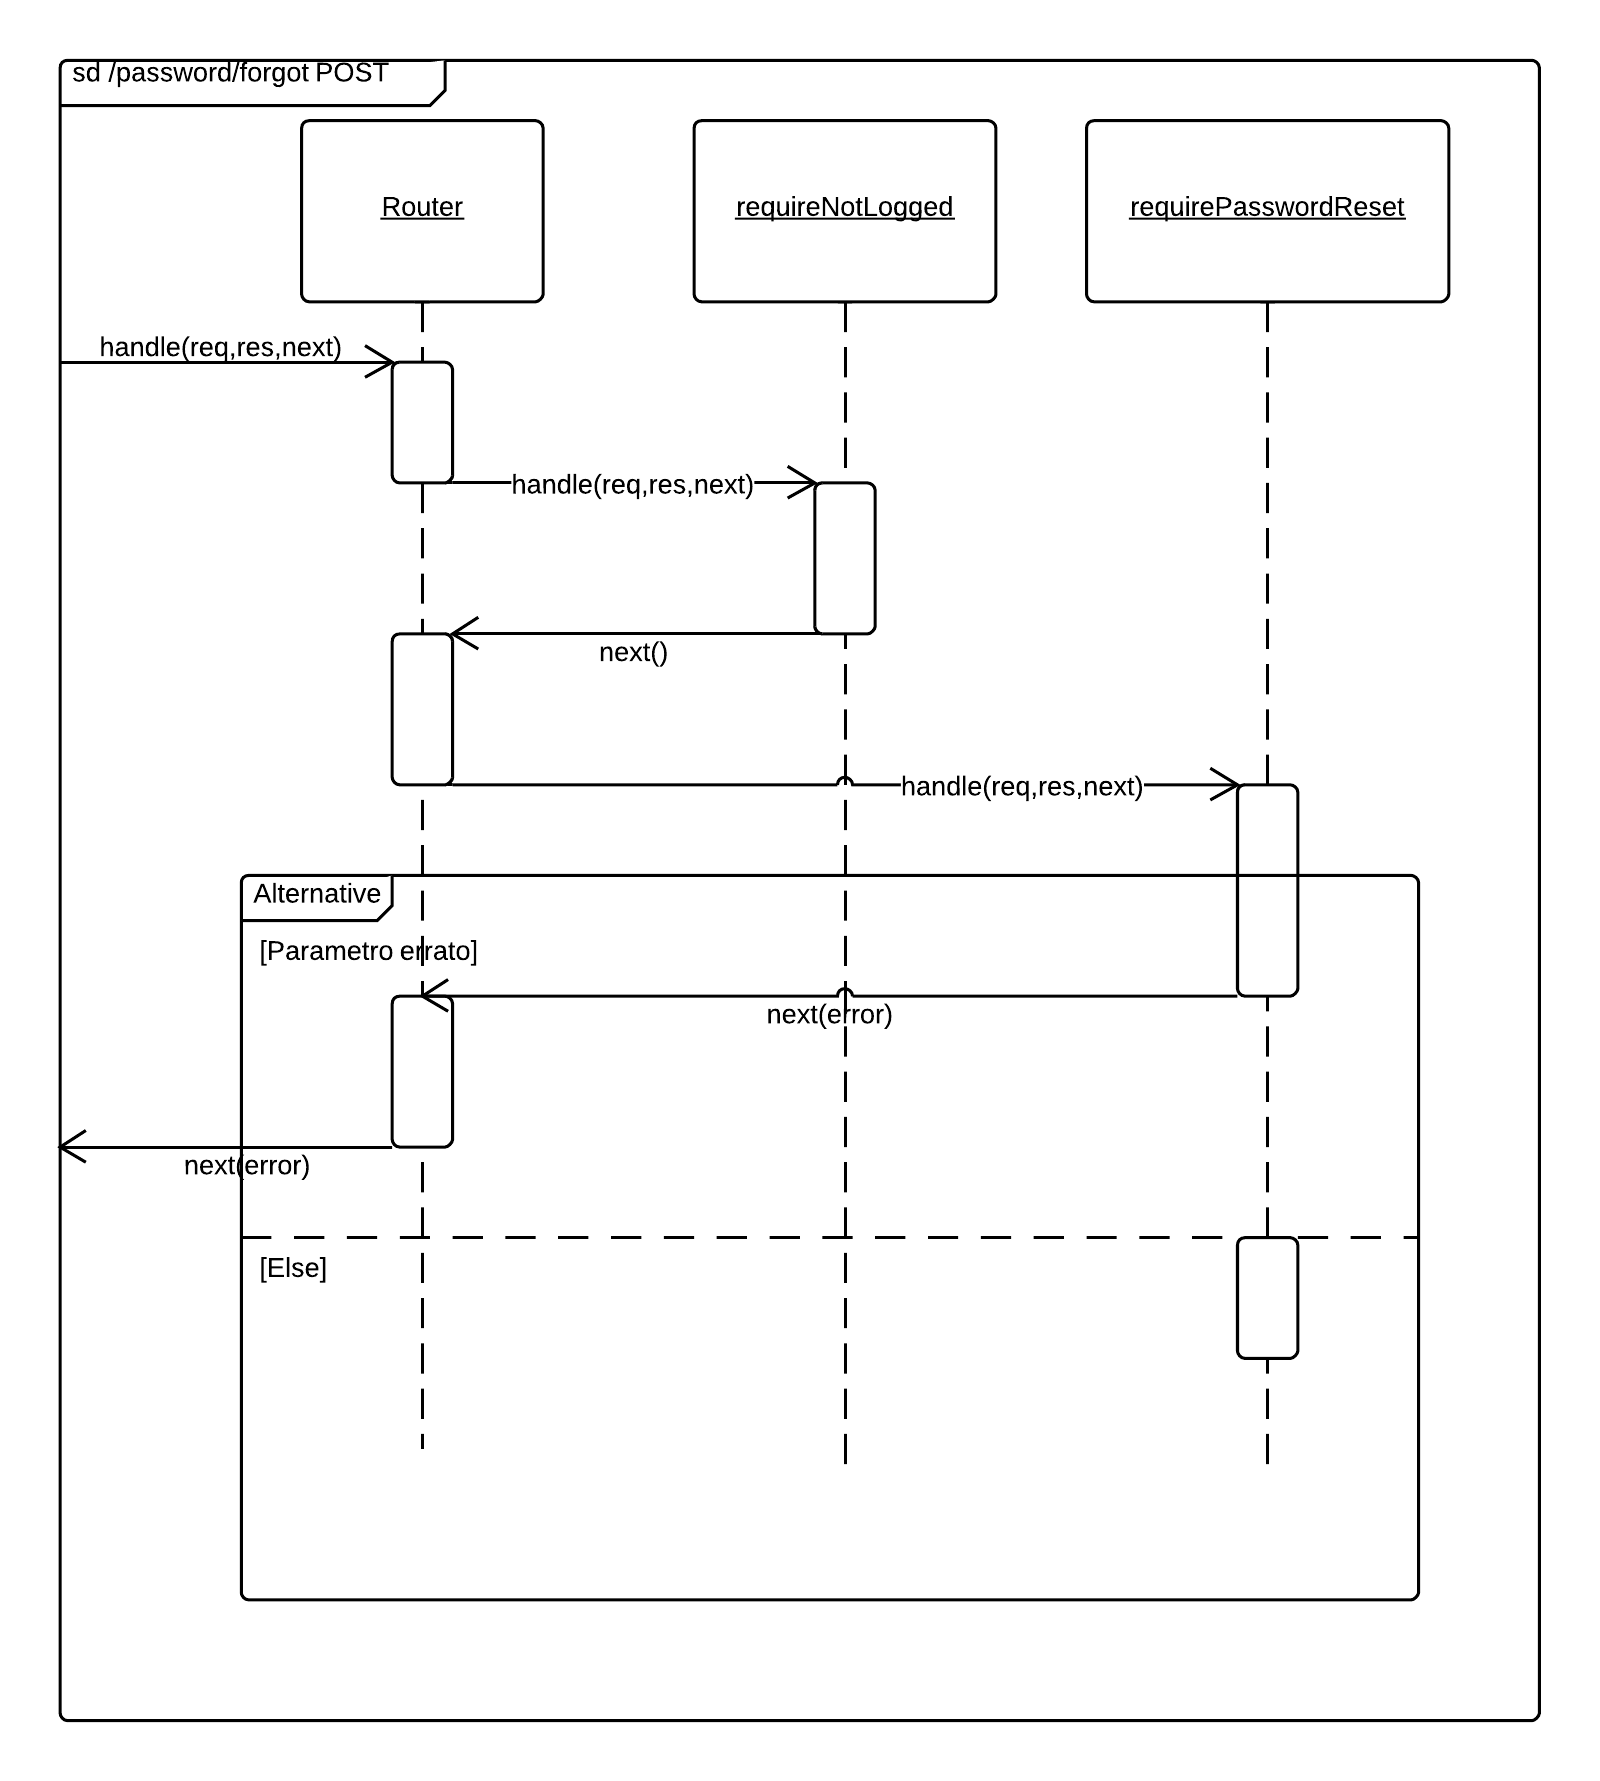
\includegraphics[scale=0.20]{scenari/Password Forgot POST.png} 
		\caption{Password Forgot POST}
	\end{center} 
\end{figure}

\subsubsection{Users GET}
Viene rappresentato nel seguente diagramma di sequenza lo scenario di una richiesta GET per la risorsa user, \emph{requireAdmin} non fallisce ed il controllo viene passato a \emph{getUsers} che gestisce la richiesta.
\begin{figure}[H]
	\begin{center} 
		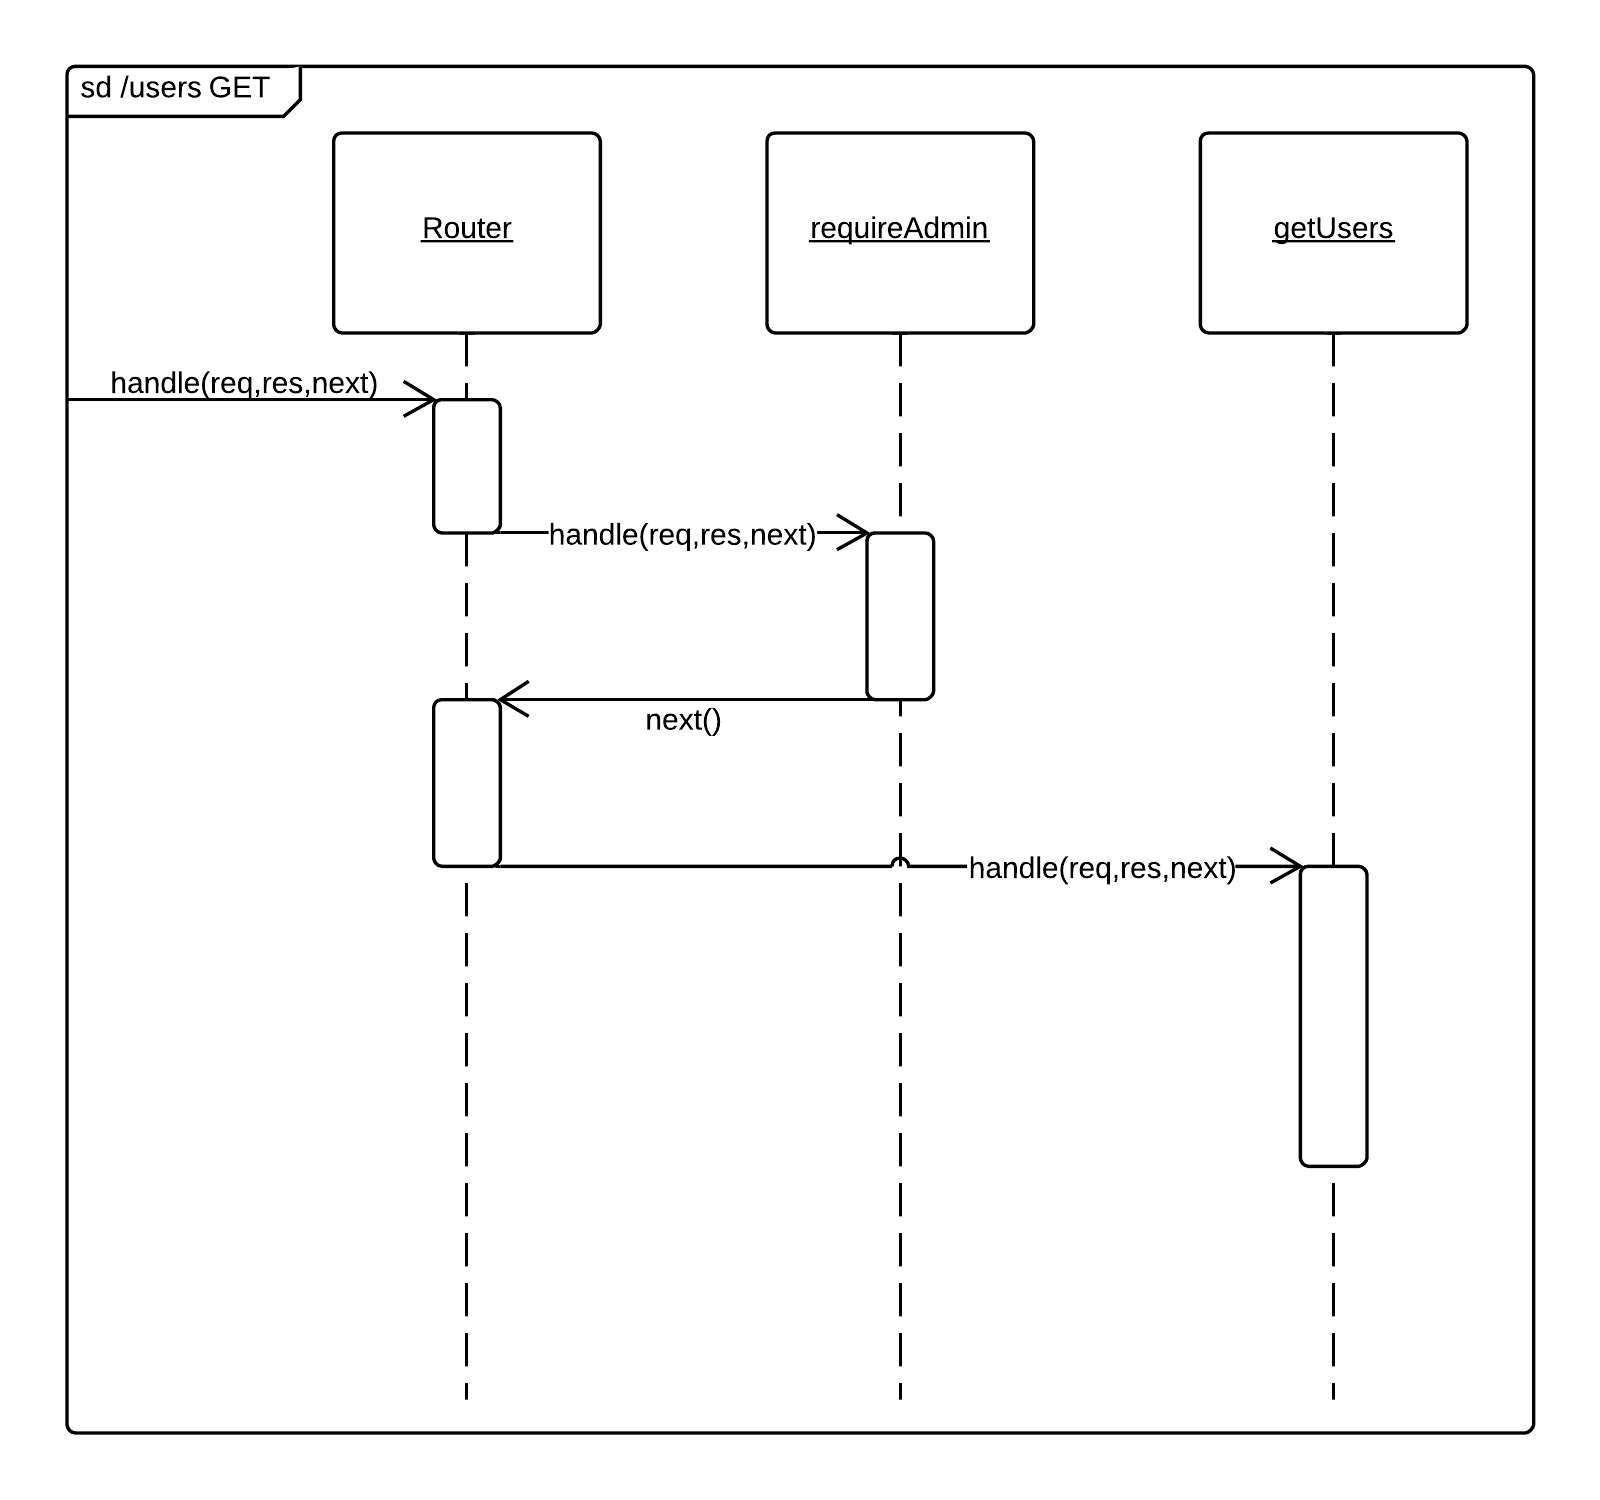
\includegraphics[scale=0.20]{scenari/Users GET.png} 
		\caption{Users GET}
	\end{center} 
\end{figure}

\subsubsection{Users POST} 
Il seguente diagramma di sequenza rappresenta lo scenario di una richiesta POST per la risorsa user, la verifica di \emph{requireLogged} dei permessi utente non fallisce e viene passato il controllo a \emph{createUser} che gestisce la richiesta di creazione di un nuovo user.
\begin{figure}[H]
	\begin{center} 
		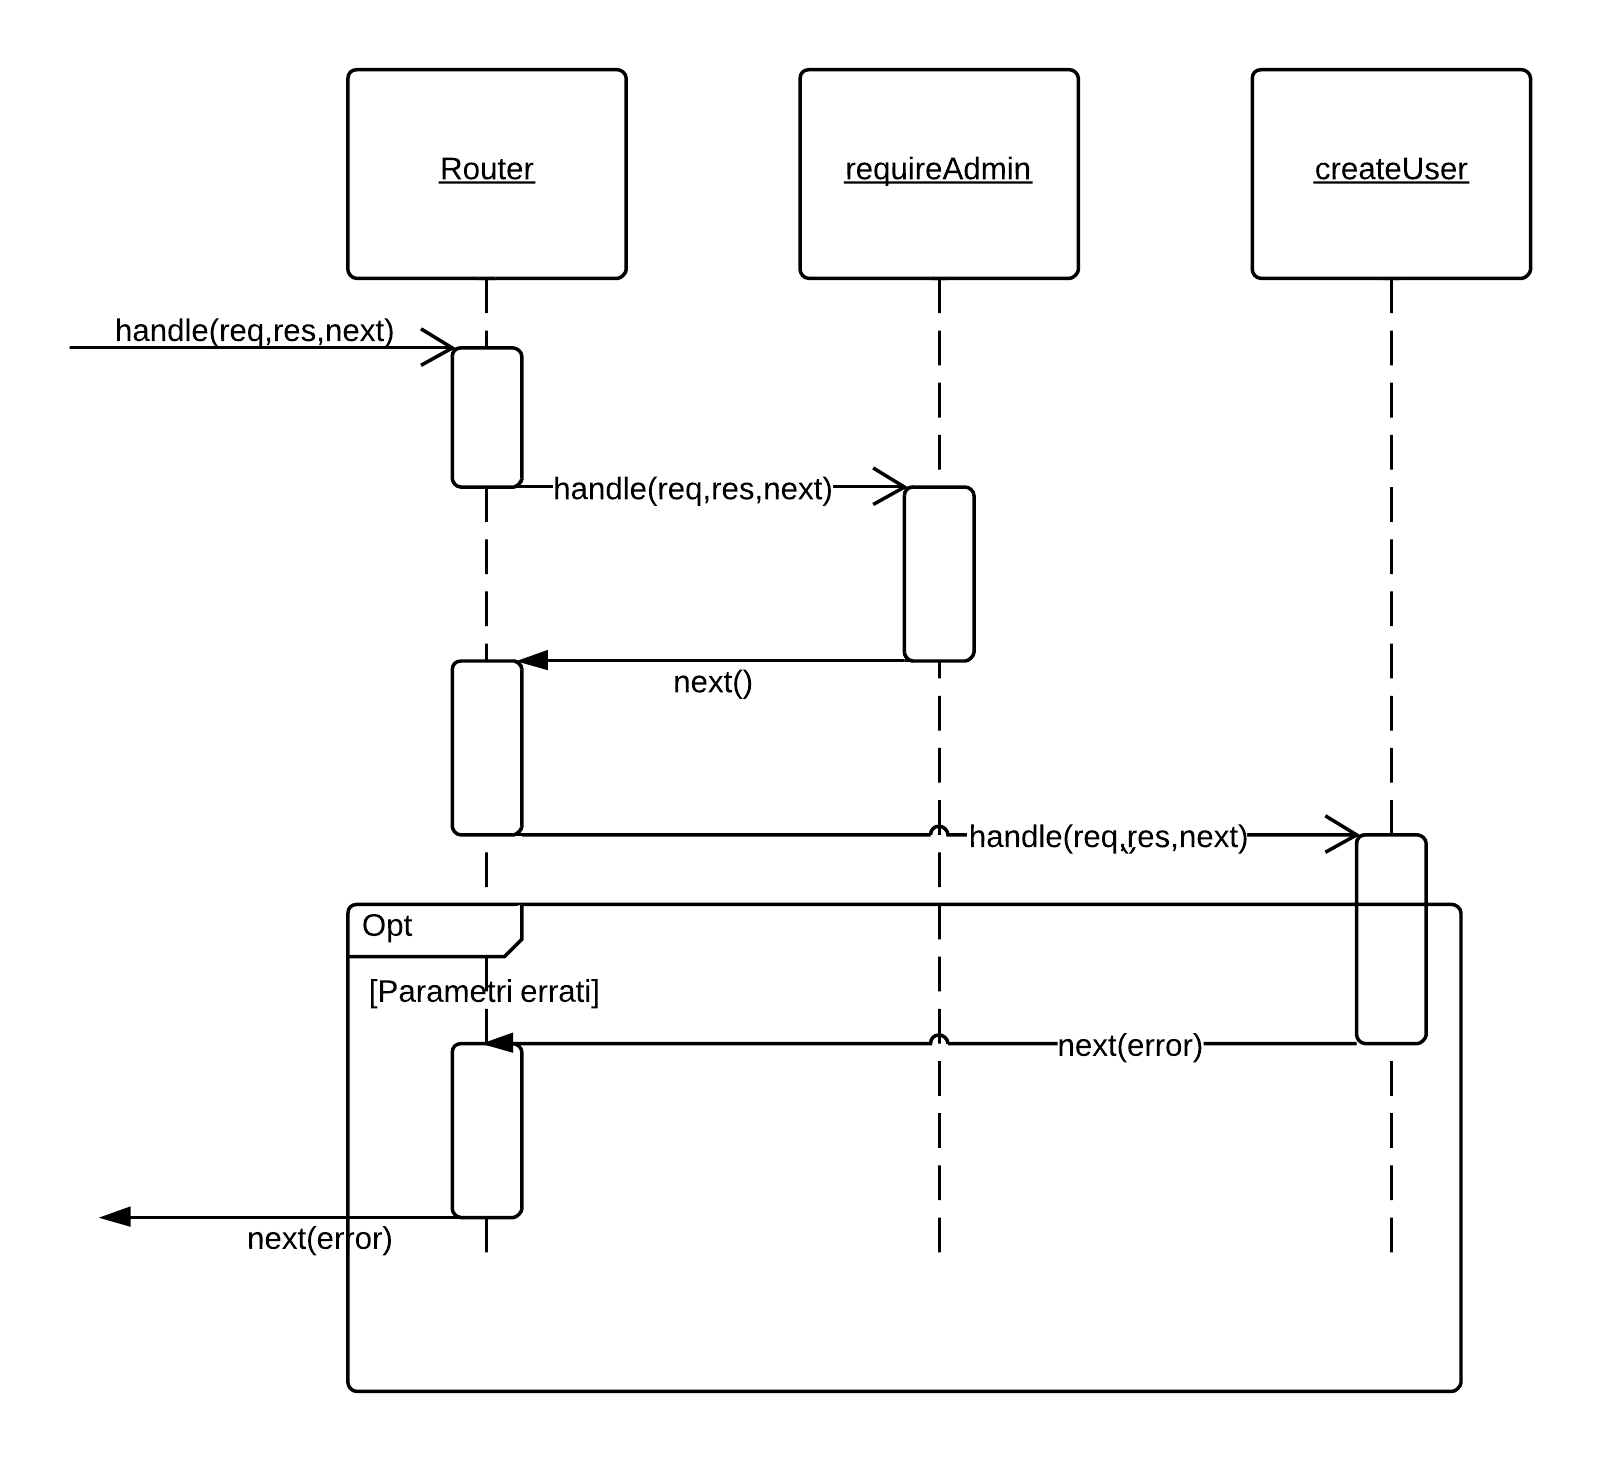
\includegraphics[scale=0.20]{scenari/Users POST.png} 
		\caption{Users POST}
	\end{center} 
\end{figure}

\subsubsection{Users Id GET} 
Lo scenario rappresenta una richiesta GET di una risorsa User id, vengono verificati i permessi attraverso \emph{requireAdmin} che passa il controllo a \emph{getUser} dandogli come attributo l'id dell'user da restituire.
\begin{figure}[H]
	\begin{center} 
		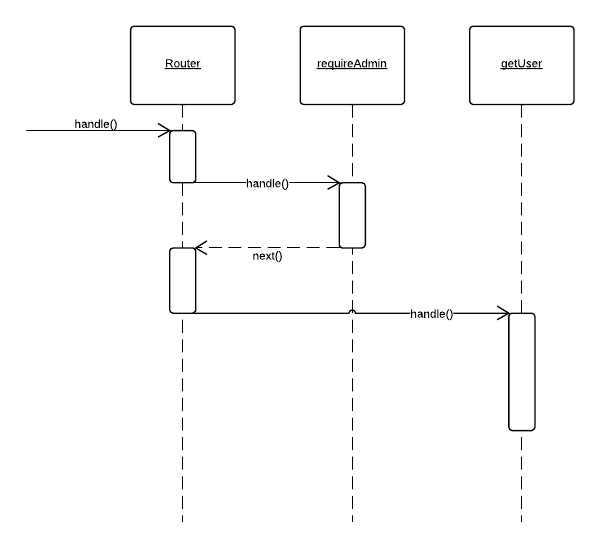
\includegraphics[scale=0.20]{scenari/Users Id GET.png} 
		\caption{Users Id GET}
	\end{center} 
\end{figure}

\subsubsection{Users Id PUT} 
Nel seguente diagramma di sequenza viene rappresentato lo scenario di una richiesta PUT per la risorsa User id nel quale \emph{requireAdmin} non restituisce un errore e passa il controllo a \emph{editUser} che gestisce la richiesta di modifica dati dell'user corrispondente all'userId che gli è stato passato come attributo.
\emph{EditUser} verifica inoltre che l'userId passatogli come attributo non corrisponda all'id dello stesso user che ha effettuato la richiesta o corrisponda ad un id di un superAdmin, altrimenti risponderà con un errore.
\begin{figure}[H]
	\begin{center} 
		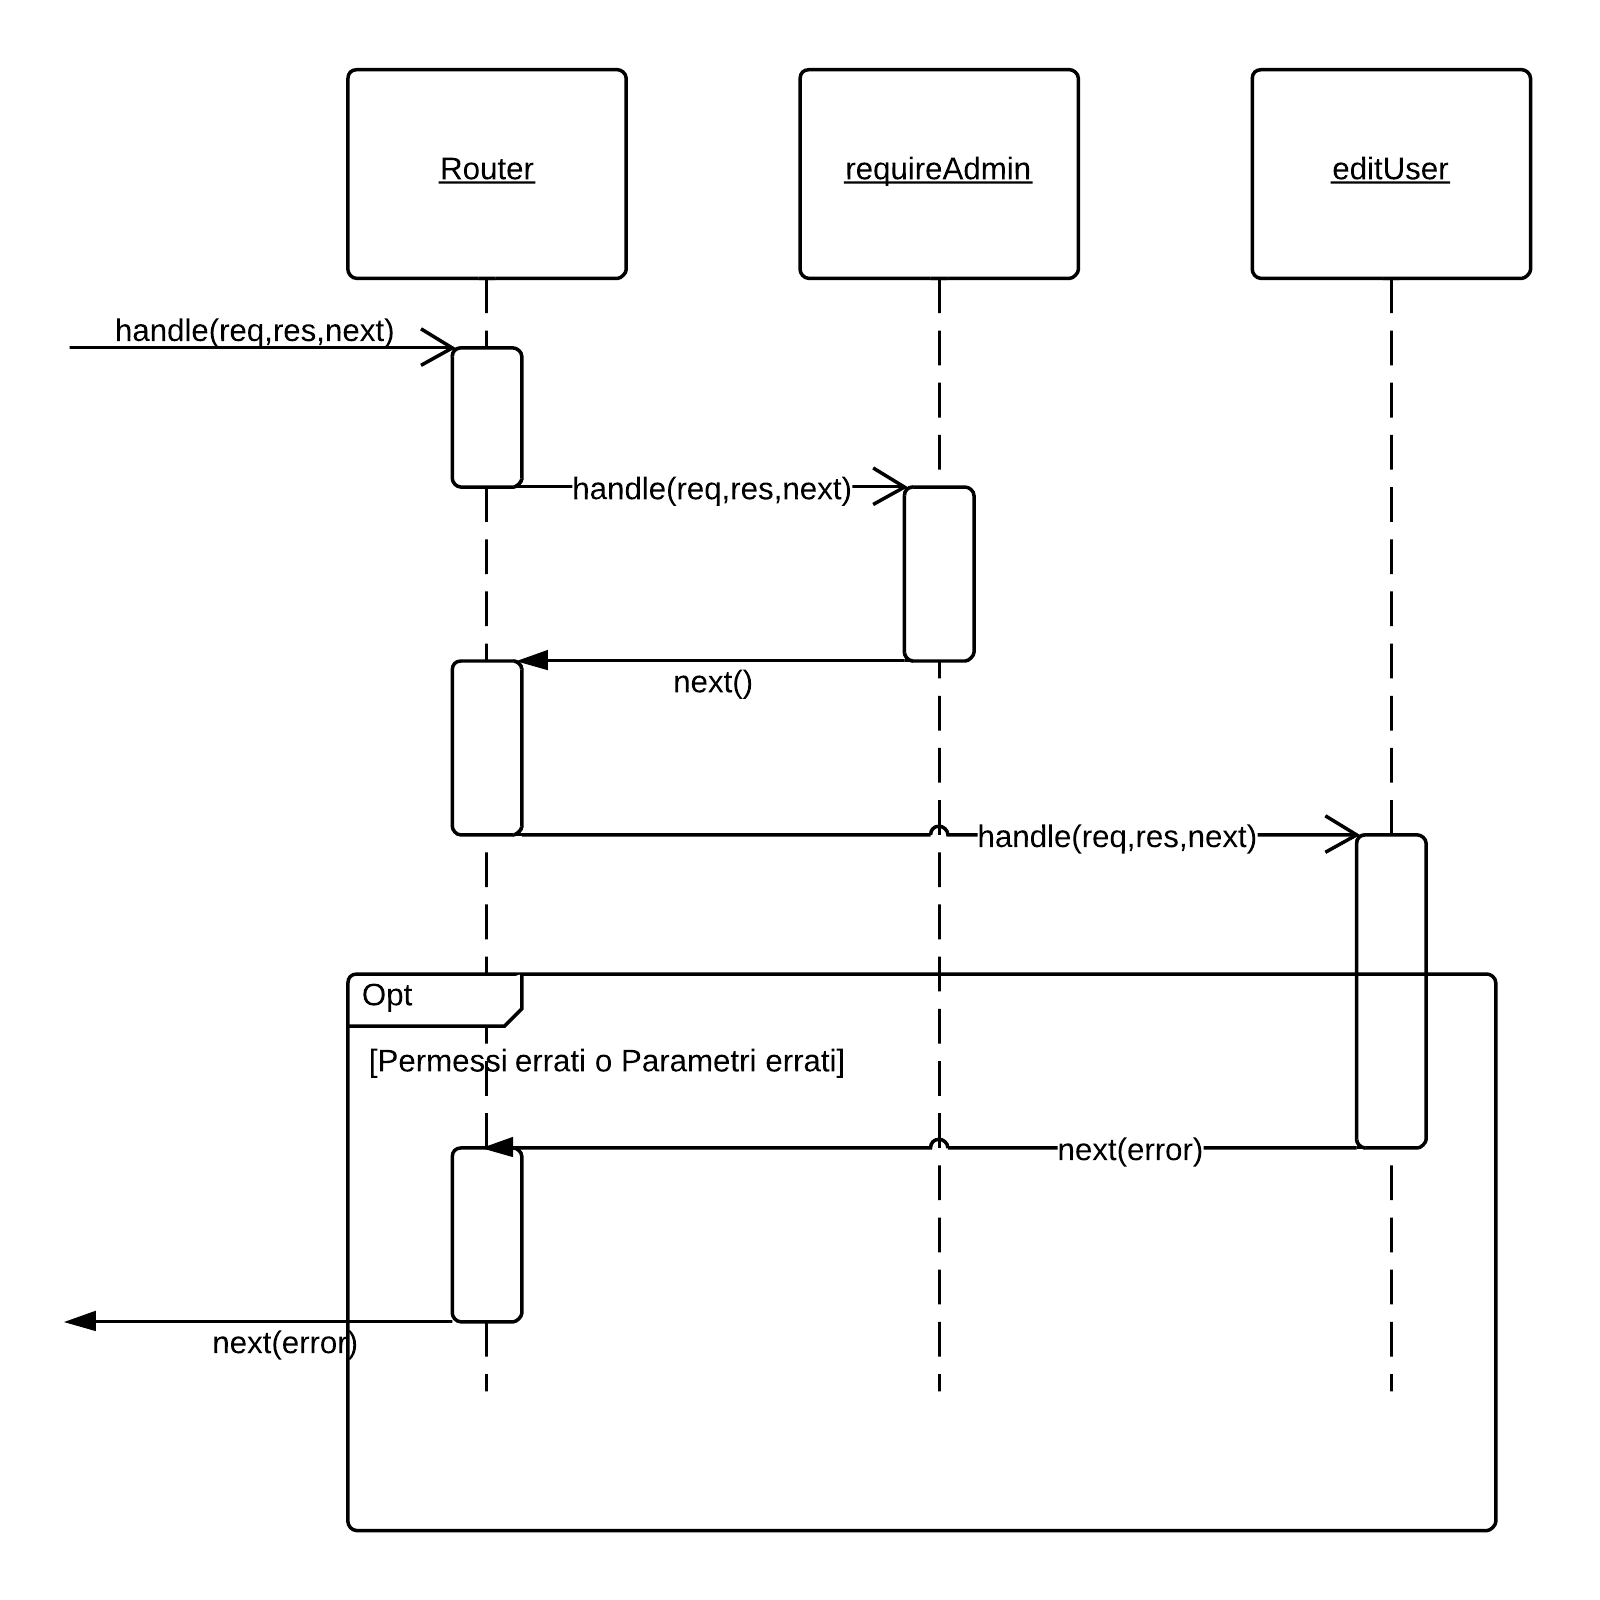
\includegraphics[scale=0.20]{scenari/Users Id PUT.png} 
		\caption{Users Id POST}
	\end{center} 
\end{figure}

\subsubsection{Users Id DELETE} 
Il diagramma di sequenza rappresenta lo scenario di una richiesta DELETE per la risorsa user id, \emph{requireAdmin} non restituisce un errore e la richiesta viene gestita da \emph{deleteUser} per procede con l'eliminazione dell'user cui id gli è stato passato come attributo.
Nell'opzione che l'id passatogli corrisponda all'id dell'utente che ha effettuato la richiesta o ad un id di un superAdmin, \emph{deleteUser} restituisce un next(error).
\begin{figure}[H]
	\begin{center} 
		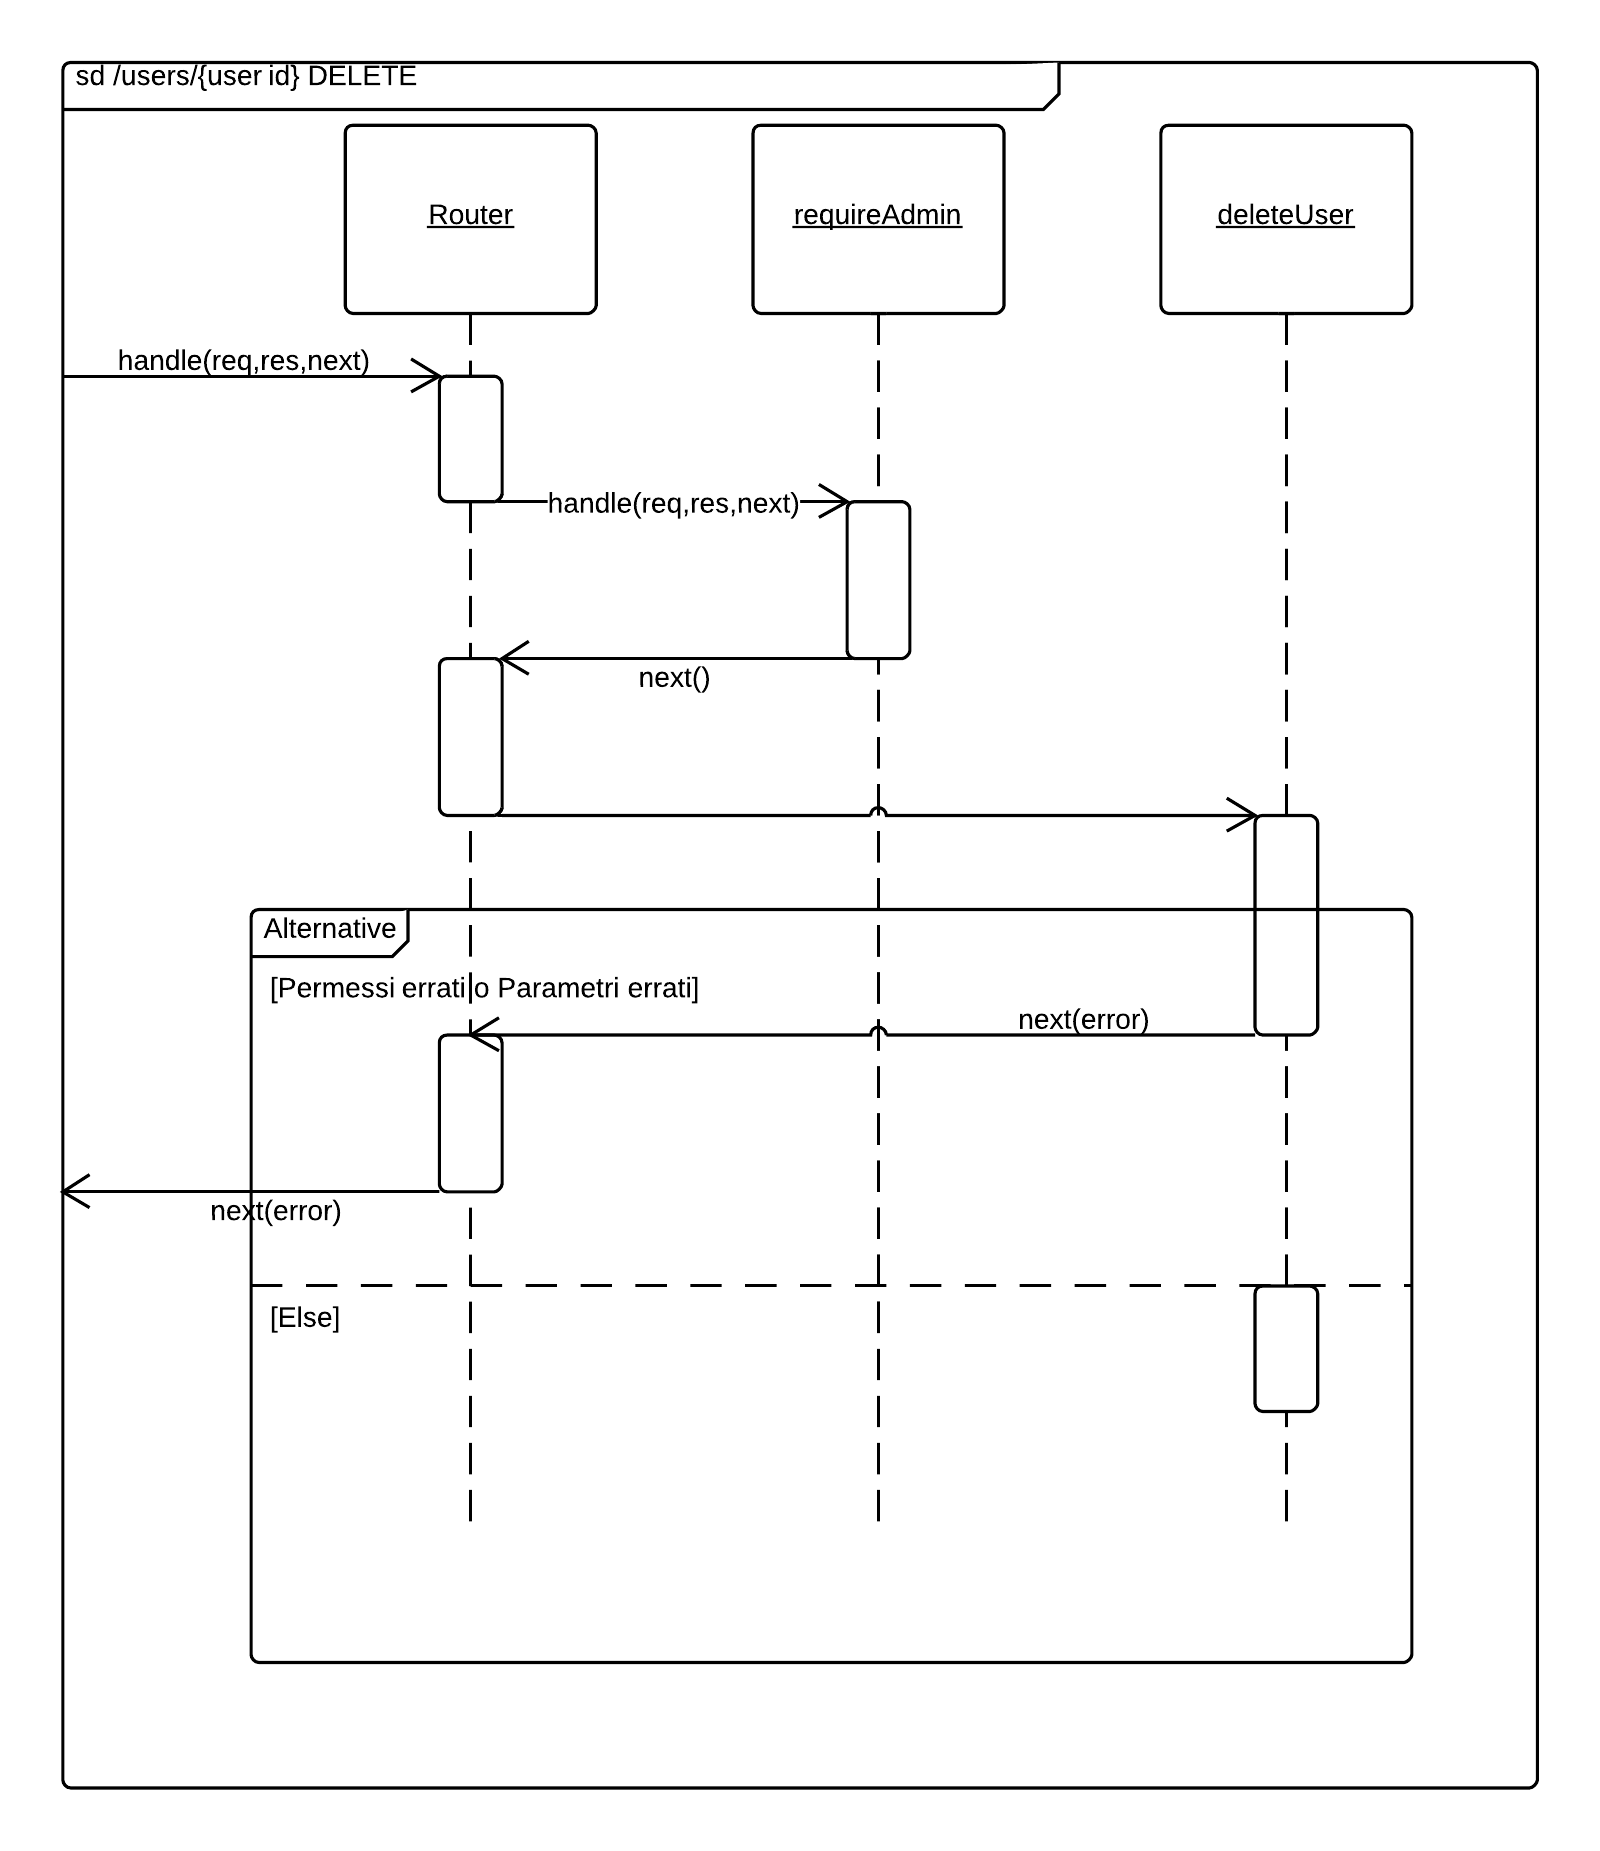
\includegraphics[scale=0.20]{scenari/Users Id DELETE.png} 
		\caption{Users Id DELETE}
	\end{center} 
\end{figure}

\subsubsection{Collection GET} 
Il diagramma seguente rappresenta lo scenario di una richiesta GET per la risorsa collection, il controller \emph{requireLogged} innescherà la chiamata del successivo controller \emph{listCollection} che gestirà la richiesta di restituzione della lista di \glossario{Collection}.
\begin{figure}[H]
	\begin{center} 
		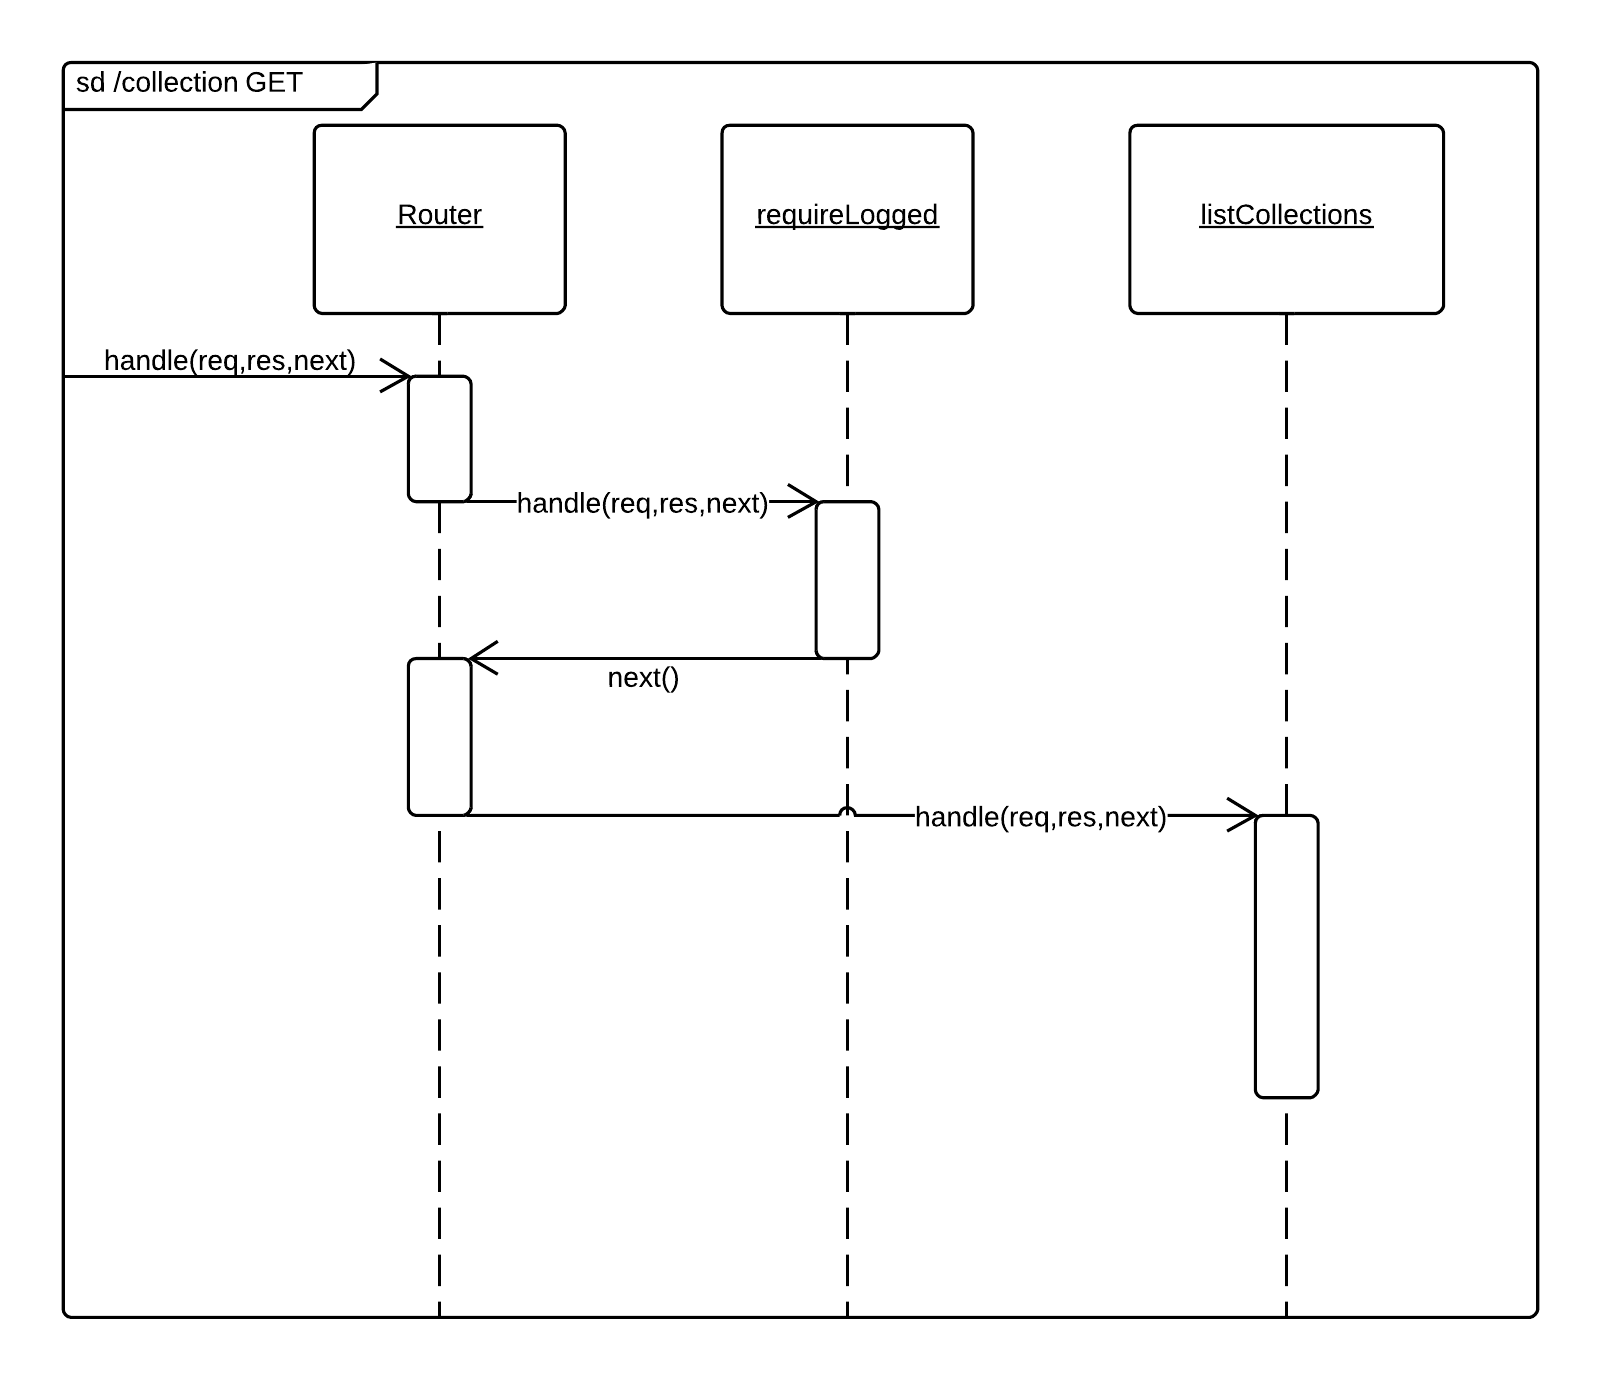
\includegraphics[scale=0.20]{scenari/Collection GET.png} 
		\caption{Collection GET}
	\end{center} 
\end{figure}

\subsubsection{Collection Name GET} 
Il diagramma seguente rappresenta lo scenario di una richiesta GET per la risorsa collection Name, il controller \emph{requireLogged} innescherà la chiamata del successivo controller \emph{indexPage} al quale verrà passato come parametro l'id della \glossario{Collection} per la restituzione dell'index page corrispondente.
\begin{figure}[H]
	\begin{center} 
		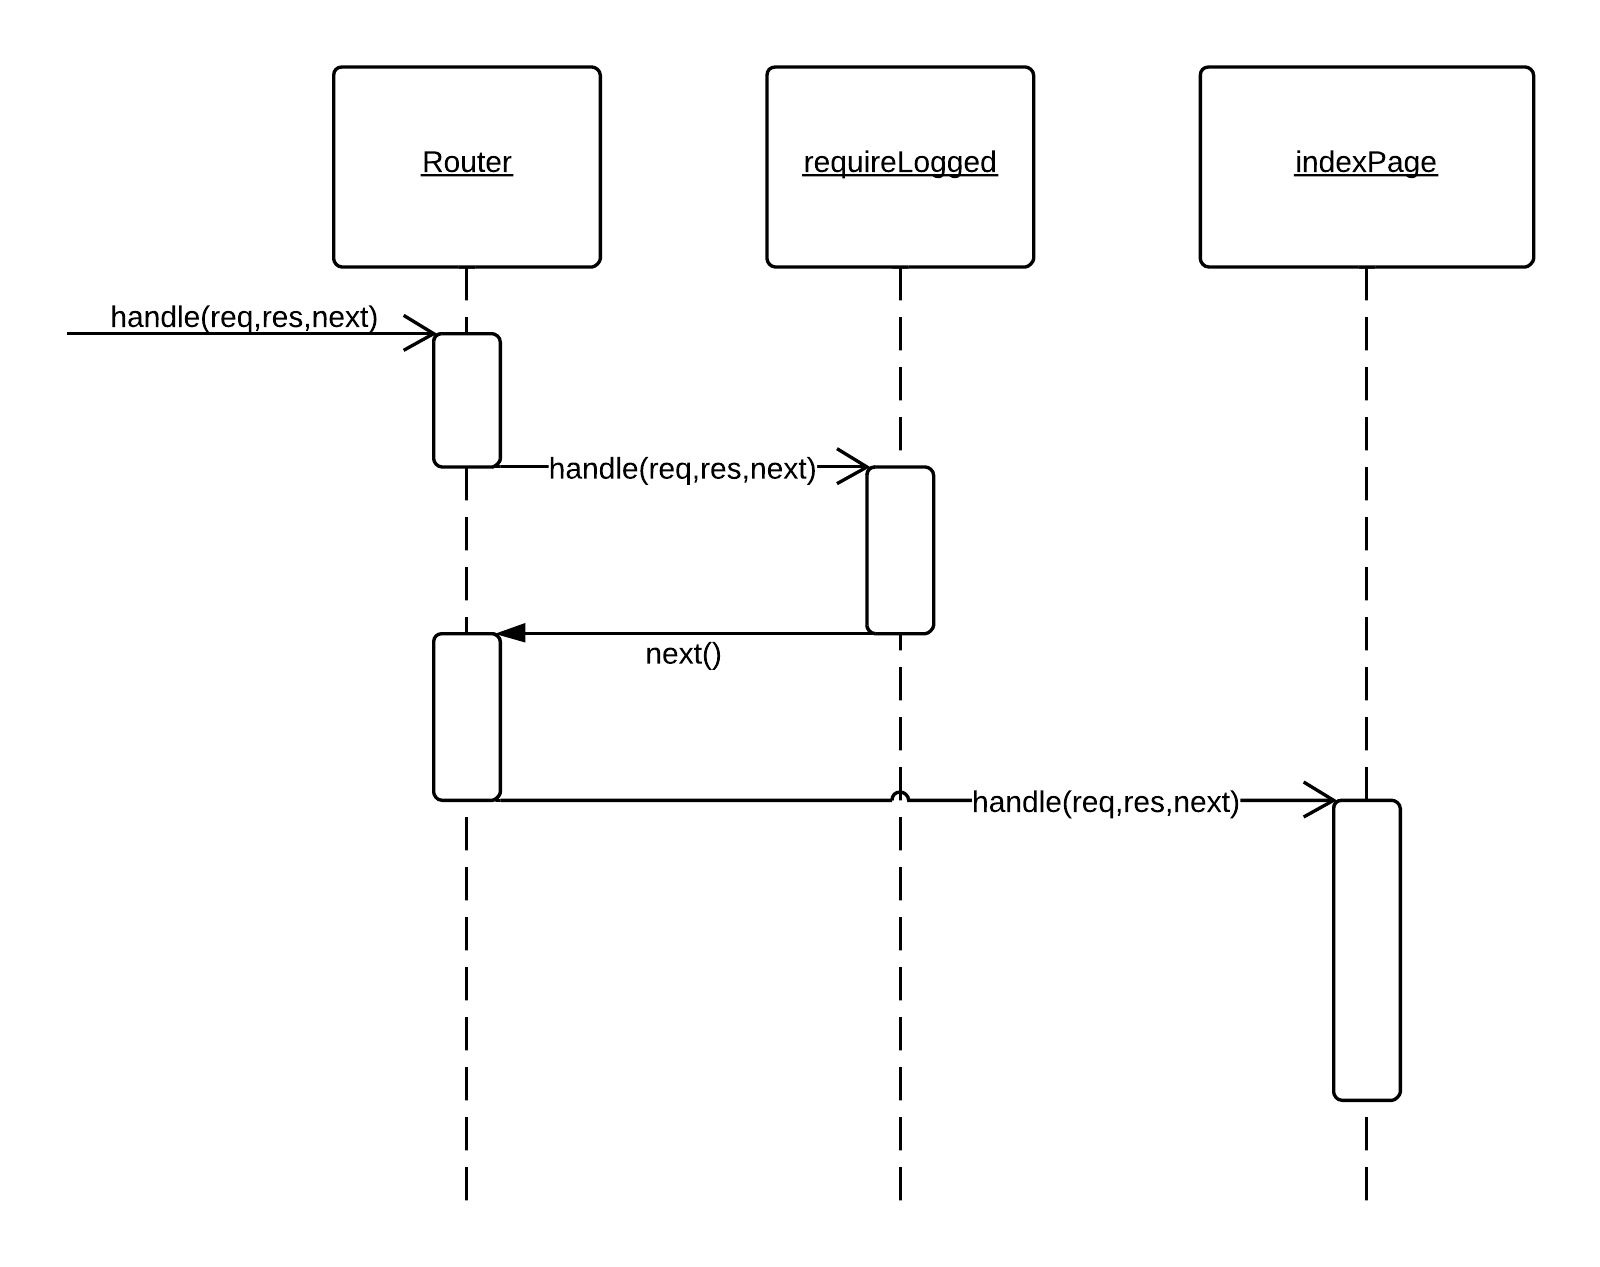
\includegraphics[scale=0.20]{scenari/Collection Name GET.png} 
		\caption{Collection Name GET}
	\end{center} 
\end{figure}

\subsubsection{Collection Name Document GET} 
Il diagramma di sequenza rappresenta lo scenario di una richiesta GET per la risorsa collection name document, nel quale al controller \emph{showpage} viene passato l'id del document di cui mostrare la show page.
\begin{figure}[H]
	\begin{center} 
		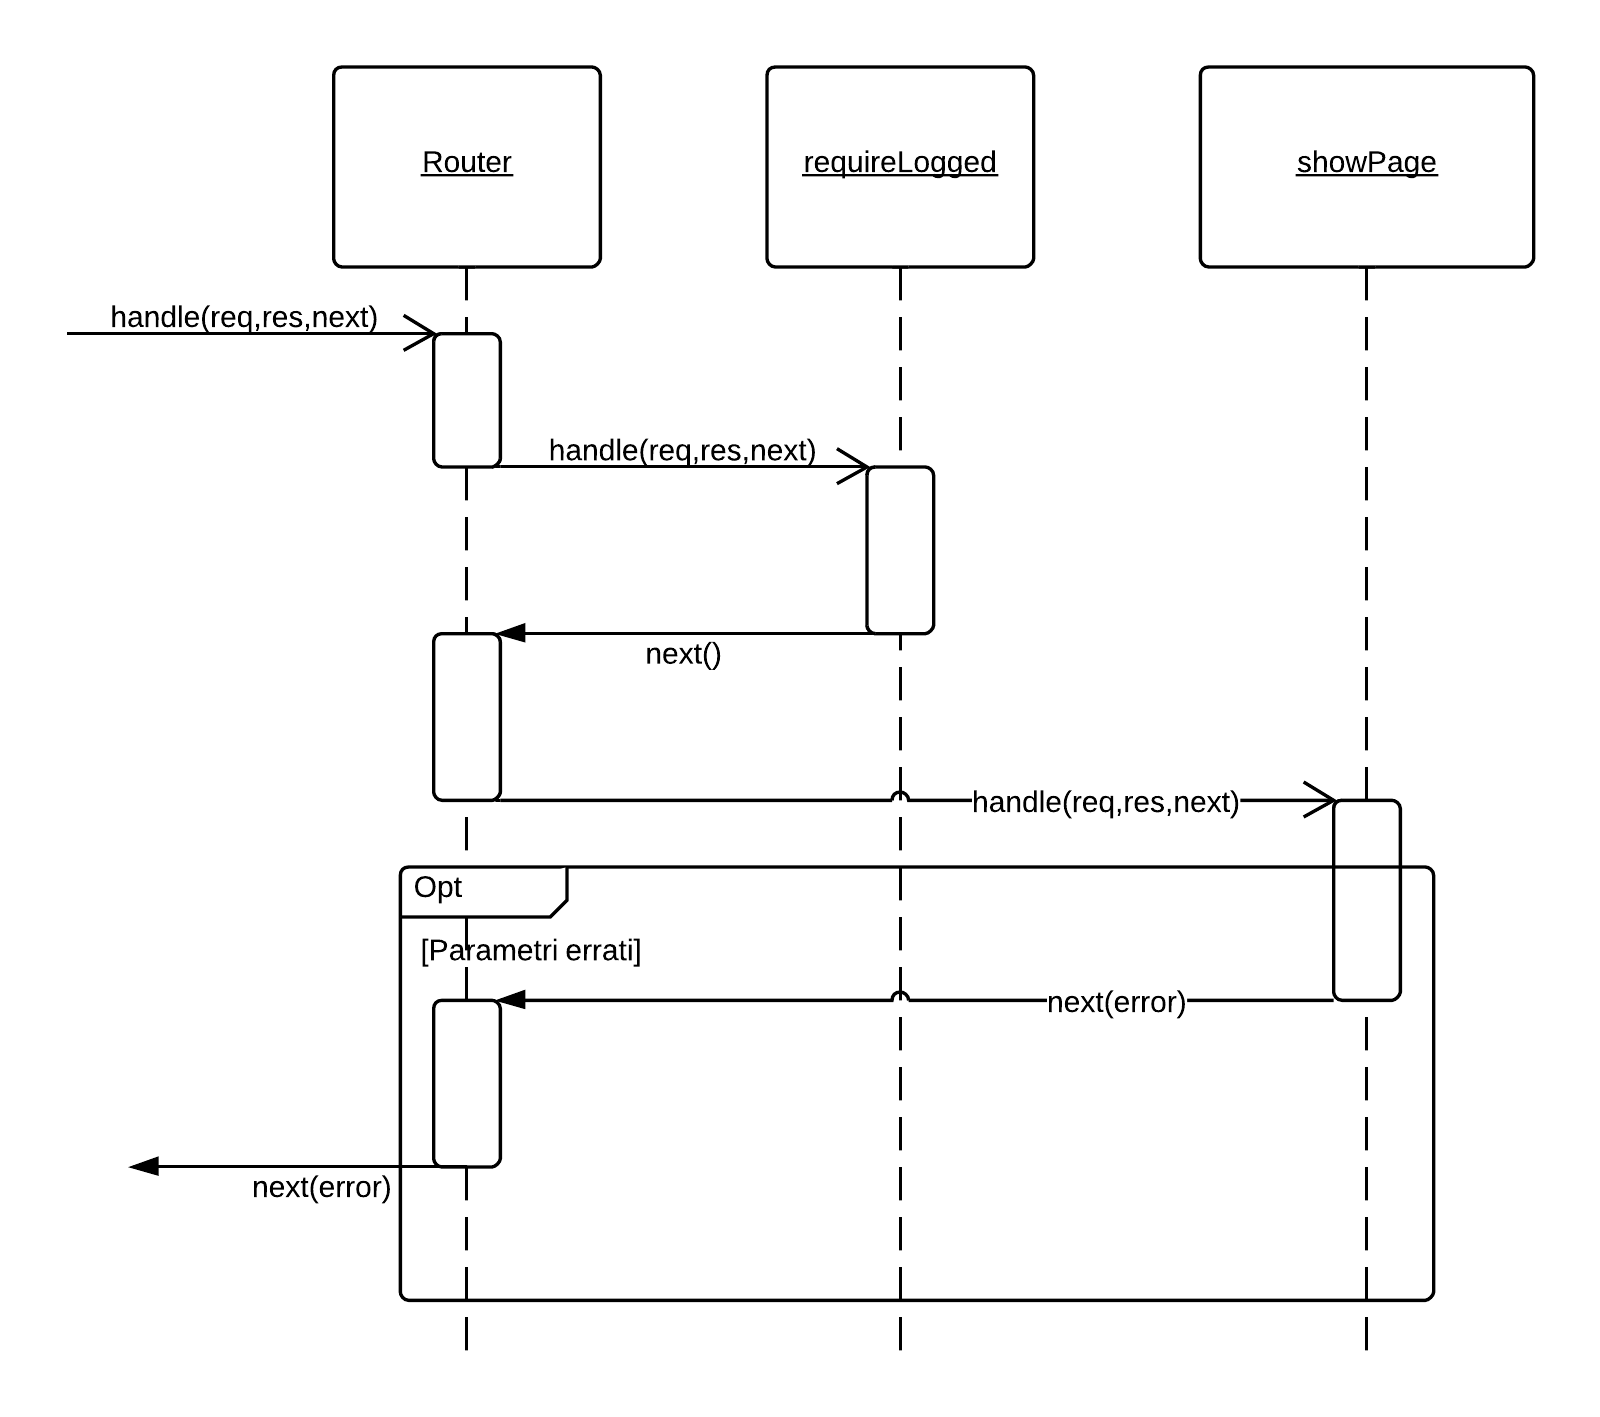
\includegraphics[scale=0.20]{scenari/Collection Name Document GET.png} 
		\caption{Collection Name Document GET}
	\end{center} 
\end{figure}

\subsubsection{Collection Name Document PUT}
Il seguente diagramma rappresenta lo scenario di una richiesta POST su una risorsa collection name document, il controller \emph{requireAdmin} non risponde con errore e viene passato il controllo a \emph{editDocument} che gestirà la richiesta.
\begin{figure}[H]
	\begin{center} 
		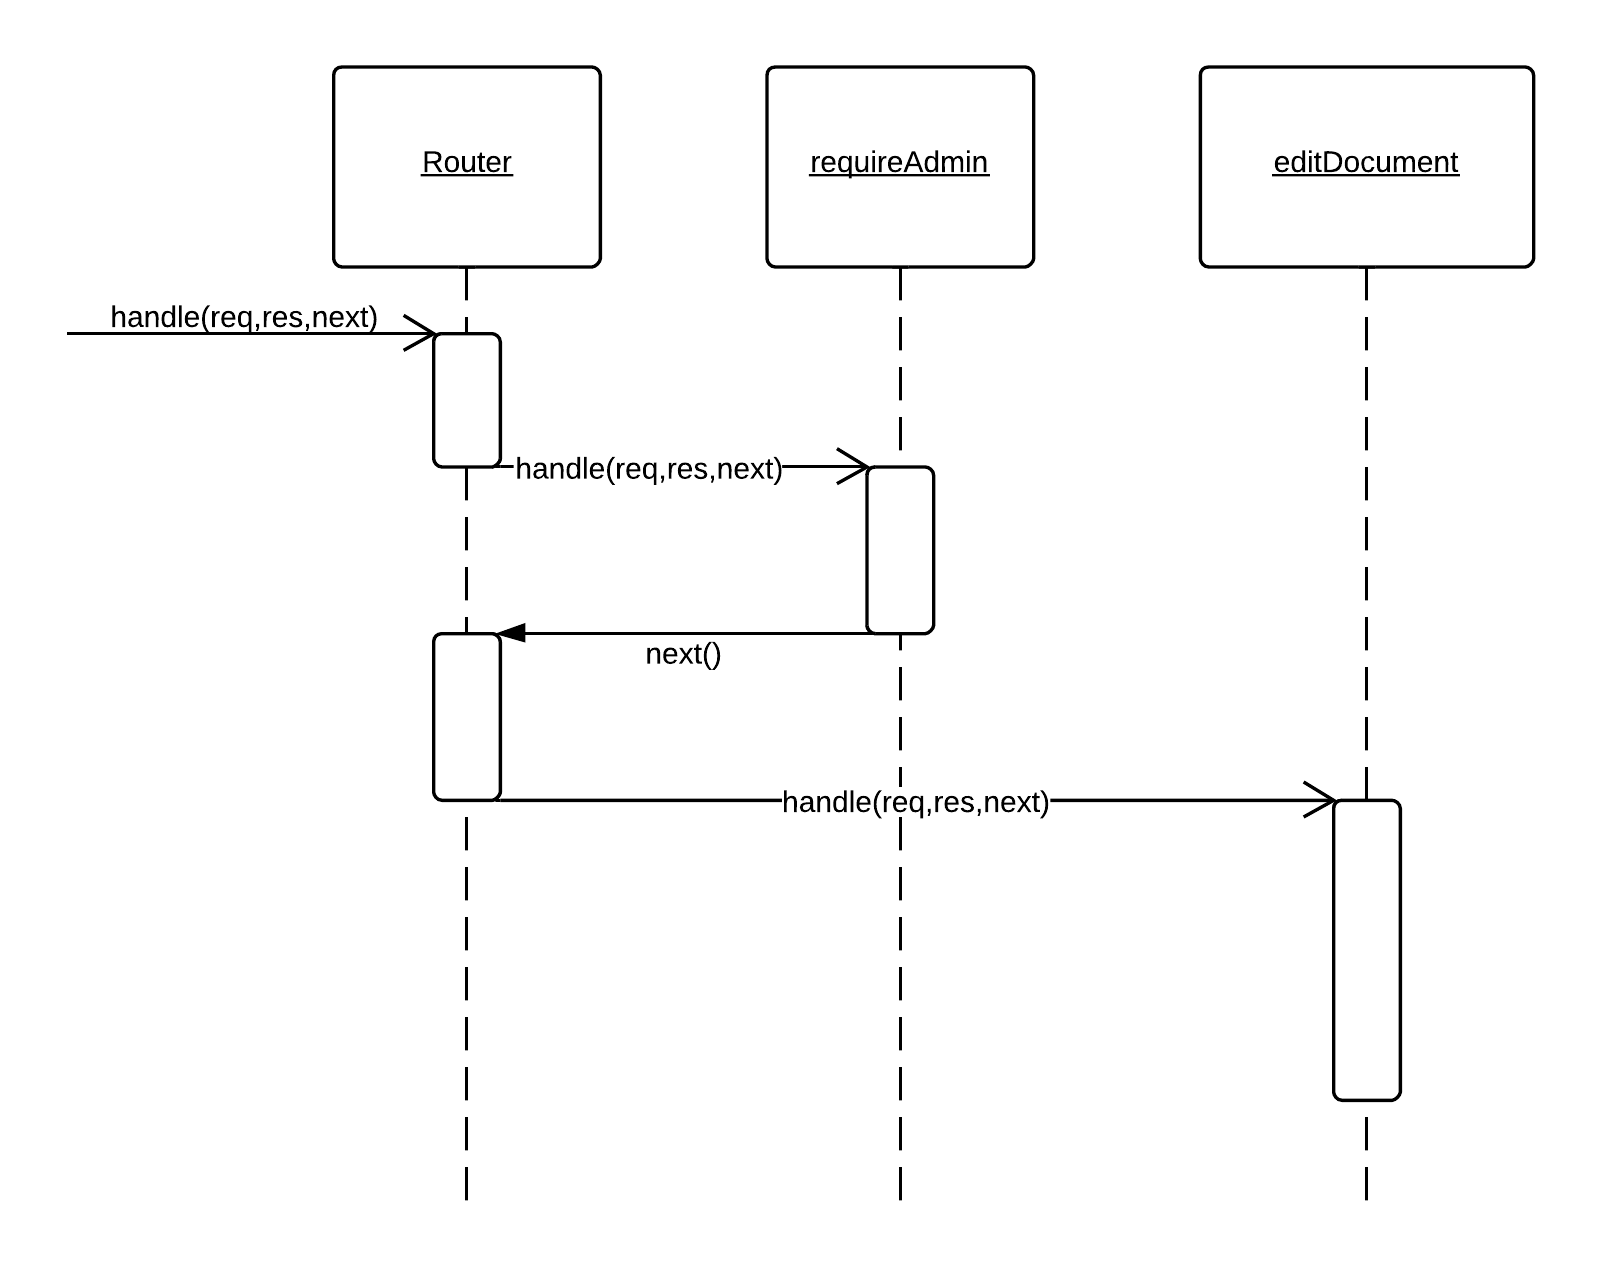
\includegraphics[scale=0.20]{scenari/Collection Name Document PUT.png} 
		\caption{Collection Name Document PUT}
	\end{center} 
\end{figure}

\subsubsection{Collection Name Document DELETE}
Il seguente scenario rappresenta la richiesta DELETE per una risorsa Collection name document, dopo che i permessi sono stati verificati il controllo è passato a \emph{deleteDocument} il quale gestirà la richiesta di eliminazione del document il cui id gli è stato passato come parametro.
\begin{figure}[H]
	\begin{center} 
		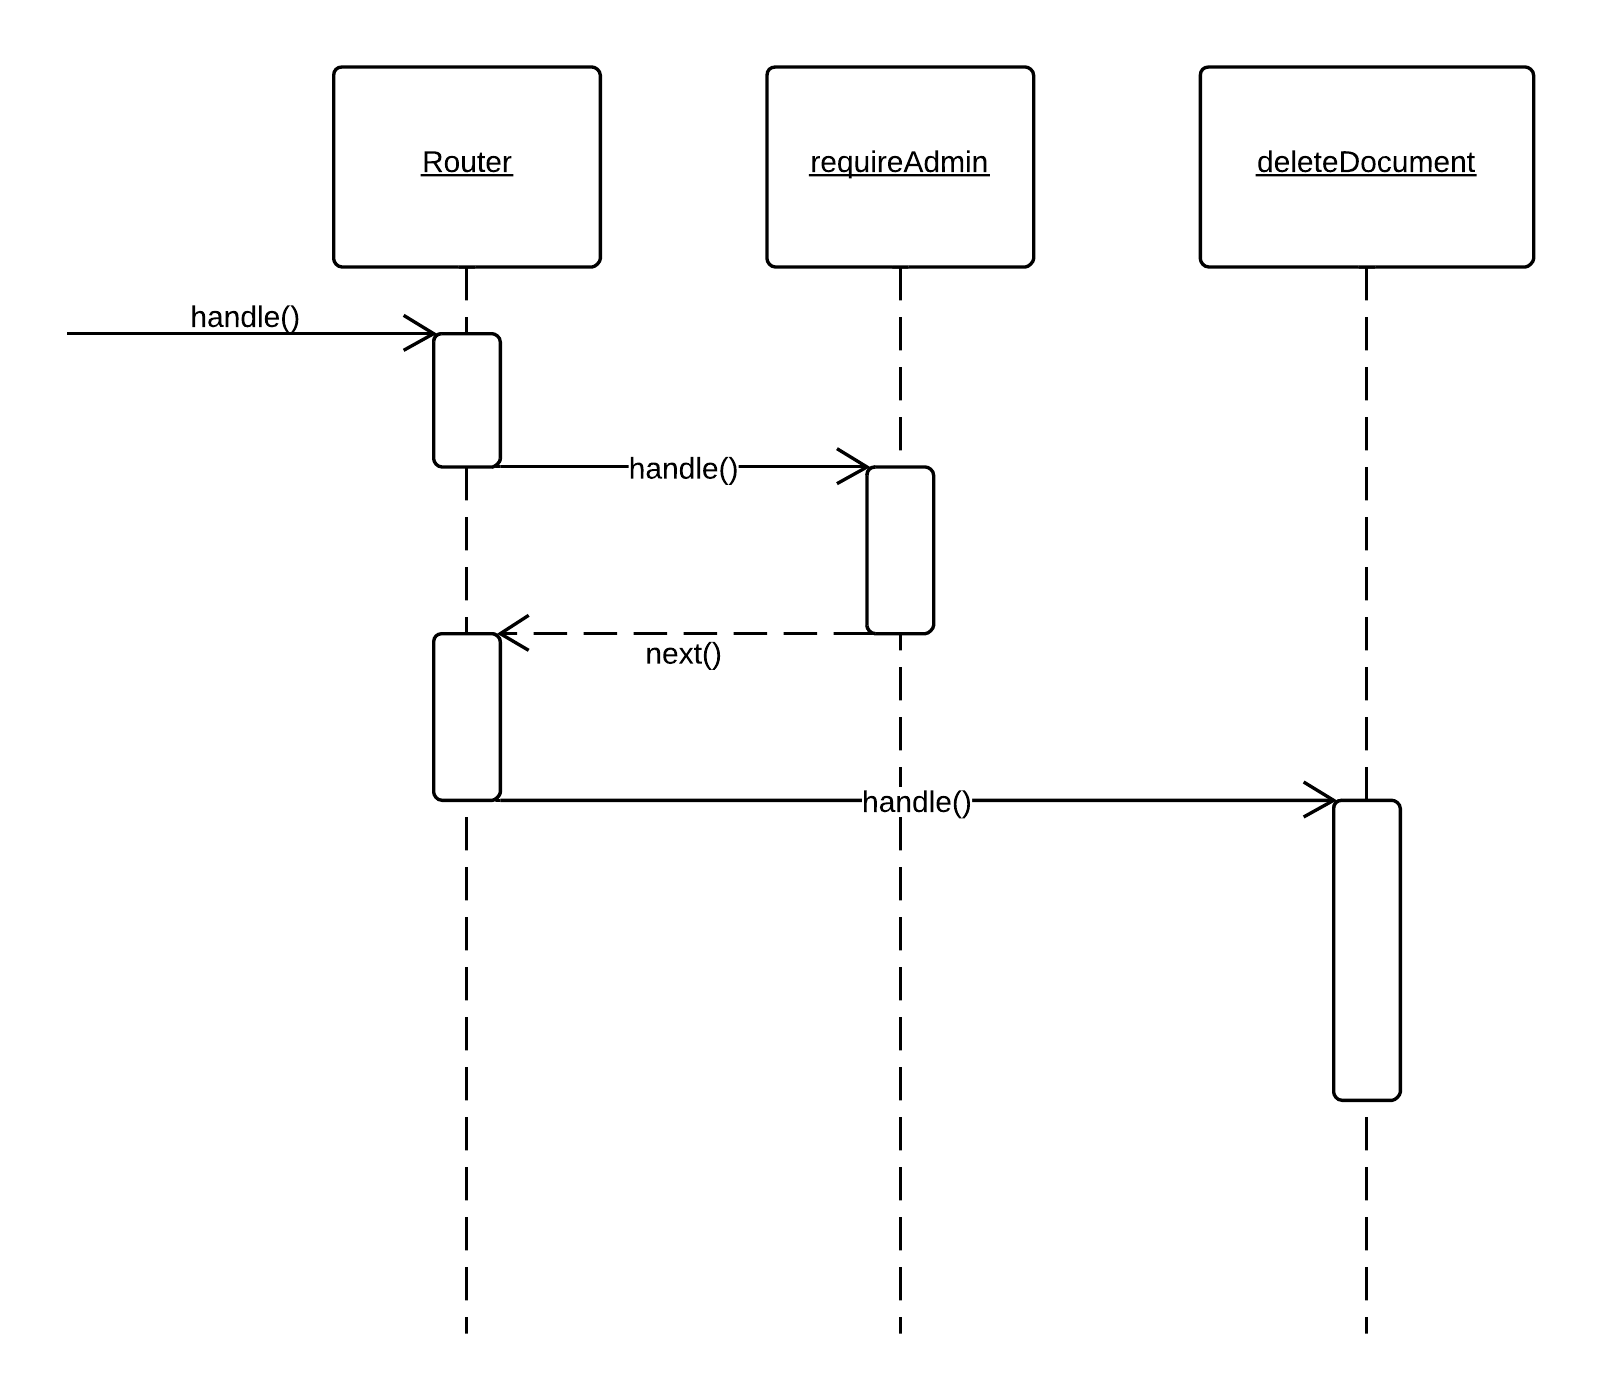
\includegraphics[scale=0.20]{scenari/Collection Name Document DELETE.png} 
		\caption{Collection Name Document DELETE}
	\end{center} 
\end{figure}

\subsubsection{Action Name Collection PUT} 
Il seguente diagramma di sequenza descrive lo scenario di una richiesta PUT per una risorsa Action name Collection.
Il controller \emph{collectionAction} si occupa di eseguire i controlli sugli attributi passatogli corrispondenti all'azione da eseguire e alla \glossario{Collection} sulla quale tale azione deve essere gestita.
\begin{figure}[H]
	\begin{center} 
		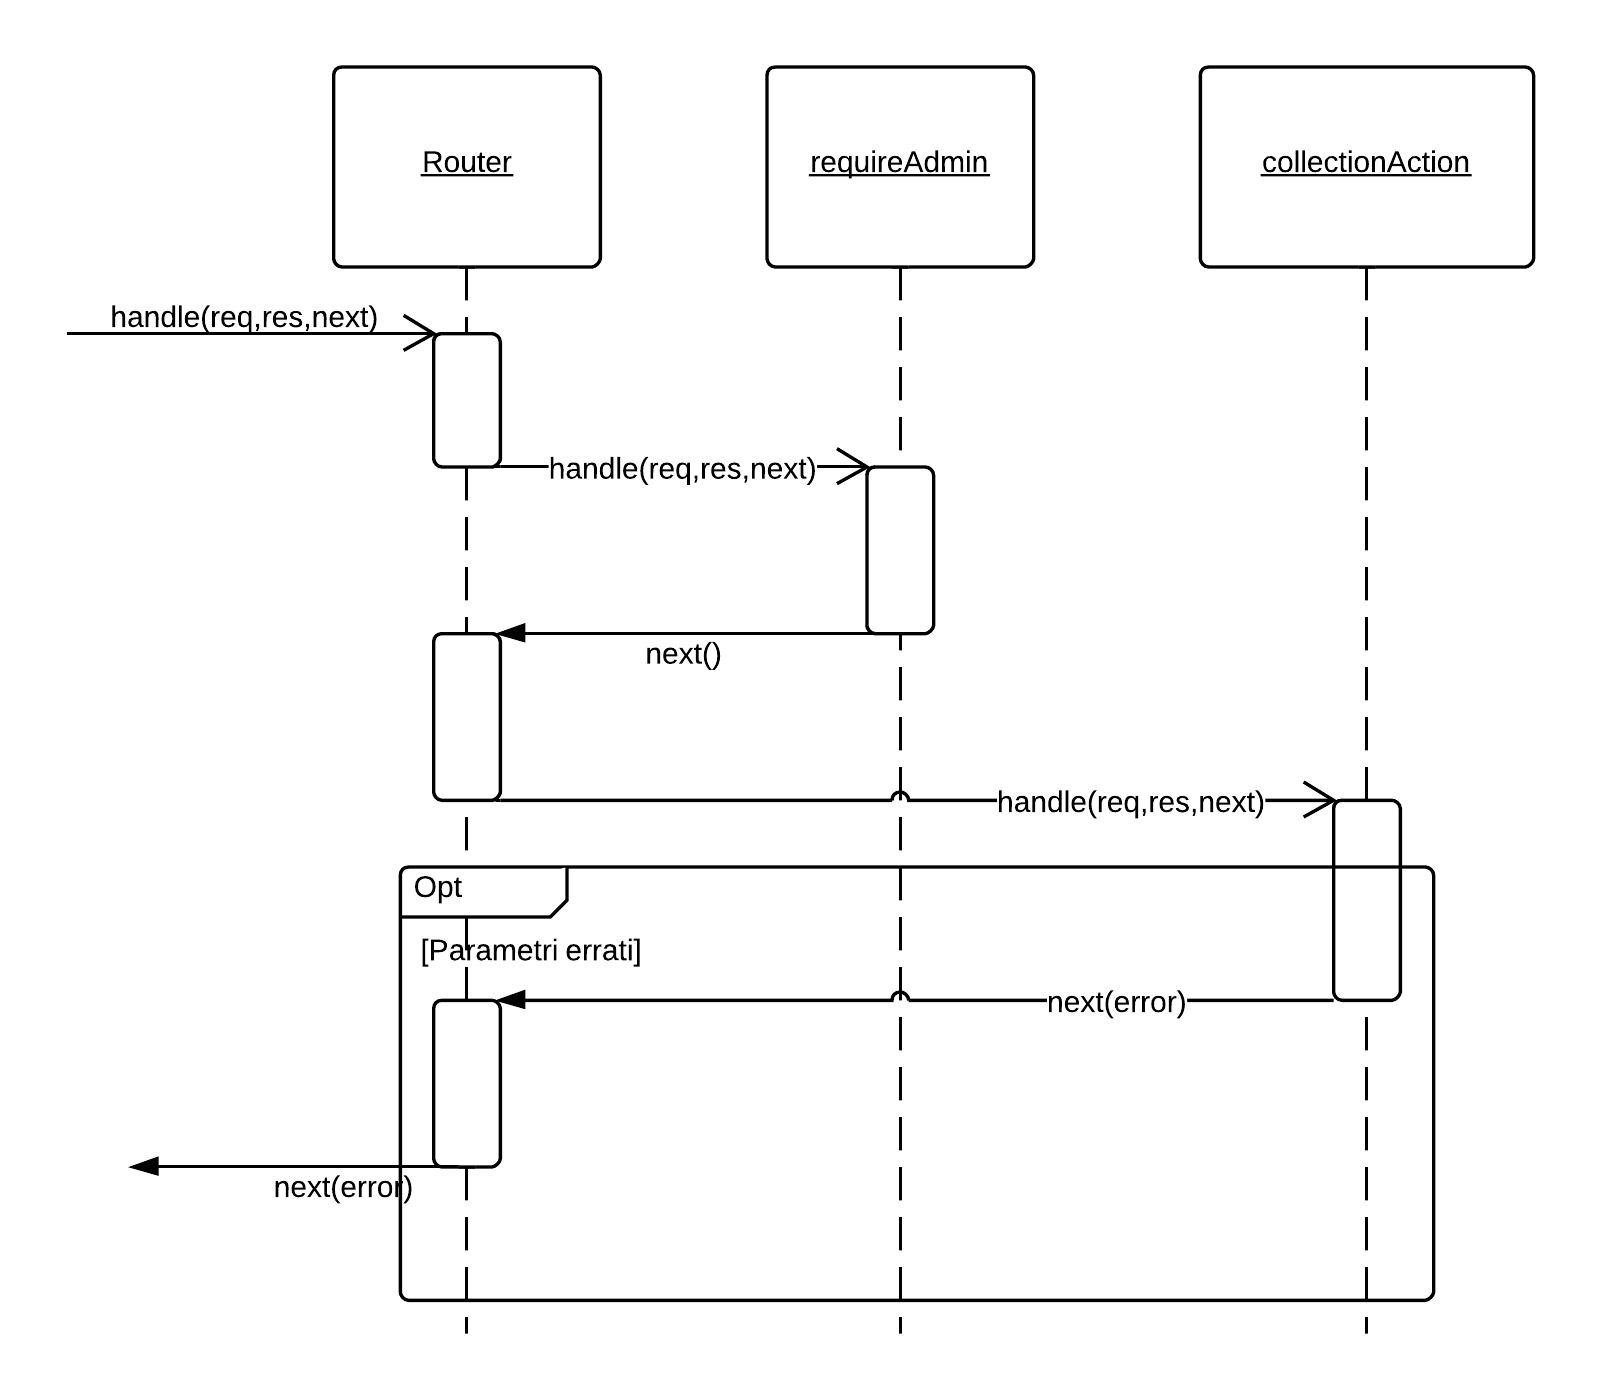
\includegraphics[scale=0.20]{scenari/Action Name Collection PUT.png} 
		\caption{Action Name Collection PUT}
	\end{center} 
\end{figure}

\subsubsection{Action Name Collection Document PUT}
Il diagramma a seguito mostrato descrive lo scenario di una richiesta PUT per la risorsa Action name Document.
Il controller \emph{documentAction} gestirà la richiesta di azione sul document corrispondente all'id passatogli come parametro.
\begin{figure}[H]
	\begin{center} 
		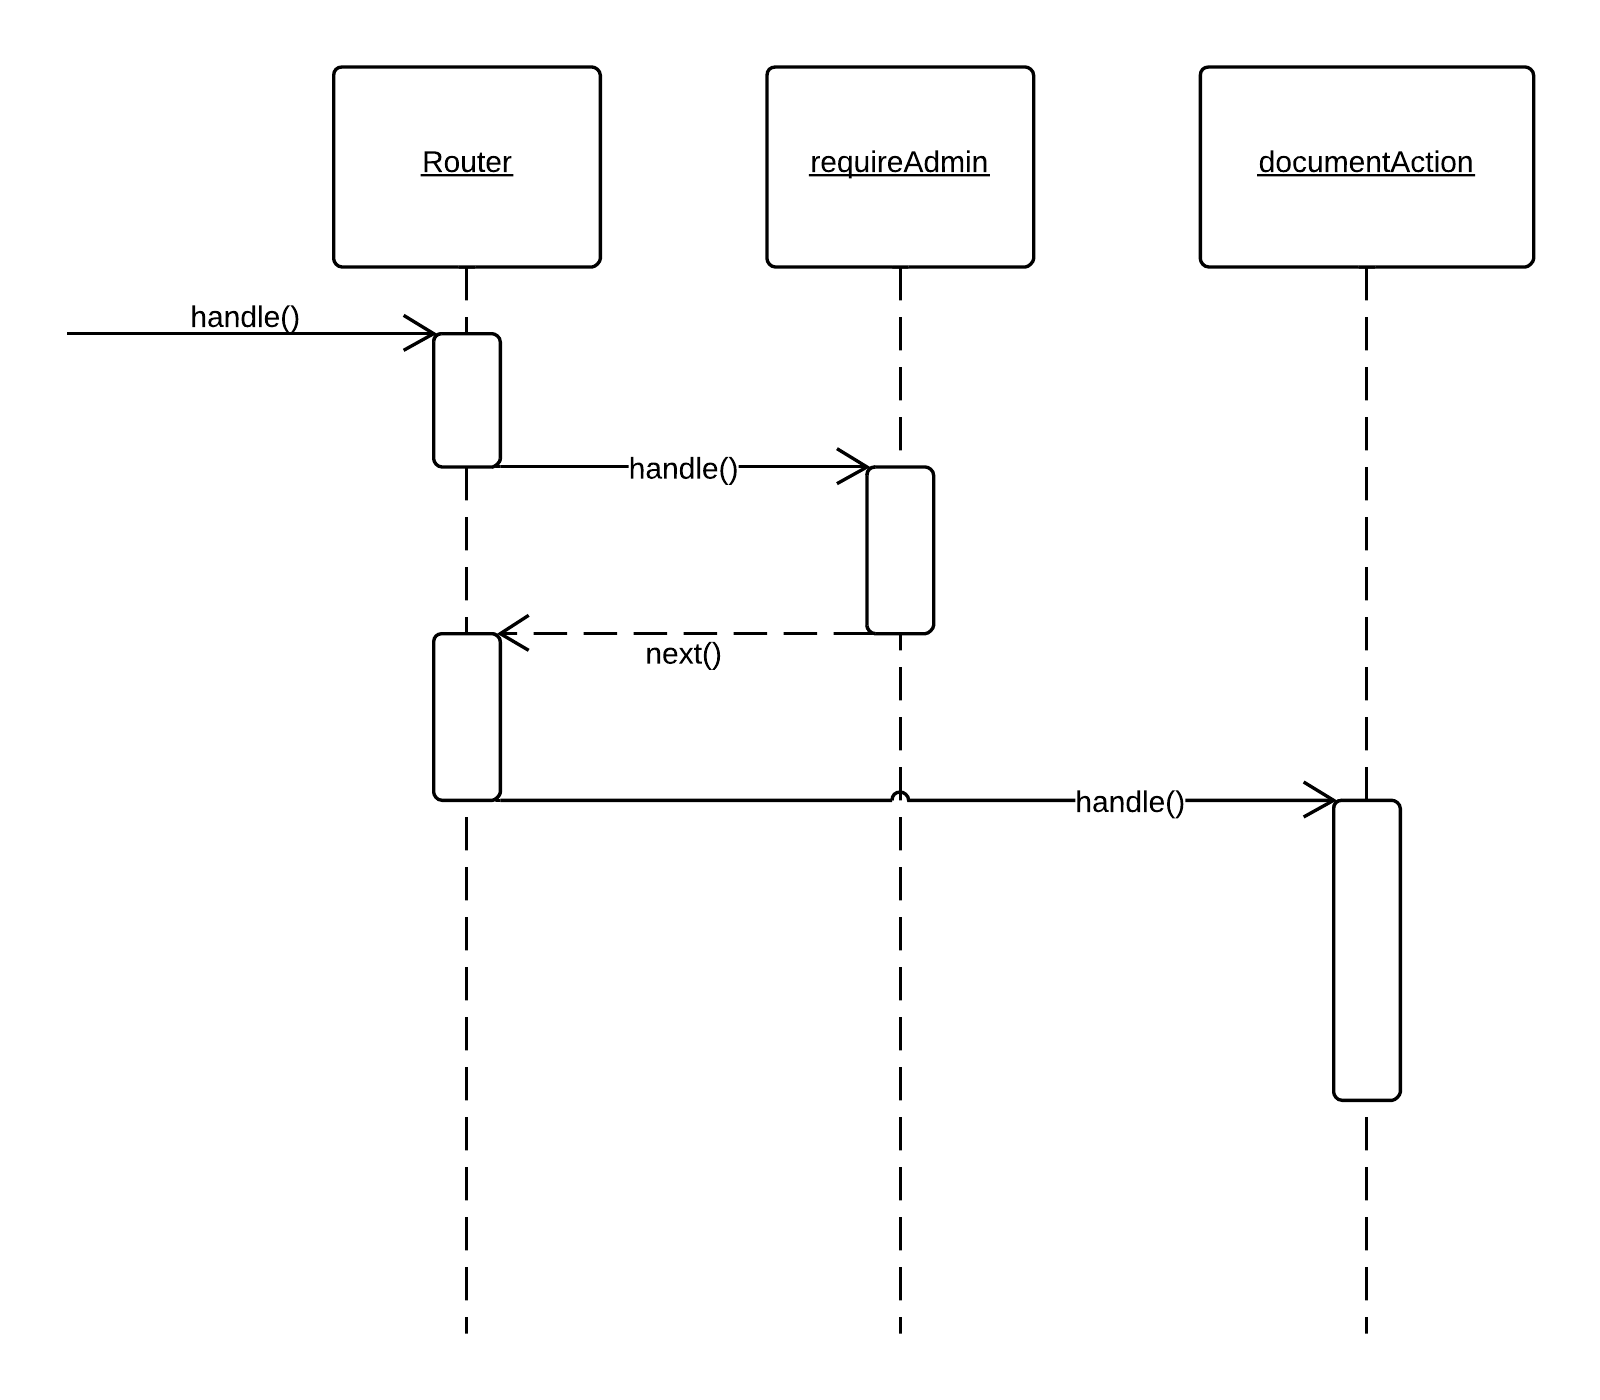
\includegraphics[scale=0.20]{scenari/Action Name Collection Document PUT.png} 
		\caption{Action Name Collection Document PUT}
	\end{center} 
\end{figure}

\subsection{Descrizione librerie aggiuntive}

Vengono di seguito descritte le librerie aggiuntive utilizzate dal Back-end. La scelta è stata effettuata cercando di valutare la diffusione, il livello di stabilità, l'assenza di errori noti.

\begin{itemize}
 \item \textbf{Passport:} è un middleware di autenticazione per \glossario{Node.js}. Estremamente flessibile e modulare, Passport può essere facilmente inserito in qualsiasi applicazione web basata su Express.
 \item \textbf{Passport-local:} è una libreria che permette di autenticare un utente con Passport usando un username e una password.
 \item \textbf{Passport-local-mongoose:} è un plugin per Mongoose che semplifica la costruzione di un sistema di autenticazione con Passport.
 \item \textbf{Nodemailer:} è un modulo che permette di mandare facilmente e-mail con Node.js, tramite \glossario{SMTP}. Supporta anche i caratteri \glossario{unicode}.
\end{itemize}

